%%%%%%%%%%%%%%%%%%%%%%%%%%%%%%%%%%%%
% Header                           %
%%%%%%%%%%%%%%%%%%%%%%%%%%%%%%%%%%%%
%
% Compilation:
%
% - Automated (Requires arara package):
%   - call: arara Peridigm_Installation_Guide.tex
% - Manual:
%   - pdflatex -> biber -> makeindex/create_glossaries.cmd -> pdflatex -> pdflatex
%   - For compilation add switch -shell-escape in your LaTeX editor:
%     pdflatex --shell-escape -synctex=1 -interaction=nonstopmode %source --extra-mem-top=60000000
%   - Compile at least 3 times for proper output
%
% In case of problems:
%
% - Increase Tex-Memory in batch with:
%   initexmf --edit-config-file pdflatex
%   add: main_memory=8000000
%   initexmf --dump=pdflatex
%
% Revisions: 2017-04-10 Martin Rädel <martin.raedel@dlr.de>
%                       Initial draft
%
% Contact:   Martin Rädel,  martin.raedel@dlr.de
%            DLR Composite Structures and Adaptive Systems
%
%                                 __/|__
%                                /_/_/_/  
%            www.dlr.de/fa/en      |/ DLR
% 
%%%%%%%%%%%%%%%%%%%%%%%%%%%%%%%%%%%%

% ---------------------------
% Build automation
% ---------------------------

% arara: pdflatex: {shell: yes, synctex: yes, interaction: nonstopmode}
% arara: pdflatex: {shell: yes, synctex: yes, interaction: nonstopmode}
% arara: biber
% arara: biber
% arara: create_glossaries
% arara: pdflatex: {shell: yes, synctex: yes, interaction: nonstopmode}
% arara: pdflatex: {shell: yes, synctex: yes, interaction: nonstopmode}
% arara: clean: { extensions: [ acn, acr, alg, aux, bbl, bcf, blg, dvi, glg, glo, gls, idx, ilg, ind, ist, lock, lof, log, lol, lot, mw, nlo, out, ps, toc, run.xml, slg, syg, syi, synctex, synctex.gz, tex.backup, user.adi ] }
% arara: clean_tex_directory
% This will work in a future release (delete the % in a%rara):
% a%rara: remove: { recursive, extensions: [ acn, acr, alg, aux, bbl, bcf, blg, dvi, glg, glo, gls, idx, ilg, ind, ist, lock, lof, log, lol, lot, mw, nlo, out, ps, toc, run.xml, slg, syg, syi, synctex, synctex.gz, tex.backup, user.adi ], directory: [ ZZZ_TikZ, ZZZ_Table ] }

% ---------------------------
% Paths
% ---------------------------

\newcommand{\peridoccommonpath}{../PeriDoX_Common}
\newcommand{\peridocliteraturepath}{../../Literature}

% ---------------------------
% Documentclass
% ---------------------------

% \RequirePackage{bootstrap}
\documentclass[%
  figures=plain,%
  listof=totoc,%                                % List of figures, tables in TOC
  bibliography=totoc,%                          % Bibliography in TOC
  fleqn,%                                       % left-align equations
]{bootstrap_dlrreprt}                           % Bootstrap of dlrreprt without Frutiger font

%%%%%%%%%%%%%%%%%%%%%%%%%%%%%%%%%%%%
% Preamble                         %
%%%%%%%%%%%%%%%%%%%%%%%%%%%%%%%%%%%%

%%%%%%%%%%%%%%%%%%%%%%%%%%%%%%%%%%%%
% Header                           %
%%%%%%%%%%%%%%%%%%%%%%%%%%%%%%%%%%%%
% 
% Preamble for the current document
% 
% Revisions: 2017-04-10 Martin R�del <martin.raedel@dlr.de>
%                       Initial draft
%               
% Contact:   Martin R�del,  martin.raedel@dlr.de
%            DLR Composite Structures and Adaptive Systems
%          
%                                 __/|__
%                                /_/_/_/  
%            www.dlr.de/fa/en      |/ DLR
% 
%%%%%%%%%%%%%%%%%%%%%%%%%%%%%%%%%%%%
% Content                          %
%%%%%%%%%%%%%%%%%%%%%%%%%%%%%%%%%%%%

% ---------------------------
% Packages
% ---------------------------

% General preamble
%%%%%%%%%%%%%%%%%%%%%%%%%%%%%%%%%%%%
% Header                           %
%%%%%%%%%%%%%%%%%%%%%%%%%%%%%%%%%%%%
% 
% Preamble
% 
% Revisions: 2017-04-10 Martin Raedel <martin.raedel@dlr.de>
%                       Initial draft
%               
% Contact:   Martin Raedel,  martin.raedel@dlr.de
%            DLR Composite Structures and Adaptive Systems
%          
%                                 __/|__
%                                /_/_/_/  
%            www.dlr.de/fa/en      |/ DLR
% 
%%%%%%%%%%%%%%%%%%%%%%%%%%%%%%%%%%%%
% Content                          %
%%%%%%%%%%%%%%%%%%%%%%%%%%%%%%%%%%%%

%%%%%%%%%%%%%%%%%%%%%%%%%%%%%%%%%%%%
% Header                           %
%%%%%%%%%%%%%%%%%%%%%%%%%%%%%%%%%%%%
% 
% This file handles all things with general packages
% 
% Revisions: 2017-04-10 Martin Raedel <martin.raedel@dlr.de>
%                       Initial draft
%               
% Contact:   Martin Raedel,  martin.raedel@dlr.de
%            DLR Composite Structures and Adaptive Systems
%          
%                                 __/|__
%                                /_/_/_/  
%            www.dlr.de/fa/en      |/ DLR
% 
%%%%%%%%%%%%%%%%%%%%%%%%%%%%%%%%%%%%
% Content                          %
%%%%%%%%%%%%%%%%%%%%%%%%%%%%%%%%%%%%

% ---------------------------
% Packages
% ---------------------------

% Every package with the exception of
% - RMLaTeX-packages
% - Hyperref
% - Every package that has to be placed after hyperref -> Pref_Packages_Hyperref.tex
\usepackage[latin1]{inputenx}
\usepackage[T1]{fontenc}
\usepackage{amsmath}
\usepackage{amssymb}
\usepackage{amsthm}
\usepackage[page,titletoc]{appendix}
\usepackage{array}
% babel package is loaded seperately. Allows reuse for projects with various languages
% biblatex package is loaded in Pref_BibLaTeX_XYZ.tex from PeriDoc_Common
\usepackage{booktabs}
\usepackage{caption}
\usepackage{calc}
\usepackage{color}
\usepackage{coseoul}
\usepackage{csquotes}
\usepackage{enumitem}
\usepackage{esvect}
\usepackage{etoolbox}
\usepackage{filecontents}
% http://tex.stackexchange.com/a/312910/44634 for fixing clash between filecontents and morewrites
\newwrite\fcwrite
\makeatletter
\let\zzzz\filec@ntents
\def\filec@ntents{\def\chardef##1\write{\let\reserved@c\fcwrite}\zzzz}
\makeatother
% Mute "Overwriting file" warning for filecontents package
\usepackage{ifthen}
\usepackage{ltxtable}
\usepackage{marginnote}
\usepackage{marvosym}                            % Symbols: \Faxmachine, \Mundus, \Letter
\usepackage{mathtools}
\usepackage{mdframed}
\usepackage{media9}
\usepackage{morewrites}                          % http://tex.stackexchange.com/q/289734
\usepackage{multicol}
\usepackage{multirow}
%\usepackage{nomencl}
\usepackage{pifont}
\usepackage{placeins}
\usepackage{subcaption}
\usepackage{tabto}
\usepackage{tabu}
\usepackage{tabularx}
\usepackage[most]{tcolorbox}
\usepackage{textcomp}

\makeatletter
\@ifundefined{KOMAClassName}
  {% true -> no KOMA class
    \@ifclassloaded{amsart}{
      % Do nothing! Amsart does not play with titlesec package
    }{
      \usepackage{titlesec}    
    }
  }
  {% false -> KOMA class
  }
\makeatother

\usepackage[figure,table,lstlisting]{totalcount}
\usepackage{upquote}
\usepackage{wasysym}                            % Symbols \& Smileys :)
\usepackage{wrapfig}
\usepackage{xparse}

\usepackage{hyphenat}

\makeatletter%
  \@ifclassloaded{dlrreprt}{%%%%%%%%%%%%%%%%%%%%%%%%%%%%%%%%%%%%
% Header                           %
%%%%%%%%%%%%%%%%%%%%%%%%%%%%%%%%%%%%
% 
% This file handles all things considering DLR packages
% 
% Revisions: 2017-04-10 Martin Raedel <martin.raedel@dlr.de>
%                       Initial draft
%               
% Contact:   Martin Raedel,  martin.raedel@dlr.de
%            DLR Composite Structures and Adaptive Systems
%          
%                                 __/|__
%                                /_/_/_/  
%            www.dlr.de/fa/en      |/ DLR
% 
%%%%%%%%%%%%%%%%%%%%%%%%%%%%%%%%%%%%
% Content                          %
%%%%%%%%%%%%%%%%%%%%%%%%%%%%%%%%%%%%

\usepackage{dlrsecondpage}
\usepackage{listofversions}}{}
  \@ifclassloaded{dlrbook}{%%%%%%%%%%%%%%%%%%%%%%%%%%%%%%%%%%%%
% Header                           %
%%%%%%%%%%%%%%%%%%%%%%%%%%%%%%%%%%%%
% 
% This file handles all things considering DLR packages
% 
% Revisions: 2017-04-10 Martin Raedel <martin.raedel@dlr.de>
%                       Initial draft
%               
% Contact:   Martin Raedel,  martin.raedel@dlr.de
%            DLR Composite Structures and Adaptive Systems
%          
%                                 __/|__
%                                /_/_/_/  
%            www.dlr.de/fa/en      |/ DLR
% 
%%%%%%%%%%%%%%%%%%%%%%%%%%%%%%%%%%%%
% Content                          %
%%%%%%%%%%%%%%%%%%%%%%%%%%%%%%%%%%%%

\usepackage{dlrsecondpage}
\usepackage{listofversions}}{}
\makeatother%

%%%%%%%%%%%%%%%%%%%%%%%%%%%%%%%%%%%%
% Header                           %
%%%%%%%%%%%%%%%%%%%%%%%%%%%%%%%%%%%%
% 
% Preference file for everything considering glossaries
% 
% Revisions: 2017-04-10 Martin Raedel <martin.raedel@dlr.de>
%                       Initial draft
%               
% Contact:   Martin Raedel,  martin.raedel@dlr.de
%            DLR Composite Structures and Adaptive Systems
%          
%                                 __/|__
%                                /_/_/_/  
%            www.dlr.de/fa/en      |/ DLR
% 
%%%%%%%%%%%%%%%%%%%%%%%%%%%%%%%%%%%%
% Content                          %
%%%%%%%%%%%%%%%%%%%%%%%%%%%%%%%%%%%%

%%%%%%%%%%%%%%%%%%%%%%%%%%%%%%%%%%%%
% Package                          %
%%%%%%%%%%%%%%%%%%%%%%%%%%%%%%%%%%%%

\usepackage[
%   nonumberlist,   %keine Seitenzahlen anzeigen
  acronym,        %ein Abk�rzungsverzeichnis erstellen
  nomain,         %don�t use the main glossary
  toc,            %Eintr�ge im Inhaltsverzeichnis
  %translate=babel,
  %section=\glossarytoclevel   % kapitelweise Verzeichniserstellung
%   section,        %im Inhaltsverzeichnis auf section-Ebene erscheinen
%   savewrites,     % minimise the number of write registers used
]{glossaries}

% \usepackage{scrwfile} % No \newwrite and therefore limitations on registers

%%%%%%%%%%%%%%%%%%%%%%%%%%%%%%%%%%%%
% Redefine package options         %
%%%%%%%%%%%%%%%%%%%%%%%%%%%%%%%%%%%%

%Den Punkt am Ende jeder Beschreibung deaktivieren
\renewcommand*{\glspostdescription}{}
% \renewcommand*{\glspostdescription}{\dotfill}

%%%%%%%%%%%%%%%%%%%%%%%%%%%%%%%%%%%%
% Own styles                       %
%%%%%%%%%%%%%%%%%%%%%%%%%%%%%%%%%%%%

% -----------------
% Acronym-styles
% -----------------

\newglossarystyle{myacronymstyle}{%
  \renewenvironment{theglossary}%
    {\begin{longtabu} to \linewidth {lX}}%
    {\end{longtabu}}%
  % Header line
  \renewcommand*{\glossaryheader}{%
%     % Requires booktabs
%     \toprule%
%     Abbreviation & Description%
%     \tabularnewline%
%     \midrule%
%     \endhead%
%     \bottomrule%
%     \endfoot%
  }%
  % indicate what to do at the start of each logical group
  %\renewcommand*{\glsgroupheading}[1]{}%
  %\renewcommand*{\glsgroupskip}{}% What to do between groups
  \renewcommand*{\glsgroupskip}{\tabularnewline}% What to do between groups
  \renewcommand*{\glossaryentryfield}[5]{%
    \glsentryitem{##1}\glstarget{##1}{##2} 
     %\glstarget{##2}{##2}% Name
      & ##3\glspostdescription ##5% Description
      \\% end of row
  }
}


    \newglossarystyle{myglostyle}{%
      \renewcommand*{\glsclearpage}{}%
      \renewenvironment{theglossary}%
        {\begin{longtabu} to \linewidth {cX}}%
        {\end{longtabu}}%
      % Header line
      \renewcommand*{\glossaryheader}{%
        \textbf{Symbol} & \textbf{Description}%
        \tabularnewline%
        \tabularnewline%
        \endhead%
        \endfoot%
      }%
      \renewcommand*{\glsgroupskip}{\tabularnewline}
      \renewcommand*{\glossentry}[1]{%
        \glsentryitem{##1}
        \glstarget{##1}{\glossentrysymbol{##1}} &
        \glossentrydesc{##1}        %& % Description
        \tabularnewline%
      }%
    }

% -----------------
% Coordinate-system style
% -----------------

\newglossarystyle{mycoordinatesystemstyle}{%
  %\renewcommand{\glossarysection}[2][]{}% no title
  \renewcommand*{\glsclearpage}{}% avoid page break before glossary
  \renewenvironment{theglossary}%
    % \extrarowsep=1mm
    {\begin{longtabu} to \linewidth {cX}}%
    {\end{longtabu}}%
  % Header line
  \renewcommand*{\glossaryheader}{%
    % Requires booktabs
    %\toprule%
    \textbf{Symbol} & \textbf{Description}%
    \tabularnewline%
    \tabularnewline%
    %\midrule%
    \endhead%
    %\bottomrule%
    \endfoot%
  }%
  % indicate what to do at the start of each logical group
  %\renewcommand*{\glsgroupheading}[1]{}%
  %\renewcommand*{\glsgroupskip}{}% What to do between groups
  \renewcommand*{\glsgroupskip}{\tabularnewline}% What to do between groups
%   \renewcommand*{\glossaryentryfield}[5]{%
%     \glsentryitem{##1}\glstarget{##1}{##2} 
%      %\glstarget{##2}{##2}% Name
%       & ##3\glspostdescription ##5% Description
%       \\% end of row
%   }
  \renewcommand*{\glossentry}[1]{%
    \glsentryitem{##1}% Entry number if required
    \glstarget{##1}{\glossentrysymbol{##1}} &
    %\glossentrysymbol{##1}	& % Symbol
    %\glossentryname{##1}	& % Name
    \glossentrydesc{##1}	%& % Description
    %\glsentryuseri{##1}%	  % Unit in User1-Variable
    \tabularnewline%
  }%
}

% -----------------
% Symbols-styles
% -----------------

\newglossarystyle{mysymbolstyle}{%
  %\renewcommand{\glossarysection}[2][]{}% no title
  \renewcommand*{\glsclearpage}{}% avoid page break before glossary
  \renewenvironment{theglossary}%
    % \extrarowsep=1mm
    {\begin{longtabu} to \linewidth {clX}}%c}}%
    {\end{longtabu}}%
%     {\begin{longtable}{@{}p{0.1\linewidth}p{0.8\linewidth}p{0.1\linewidth}@{}}}%
%     {\end{longtable}}%
  % Header line
  \renewcommand*{\glossaryheader}{%
    % Requires booktabs
    %\toprule%
    \textbf{Symbol} & \textbf{Name} & \textbf{Description}% & \textbf{Unit}%
    \tabularnewline%
    \tabularnewline%
    %\midrule%
    \endhead%
    %\bottomrule%
    \endfoot%
  }%
  % indicate what to do at the start of each logical group
  %\renewcommand*{\glsgroupheading}[1]{}%
  %\renewcommand*{\glsgroupskip}{}% What to do between groups
  \renewcommand*{\glsgroupskip}{\tabularnewline}% What to do between groups
%   \renewcommand*{\glossaryentryfield}[5]{%
%     \glsentryitem{##1}\glstarget{##1}{##2} 
%      %\glstarget{##2}{##2}% Name
%       & ##3\glspostdescription ##5% Description
%       \\% end of row
%   }
  \renewcommand*{\glossentry}[1]{%
    \glsentryitem{##1}% Entry number if required
    \glstarget{##1}{\glossentrysymbol{##1}} &
    %\glossentrysymbol{##1}	& % Symbol
    \glossentryname{##1}	& % Name
    \glossentrydesc{##1}	%& % Description
    %\glsentryuseri{##1}%	  % Unit in User1-Variable
    \tabularnewline%
  }%
}

% -----------------
% Symbols-styles for papers
% -----------------

\newglossarystyle{myonecolpapersymbolstyle}{%
  %\renewcommand{\glossarysection}[2][]{}% no title
  \renewcommand*{\glsclearpage}{}% avoid page break before glossary
  \renewenvironment{theglossary}%
    {\begin{longtabu} to \linewidth {clXcl}}%c}}%
    {\end{longtabu}}%
  % Header line
  \renewcommand*{\glossaryheader}{}%
  %\renewcommand*{\glsgroupheading}[1]{}% indicate what to do at the start of each logical group
  \renewcommand*{\glsgroupskip}{}% What to do between groups -> no skip
  \renewcommand*{\glossentry}[1]{% How the entry looks like
    \glsentryitem{##1}% Entry number if required
    \glstarget{##1}{\glossentrysymbol{##1}} & % Symbol
    \glossentryname{##1}        %& % Name
    \tabularnewline%
  }%
}

% https://tex.stackexchange.com/a/216434/44634
% needs: \usepackage{multicol}
\newglossarystyle{mytwocolpapersymbolstyle}{%
  %\renewcommand{\glossarysection}[2][]{}% no title
  \renewenvironment{theglossary}%
    {\begin{multicols}{2}\raggedright}
    {\end{multicols}}
  % Header line
  \renewcommand*{\glossaryheader}{}%
  \renewcommand*{\glsgroupheading}[1]{}% indicate what to do at the start of each logical group
  \renewcommand*{\glsgroupskip}{}% What to do between groups -> no skip
  \renewcommand*{\glsclearpage}{}% avoid page break before glossary 
  % set how each entry should appear:
  \renewcommand*{\glossentry}[2]{
    \noindent\makebox[2.5em][c]{\glstarget{##1}{\glossentrysymbol{##1}}}% Symbol
    \glossentryname{##1}% Name
    \newline
  }
%   \renewcommand*{\subglossentry}[3]{%
%     \glossentry{##2}{##3}
%   }
}

% -----------------
% Exponent-styles
% -----------------

\newglossarystyle{myexponentstyle}{%
  %\renewcommand{\glossarysection}[2][]{}% no title
  \renewcommand*{\glsclearpage}{}% avoid page break before glossary
  \renewenvironment{theglossary}%
    % \extrarowsep=1mm
    {%
      \begingroup
      \renewcommand{\arraystretch}{1.4}
      \begin{longtabu} to \linewidth {@{\ \ }r@{}lX}
    }{%
      \end{longtabu}
      \endgroup
    }%
%     {\begin{longtable}{@{}p{0.1\linewidth}p{0.8\linewidth}p{0.1\linewidth}@{}}}%
%     {\end{longtable}}%
  % Header line
  \renewcommand*{\glossaryheader}{%
    % Requires booktabs
    %\toprule%
    %\textbf{Symbol} & \textbf{Name} & \textbf{Description}%
    \multicolumn{2}{@{}c@{}}{\textbf{Symbol}} & \textbf{Description}%
    \tabularnewline%
    \tabularnewline%
    %\midrule%
    \endhead%
    %\bottomrule%
    \endfoot%
  }%
  % indicate what to do at the start of each logical group
  %\renewcommand*{\glsgroupheading}[1]{}%
  %\renewcommand*{\glsgroupskip}{}% What to do between groups
  \renewcommand*{\glsgroupskip}{\tabularnewline}% What to do between groups
%   \renewcommand*{\glossaryentryfield}[5]{%
%     \glsentryitem{##1}\glstarget{##1}{##2} 
%      %\glstarget{##2}{##2}% Name
%       & ##3\glspostdescription ##5% Description
%       \\% end of row
%   }
  \renewcommand*{\glossentry}[1]{%
    \glsentryitem{##1}% Entry number if required
    \protect\ensuremath{\protect\left(\protect\phantom{a}\protect\right)} &
    \glstarget{##1}{\protect\ensuremath{\protect\vphantom{a}^{\glossentrysymbol{##1}}}} &
    %\glossentrysymbol{##1}     & % Symbol
    %\glossentryname{##1}       & % Name
    \glossentrydesc{##1}        %& % Description
    %\glsentryuseri{##1}%         % Unit in User1-Variable
    \tabularnewline%
  }%
}

% -----------------
% Index-styles
% -----------------

\newglossarystyle{myindexstyle}{%
  %\renewcommand{\glossarysection}[2][]{}% no title
  \renewcommand*{\glsclearpage}{}% avoid page break before glossary
  \renewenvironment{theglossary}%
    % \extrarowsep=1mm
    {%
      \begingroup
      \renewcommand{\arraystretch}{1.4}
      \begin{longtabu} to \linewidth {@{\ \ }r@{}lX}
    }{%
      \end{longtabu}
      \endgroup
    }%
%     {\begin{longtable}{@{}p{0.1\linewidth}p{0.8\linewidth}p{0.1\linewidth}@{}}}%
%     {\end{longtable}}%
  % Header line
  \renewcommand*{\glossaryheader}{%
    % Requires booktabs
    %\toprule%
    %\textbf{Symbol} & \textbf{Name} & \textbf{Description}%
    \multicolumn{2}{@{}c@{}}{\textbf{Symbol}} & \textbf{Description}%
    \tabularnewline%
    \tabularnewline%
    %\midrule%
    \endhead%
    %\bottomrule%
    \endfoot%
  }%
  % indicate what to do at the start of each logical group
  %\renewcommand*{\glsgroupheading}[1]{}%
  %\renewcommand*{\glsgroupskip}{}% What to do between groups
  \renewcommand*{\glsgroupskip}{\tabularnewline}% What to do between groups
%   \renewcommand*{\glossaryentryfield}[5]{%
%     \glsentryitem{##1}\glstarget{##1}{##2} 
%      %\glstarget{##2}{##2}% Name
%       & ##3\glspostdescription ##5% Description
%       \\% end of row
%   }
  \renewcommand*{\glossentry}[1]{%
    \glsentryitem{##1}% Entry number if required
    \protect\ensuremath{\protect\left(\protect\phantom{a}\protect\right)} &
    %\glstarget{##1}{\glossentrysymbol{##1}} &
    \glstarget{##1}{\protect\ensuremath{\protect\vphantom{a}_{\glossentrysymbol{##1}}}} &
    %\glossentrysymbol{##1}	& % Symbol
    %\glossentryname{##1}	& % Name
    \glossentrydesc{##1}	%& % Description
    %\glsentryuseri{##1}%	  % Unit in User1-Variable
    \tabularnewline%
  }%
}

% -----------------
% Operator style
% -----------------

\newglossarystyle{myoperatorstyle}{%
  %\renewcommand{\glossarysection}[2][]{}% no title
  \renewcommand*{\glsclearpage}{}% avoid page break before glossary
  \renewenvironment{theglossary}%
    % \extrarowsep=1mm
    {%
      \begingroup%
      \renewcommand{\arraystretch}{1.4}%
      %\begin{longtabu} to \linewidth {cX}
      \begin{longtabu} to \linewidth {@{\ \;}r@{}c@{}lX}
    }%
    {%
      \end{longtabu}
      \endgroup
    }%
  % Header line
  \renewcommand*{\glossaryheader}{%
    % Requires booktabs
    %\toprule%
    %\textbf{Symbol} & \textbf{Description}%
    \multicolumn{3}{@{}c@{}}{\textbf{Symbol}} & \textbf{Description}%
    \tabularnewline%
    \tabularnewline%
    %\midrule%
    \endhead%
    %\bottomrule%
    \endfoot%
  }%
  % indicate what to do at the start of each logical group
  %\renewcommand*{\glsgroupheading}[1]{}%
  %\renewcommand*{\glsgroupskip}{}% What to do between groups
  \renewcommand*{\glsgroupskip}{\tabularnewline}% What to do between groups
%   \renewcommand*{\glossaryentryfield}[5]{%
%     \glsentryitem{##1}\glstarget{##1}{##2} 
%      %\glstarget{##2}{##2}% Name
%       & ##3\glspostdescription ##5% Description
%       \\% end of row
%   }
  \renewcommand*{\glossentry}[1]{%
    \glsentryitem{##1}% Entry number if required
    %\glstarget{##1}{\glossentrysymbol{##1}} &
    %\glstarget{##1}{\glossentrysymbol{##1}}&
    \glsentryuseri{##1} &
    \glsentryuserii{##1} &
    \glsentryuseriii{##1} &
    %\glossentrysymbol{##1}	& % Symbol
    %\glossentryname{##1}	& % Name
    \glossentrydesc{##1}	%& % Description
    %\glsentryuseri{##1}%	  % Unit in User1-Variable
    \tabularnewline%
  }%
}
%%%%%%%%%%%%%%%%%%%%%%%%%%%%%%%%%%%%
% Header                           %
%%%%%%%%%%%%%%%%%%%%%%%%%%%%%%%%%%%%
% 
% This file handles all commands and operators
% that can be defined independent of the type
% of documentclass
% (text -> article,report,book | beamer)
% 
% Revisions: 2017-04-10 Martin Raedel <martin.raedel@dlr.de>
%                       Initial draft
%               
% Contact:   Martin Raedel,  martin.raedel@dlr.de
%            DLR Composite Structures and Adaptive Systems
%          
%                                 __/|__
%                                /_/_/_/  
%            www.dlr.de/fa/en      |/ DLR
% 
%%%%%%%%%%%%%%%%%%%%%%%%%%%%%%%%%%%%
% Content                          %
%%%%%%%%%%%%%%%%%%%%%%%%%%%%%%%%%%%%

% ---------------------------
% Boolean parameters
% ---------------------------

% default:
% \newbool{watermark}
% \setbool{watermark}{false}           % true | false

% ---------------------------
% Newcommands
% ---------------------------

% Screenshot scale factor
\newcommand{\screenshotscalefac}{0.45}
\newcommand{\figurefontsize}{\scriptsize}
\newcommand{\plotcolor}{blue}

\newcommand{\defaulttocdepth}{2}

% Other

% \newcommand{\Cpp}{C\nolinebreak\hspace{-.05em}\raisebox{.4ex}{\tiny\textbf +}\nolinebreak\hspace{-.10em}\raisebox{.4ex}{\tiny\textbf +}}
% \def\Cpp{{C\nolinebreak[4]\hspace{-.05em}\raisebox{.4ex}{\tiny\textbf ++}}}
\def\Cpp{{C\nolinebreak[4]\hspace{-.05em}\raisebox{.165ex}{\scriptsize\textbf{++}}}}

% \DeclareDocumentCommand{\keyword}{ O{} O{} m }{%
%   \ifthenelse{\equal{#1}{}}{
%     \origmarginpar{\textsc{#3}}
%   }{
%     \origmarginpar{\textsc{#1}}
%   }%
%   \ifthenelse{\equal{#1}{}}{\index{#2}}{\index{#1}}%
%   #1~#2~#3%
% }
% \foocmd{foo} \par
% \foocmd[nondefault1]{foo} \par
% \foocmd[nondefault2][notfoo2]{foo} \par

\newcommand{\iconsize}{0.5cm}

% Symbols

\newcommand{\xmark}{\ding{55}}%

% ---------------------------
% Length
% ---------------------------

\newlength{\figwidth}
\newlength{\figheight}

% ---------------------------
% Math
% ---------------------------

\def\exampletext{Example} % If English

% ---------------------------
% Renewcommand
% ---------------------------

% Change names
\renewcommand{\appendixname}{Appendix}% Change "chapter name" for Appendix chapters
% \renewcommand*{\cftappendixname}{Appendix~}% Addition to chapter number

% ---------------------------
% Counter
% ---------------------------

\setcounter{secnumdepth}{3}
\setcounter{tocdepth}{\defaulttocdepth}

\makeatletter\@addtoreset{chapter}{part}\makeatother%

% ---------------------------
% Page Layout
% ---------------------------

% Colors in Pref_Colors.tex

% ---------------------------
% Define title and author
% ---------------------------

% in main document

% ---------------------------
% Enumitem zeugs
% ---------------------------

% http://tex.stackexchange.com/a/98400/44634
\SetEnumitemKey{columns}{%
  %before=\setlength{\multicolsep}{0pt}\begin{multicols}{#1},
  before=\begin{multicols}{#1},
  after=\end{multicols}\vspace{-2.5ex}
}

% ---------------------------
% eToolBox-stuff for determining if a LOF and LOT is necessary
% ---------------------------

% http://tex.stackexchange.com/a/297655/44634
% Erzeugt aufgrund von longtabu in dlrsecondpage ein leeres Tabellenverzeichnis
\newcommand\conditionalLoF{\iftotalfigures\listoffigures\newpage\fi}
\newcommand\conditionalLoT{\iftotaltables\listoftables\newpage\fi}
\newcommand\conditionalLoL{\iftotallstlistings\lstlistoflistings\newpage\fi}
%%%%%%%%%%%%%%%%%%%%%%%%%%%%%%%%%%%%
% Header                           %
%%%%%%%%%%%%%%%%%%%%%%%%%%%%%%%%%%%%
% 
% This file handles all commands and operators
% that can be defined independent of the type
% of documentclass
% (text -> article,report,book | beamer)
% 
% Revisions: 2017-04-10 Martin Raedel <martin.raedel@dlr.de>
%                       Initial draft
%               
% Contact:   Martin Raedel,  martin.raedel@dlr.de
%            DLR Composite Structures and Adaptive Systems
%          
%                                 __/|__
%                                /_/_/_/  
%            www.dlr.de/fa/en      |/ DLR
% 
%%%%%%%%%%%%%%%%%%%%%%%%%%%%%%%%%%%%
% Content                          %
%%%%%%%%%%%%%%%%%%%%%%%%%%%%%%%%%%%%

\newcounter{example} % for Peridigm Theory Guide
%%%%%%%%%%%%%%%%%%%%%%%%%%%%%%%%%%%%
% Header                           %
%%%%%%%%%%%%%%%%%%%%%%%%%%%%%%%%%%%%
% 
% This file handles all things considering DLR packages
% 
% Revisions: 2017-04-10 Martin Raedel <martin.raedel@dlr.de>
%                       Initial draft
%               
% Contact:   Martin Raedel,  martin.raedel@dlr.de
%            DLR Composite Structures and Adaptive Systems
%          
%                                 __/|__
%                                /_/_/_/  
%            www.dlr.de/fa/en      |/ DLR
% 
%%%%%%%%%%%%%%%%%%%%%%%%%%%%%%%%%%%%
% Content                          %
%%%%%%%%%%%%%%%%%%%%%%%%%%%%%%%%%%%%

\newcommand{\printsecondpage}{}

% Secondpage
\newboolean{dlr}
\setboolean{dlr}{false}
% \makeatletter%
%   \@ifclassloaded{dlrreprt}%
%     { %true
%       % Use the secondpage command from dlrsecondpage.sty
%       \renewcommand{\printsecondpage}{\secondpage}
%     }%
%     {%false
%       % Load secondpage replacement
%       \input{\peridoccommonpath/Preamble/Pref_Secondpage}
%       % Reassign
%       \renewcommand{\printsecondpage}{\secondpage}
%     }
% \makeatother%
\makeatletter%
  \@ifclassloaded{dlrreprt}{\setboolean{dlr}{true}}{}%
  \@ifclassloaded{dlrbook}{\setboolean{dlr}{true}}{}%
\makeatother%

\ifthenelse{\boolean{dlr}}{% true
  % Use the secondpage command from dlrsecondpage.sty
  \renewcommand{\printsecondpage}{\secondpage}
}{% false
  % Load secondpage replacement
  \input{\peridoccommonpath/Preamble/Pref_Secondpage}
  % Reassign
  \renewcommand{\printsecondpage}{\secondpage}
}
%%%%%%%%%%%%%%%%%%%%%%%%%%%%%%%%%%%%
% Header                           %
%%%%%%%%%%%%%%%%%%%%%%%%%%%%%%%%%%%%
% 
% This file handles all commands and operators that are defined for text documentclasses (article,report,book)
%
% Revisions: 2016-03-06 Martin Raedel <martin.raedel@dlr.de>
%                       Initial draft
%               
% Contact:   Martin Raedel,  martin.raedel@dlr.de
%            DLR Composite Structures and Adaptive Systems
%          
%                                 __/|__
%                                /_/_/_/  
%            www.dlr.de/fa/en      |/ DLR
% 
%%%%%%%%%%%%%%%%%%%%%%%%%%%%%%%%%%%%
% Content                          %
%%%%%%%%%%%%%%%%%%%%%%%%%%%%%%%%%%%%

% ---------------------------
% Newcommands
% ---------------------------

% Upright dif-symbol
%\renewcommand{\d}[1]{\ensuremath{\operatorname{d}\!{#1}}}
\newcommand*\dif{\mathop{}\!\mathrm{d}}

% Symbols for static equilibrium conditions:
% https://tex.stackexchange.com/a/348218
\makeatletter
\newcommand*\curveplus{%
  \mathbin{\rotatebox[origin=c]{90}{$\m@th\curvearrowleft$}+}}

\newcommand*\rightplus{%
  \mathpalette\@rightplus\relax}
  
\newcommand*\@rightplus[1]{%
  \mathbin{\vcenter{\hbox{$\m@th\overset{#1+}{\to}$}}}}

\newcommand*\upplus{%
  \mathbin{+\mathord\uparrow}}
\makeatother

% shorter minus sign
\newcommand{\minus}{\scalebox{0.75}[1.0]{$-$}}

% ---------------------------
% Math operators
% ---------------------------
% requires \usepackage{amsmath}

\DeclareMathOperator{\dev}{dev}
\DeclareMathOperator{\erf}{erf}
\DeclareMathOperator{\sign}{sign}
\DeclareMathOperator{\sph}{sph}
% \DeclareMathOperator{\spur}{Spur}     % deutsch
\DeclareMathOperator{\spur}{Tr}         % englisch
\DeclareMathOperator{\Grad}{Grad}       % englisch gradient w.r.t material coordinates
\DeclareMathOperator{\grad}{grad}       % englisch gradient w.r.t spatial coordinates
%%%%%%%%%%%%%%%%%%%%%%%%%%%%%%%%%%%%
% Header                           %
%%%%%%%%%%%%%%%%%%%%%%%%%%%%%%%%%%%%
% 
% This file handles all commands and operators that are defined for text documentclasses (article,report,book)
%
% Revisions: 2016-03-06 Martin Raedel <martin.raedel@dlr.de>
%                       Initial draft
%               
% Contact:   Martin Raedel,  martin.raedel@dlr.de
%            DLR Composite Structures and Adaptive Systems
%          
%                                 __/|__
%                                /_/_/_/  
%            www.dlr.de/fa/en      |/ DLR
% 
%%%%%%%%%%%%%%%%%%%%%%%%%%%%%%%%%%%%
% Content                          %
%%%%%%%%%%%%%%%%%%%%%%%%%%%%%%%%%%%%

% ---------------------------
% Newcommands
% ---------------------------

\newcommand{\marktool}[2][]{%
  \ifthenelse{\equal{#1}{}}%
    {\textit{#2}}%
    {\begingroup\hypersetup{hidelinks}\href{#1}{\textit{#2}}\endgroup}%
}

% ---------------------------
% Renewcommand
% ---------------------------

% Paragraph gets a new line afterwards, subparagraph does not
\makeatletter
\renewcommand\paragraph{
  \@startsection{paragraph}{4}{\z@}%
  {-3.25ex\@plus -1ex \@minus -.2ex}%
  {1.5ex \@plus .2ex}%
  {\normalfont\normalsize\bfseries}}
\makeatother

\makeatletter
\renewcommand\subparagraph{%
 \@startsection {subparagraph}{5}{\z@}%
  {-3.25ex\@plus -1ex \@minus -.2ex}%
  {1.5ex \@plus .2ex}%
  {\normalfont\normalsize\itshape}%
}
\makeatother

% 
% https://tex.stackexchange.com/a/2344
\makeatletter
\@ifundefined{KOMAClassName}
  {% true -> no KOMA class
    \titleformat*{\subparagraph}{\mdseries\slshape}% requires \usepackage{titlesec}
  }
  {% false -> KOMA class
    \setkomafont{subparagraph}{\mdseries\slshape}
  }
\makeatother

% ---------------------------
% Counter
% ---------------------------

\makeatletter\@addtoreset{chapter}{part}\makeatother%
%%%%%%%%%%%%%%%%%%%%%%%%%%%%%%%%%%%%
% Header                           %
%%%%%%%%%%%%%%%%%%%%%%%%%%%%%%%%%%%%
% 
% This file handles all things concerning color definitions
% 
% Revisions: 2017-04-10 Martin Raedel <martin.raedel@dlr.de>
%                       Initial draft
%               
% Contact:   Martin Raedel,  martin.raedel@dlr.de
%            DLR Composite Structures and Adaptive Systems
%          
%                                 __/|__
%                                /_/_/_/  
%            www.dlr.de/fa/en      |/ DLR
% 
%%%%%%%%%%%%%%%%%%%%%%%%%%%%%%%%%%%%
% Content                          %
%%%%%%%%%%%%%%%%%%%%%%%%%%%%%%%%%%%%

% ---------------------------
% Colors
% ---------------------------

\definecolor{backgroundcolor}{RGB}{255,255,255}

\definecolor{boxgraycolor}{RGB}{240,240,240}

\definecolor{cadmiumgreen}{rgb}{0.0, 0.42, 0.24}

\definecolor{mymarkupcolor}{rgb}{1.0, 0.0, 0.0} % red
%%%%%%%%%%%%%%%%%%%%%%%%%%%%%%%%%%%%
% Header                           %
%%%%%%%%%%%%%%%%%%%%%%%%%%%%%%%%%%%%
% 
% This file handles all things concerning the page layout
% 
% Revisions: 2017-04-10 Martin Raedel <martin.raedel@dlr.de>
%                       Initial draft
%               
% Contact:   Martin Raedel,  martin.raedel@dlr.de
%            DLR Composite Structures and Adaptive Systems
%          
%                                 __/|__
%                                /_/_/_/  
%            www.dlr.de/fa/en      |/ DLR
% 
%%%%%%%%%%%%%%%%%%%%%%%%%%%%%%%%%%%%
% Content                          %
%%%%%%%%%%%%%%%%%%%%%%%%%%%%%%%%%%%%

% ---------------------------
% Skips & Indents
% ---------------------------

\KOMAoptions{parskip=half}             % default in dlrreprt is parskip=full
%%%%%%%%%%%%%%%%%%%%%%%%%%%%%%%%%%%%
% Header                           %
%%%%%%%%%%%%%%%%%%%%%%%%%%%%%%%%%%%%
% 
% This file handles all environment definitions
%
% Revisions: 2016-03-06 Martin Raedel <martin.raedel@dlr.de>
%                       Initial draft
%               
% Contact:   Martin Raedel,  martin.raedel@dlr.de
%            DLR Composite Structures and Adaptive Systems
%          
%                                 __/|__
%                                /_/_/_/  
%            www.dlr.de/fa/en      |/ DLR
% 
%%%%%%%%%%%%%%%%%%%%%%%%%%%%%%%%%%%%
% Content                          %
%%%%%%%%%%%%%%%%%%%%%%%%%%%%%%%%%%%%

%-----------------------------------
% Environments
%-----------------------------------

\makeatletter
\newenvironment{mybibliography}[1]
	 {\@mkboth{\MakeUppercase\bibname}{\MakeUppercase\bibname}%
	  \list{\@biblabel{\@arabic\c@enumiv}}%
		   {\settowidth\labelwidth{\@biblabel{#1}}%
			\leftmargin\labelwidth
			\advance\leftmargin\labelsep
			\@openbib@code
			\usecounter{enumiv}%
			\let\p@enumiv\@empty
			\renewcommand\theenumiv{\@arabic\c@enumiv}}%
	  \sloppy
	  \clubpenalty4000
	  \@clubpenalty \clubpenalty
	  \widowpenalty4000%
	  \sfcode`\.\@m}
	 {\def\@noitemerr
	   {\@latex@warning{Empty `mybibliography' environment}}%
	  \endlist}
\makeatother %%

% http://tex.stackexchange.com/a/265697/44634
\NewDocumentEnvironment{example}{ O{} }{%
% \colorlet{colexam}{red!55!black} % Global example color
\colorlet{colexam}{gray!90} % Global example color
\newtcolorbox[use counter=example]{examplebox}{%
    % Example Frame Start
    empty,% Empty previously set parameters
    title={\exampletext: #1},% use \thetcbcounter to access the example counter text
    % Attaching a box requires an overlay
    attach boxed title to top left,
    % Ensures proper line breaking in longer titles
    minipage boxed title,
    % (boxed title style requires an overlay)
    boxed title style={empty,size=minimal,toprule=0pt,top=4pt,left=3mm,overlay={}},
    coltitle=colexam,fonttitle=\bfseries,
    before=\par\medskip\noindent,parbox=false,boxsep=0pt,left=3mm,right=0mm,top=2pt,breakable,pad at break=0mm,
    before upper=\csname @totalleftmargin\endcsname0pt, % Use instead of parbox=true. This ensures parskip is inherited by box.
    % Handles box when it exists on one page only
    overlay unbroken={\draw[colexam,line width=.5pt] ([xshift=-0pt]title.north west) -- ([xshift=-0pt]frame.south west); },
    % Handles multipage box: first page
    overlay first={\draw[colexam,line width=.5pt] ([xshift=-0pt]title.north west) -- ([xshift=-0pt]frame.south west); },
    % Handles multipage box: middle page
    overlay middle={\draw[colexam,line width=.5pt] ([xshift=-0pt]frame.north west) -- ([xshift=-0pt]frame.south west); },
    % Handles multipage box: last page
    overlay last={\draw[colexam,line width=.5pt] ([xshift=-0pt]frame.north west) -- ([xshift=-0pt]frame.south west); },%
    }
\begin{examplebox}\inenvironmentexamplepar}
{\end{examplebox}\endlist}

% An environment that allows absolutely no page break for its content
% http://tex.stackexchange.com/a/94702/44634
\newenvironment{absolutelynopagebreak}{%
  \par\nobreak\vfil\penalty0\vfilneg\vtop\bgroup%
}{%
  \par\xdef\tpd{\the\prevdepth}\egroup\prevdepth=\tpd%
}

% https://tex.stackexchange.com/a/8695
%\newenvironment{warning}
%  {\par\begin{mdframed}[linewidth=2pt,linecolor=gray]%
%    \begin{list}{}{\leftmargin=1cm
%                   \labelwidth=\leftmargin}\item[\Large\ding{43}]}
%  {\end{list}\end{mdframed}\par}
%%%%%%%%%%%%%%%%%%%%%%%%%%%%%%%%%%%%
% Header                           %
%%%%%%%%%%%%%%%%%%%%%%%%%%%%%%%%%%%%
% 
% This file handles everything concerning tables & tabulars
% that is not package-dependent
% 
% Revisions: 2017-04-10 Martin Raedel <martin.raedel@dlr.de>
%                       Initial draft
%               
% Contact:   Martin Raedel,  martin.raedel@dlr.de
%            DLR Composite Structures and Adaptive Systems
%          
%                                 __/|__
%                                /_/_/_/  
%            www.dlr.de/fa/en      |/ DLR
% 
%%%%%%%%%%%%%%%%%%%%%%%%%%%%%%%%%%%%
% Content                          %
%%%%%%%%%%%%%%%%%%%%%%%%%%%%%%%%%%%%

% ---------------------------
% Boolean parameters
% ---------------------------

% default:
% \newbool{watermark}
% \setbool{watermark}{false}			% true | false

% ---------------------------
% Newcommands
% ---------------------------

% Subdirectory name for ltxtables
\newcommand{\tabledirname}{ZZZ_Table}
\newcommand{\tabledir}{\tabledirname/}

% ---------------------------
% Column types
% ---------------------------

% \newcolumntype{C}[1]{>{\centering}m{#1}}
\newcolumntype{Y}{>{\centering\arraybackslash}X} % tabularx-Spaltentyp X mit Zentrierung

% Hide-column: Use this column type to have but not print a complete column
% https://tex.stackexchange.com/a/16607
\newcolumntype{H}{>{\setbox0=\hbox\bgroup}c<{\egroup}@{}}
%%%%%%%%%%%%%%%%%%%%%%%%%%%%%%%%%%%%
% Header                           %
%%%%%%%%%%%%%%%%%%%%%%%%%%%%%%%%%%%%
% 
% This file handles all things considering the english language option
%
% Revisions: 2016-03-06 Martin Raedel <martin.raedel@dlr.de>
%                       Initial draft
%               
% Contact:   Martin Raedel,  martin.raedel@dlr.de
%            DLR Composite Structures and Adaptive Systems
%          
%                                 __/|__
%                                /_/_/_/  
%            www.dlr.de/fa/en      |/ DLR
% 
%%%%%%%%%%%%%%%%%%%%%%%%%%%%%%%%%%%%
% Content                          %
%%%%%%%%%%%%%%%%%%%%%%%%%%%%%%%%%%%%

%-----------------------------------
% Load package
%-----------------------------------

\usepackage[english]{babel}
%%%%%%%%%%%%%%%%%%%%%%%%%%%%%%%%%%%%
% Header                           %
%%%%%%%%%%%%%%%%%%%%%%%%%%%%%%%%%%%%
% 
% This file handles all things considering names
% 
% Revisions: 2017-04-10 Martin Raedel <martin.raedel@dlr.de>
%                       Initial draft
%               
% Contact:   Martin Raedel,  martin.raedel@dlr.de
%            DLR Composite Structures and Adaptive Systems
%          
%                                 __/|__
%                                /_/_/_/  
%            www.dlr.de/fa/en      |/ DLR
%
%%%%%%%%%%%%%%%%%%%%%%%%%%%%%%%%%%%%
% Content                          %
%%%%%%%%%%%%%%%%%%%%%%%%%%%%%%%%%%%%

\newcommand{\toolnameshort}{Peridigm}
\newcommand{\toolname}{\toolnameshort{}}
\newcommand{\toolnameformatted}{\textit{\toolnameshort} }
\newcommand{\tooladdress}{https://peridigm.sandia.gov/}
\newcommand{\toolrepoaddress}{https://github.com/peridigm/peridigm}
\newcommand{\toolrepoaddresszip}{https://github.com/peridigm/peridigm/archive/master.zip}

\newcommand{\toolrepoversiononetwo}{https://github.com/peridigm/peridigm/tree/release-1.2}
\newcommand{\toolrepoversiononefour}{https://github.com/peridigm/peridigm/tree/release-1.4}
% \newcommand{\toolrepoversiononefourone}{https://github.com/peridigm/peridigm/tree/release-1.4.1}

\newcommand{\boostname}{Boost}
\newcommand{\boostaddress}{http://www.boost.org/}

\newcommand{\cmakename}{CMake}
\newcommand{\cmakeaddress}{https://cmake.org/}

\newcommand{\cubitname}{CUBIT}
\newcommand{\cubitaddress}{https://cubit.sandia.gov/}

\newcommand{\exodusname}{Exodus}

\newcommand{\githubname}{GitHub}
\newcommand{\githubaddress}{https://github.com/}

\newcommand{\hdfname}{HDF5}
\newcommand{\hdfaddress}{https://www.hdfgroup.org/HDF5/}

\newcommand{\netcdfname}{NetCDF-C}
\newcommand{\netcdfaddress}{http://www.unidata.ucar.edu/software/netcdf/}

\newcommand{\ncgenname}{ncgen}

\newcommand{\paraviewname}{ParaView}
\newcommand{\paraviewaddress}{http://www.paraview.org/}

\newcommand{\powerpointname}{PowerPoint}

\newcommand{\pythonname}{Python}
\newcommand{\pythonaddress}{https://www.python.org/}

\newcommand{\trilinosname}{Trilinos}
\newcommand{\trilinosaddress}{https://trilinos.org/}

\newcommand{\opensusename}{openSUSE}
\newcommand{\opensuseaddress}{https://en.opensuse.org/Main\_Page}

\newcommand{\yastname}{YaST2}
\newcommand{\zyppername}{zypper}

\newcommand{\gccname}{GCC}
\newcommand{\gccaddress}{https://gcc.gnu.org/}

\newcommand{\openmpiname}{Open MPI}
\newcommand{\openmpiaddress}{https://www.open-mpi.org/}

\newcommand{\mpichname}{MPICH}
\newcommand{\mpichaddress}{https://www.mpich.org/}

\newcommand{\virtualboxname}{VirtualBox}
\newcommand{\virtualboxaddress}{https://www.virtualbox.org/}

\newcommand{\vlcname}{VLC Media Player}

\newcommand{\windowsosname}{Windows}

\newcommand{\fortranname}{Fortran}
\newcommand{\octavename}{Octave}
\newcommand{\javaname}{Java}
\newcommand{\netbeansname}{NetBeans}
\newcommand{\fetranslatorname}{FETranslator}

\newcommand{\abaqusname}{Abaqus}
\newcommand{\ansysname}{ANSYS}
\newcommand{\nastranname}{Nastran}
\newcommand{\patranname}{Patran}
\newcommand{\lsdynaname}{LS-Dyna}

\newcommand{\elamxname}{eLamX}
\newcommand{\emuname}{EMU}

% Repository

\newcommand{\reponame}{PeriDoX}
% \newcommand{\repoaddress}{https://svn.dlr.de/STM-Routines/Analysis\_Tools/PeriDoc/trunk/}
\newcommand{\repoaddress}{https://github.com/PeriDoX/PeriDoX}
\newcommand{\repoqrcode}{}

% DLR

\newcommand{\telprefix}{+49 (0)531 295-}
\newcommand{\dlraddress}{http://www.dlr.de/fa/en}
\newcommand{\dlrqrcode}{}
%%%%%%%%%%%%%%%%%%%%%%%%%%%%%%%%%%%%
% Header                           %
%%%%%%%%%%%%%%%%%%%%%%%%%%%%%%%%%%%%
% 
% Everything considering qrcodes
% 
% Revisions: 2017-04-10 Martin Raedel <martin.raedel@dlr.de>
%                       Initial draft
%               
% Contact:   Martin Raedel,  martin.raedel@dlr.de
%            DLR Composite Structures and Adaptive Systems
%          
%                                 __/|__
%                                /_/_/_/  
%            www.dlr.de/fa/en      |/ DLR
% 
%%%%%%%%%%%%%%%%%%%%%%%%%%%%%%%%%%%%
% Content                          %
%%%%%%%%%%%%%%%%%%%%%%%%%%%%%%%%%%%%

%-----------------------------------
% The package
%-----------------------------------

\usepackage{qrcode}

%-----------------------------------
% Test
%-----------------------------------

% From Pref_Names:
\makeatletter
\@ifpackageloaded{qrcode}{%
  \renewcommand{\dlrqrcode}{\qrcode{\dlraddress}}%
  \renewcommand{\repoqrcode}{\qrcode{\repoaddress}}%
}
\makeatother


%%%%%%%%%%%%%%%%%%%%%%%%%%%%%%%%%%%%
% Header                           %
%%%%%%%%%%%%%%%%%%%%%%%%%%%%%%%%%%%%
% 
% Example regions
%
% Revisions: 2016-03-06 Martin Raedel <martin.raedel@dlr.de>
%                       Initial draft
%               
% Contact:   Martin Raedel,  martin.raedel@dlr.de
%            DLR Composite Structures and Adaptive Systems
%          
%                                 __/|__
%                                /_/_/_/  
%            www.dlr.de/fa/en      |/ DLR
% 
%%%%%%%%%%%%%%%%%%%%%%%%%%%%%%%%%%%%
% Content                          %
%%%%%%%%%%%%%%%%%%%%%%%%%%%%%%%%%%%%

%-----------------------------------
% The package
%-----------------------------------

\usepackage{letltxmacro}

%-----------------------------------
% Commands & Stuff
%-----------------------------------

\LetLtxMacro{\origmarginpar}{\marginpar}              % Safely save original macro content for reuse under new name
% \renewcommand{\marginpar}[2][]{%
%   \ifthenelse{\equal{#1}{}}{\origmarginpar{\textsc{#2}}}{\origmarginpar{\textsc{#1}}}%
%   \ifthenelse{\equal{#1}{}}{\index{#2}}{\index{#1}}%
%   #2
% }

% \newcommand{\examplepar}[1][]{
%   \ifthenelse{\equal{#1}{}}{%
%     \origmarginpar[\raggedleft\textsl{\textsc{Example}}]{\raggedright\textsl{\textsc{Example}}}%
%   }{%
%     \origmarginpar[\raggedleft\textsl{\textsc{#1}}]{\raggedright\textsl{\textsc{#1}}}%
%   }%
% }
\newcommand{\examplepar}[1][]{
  \ifthenelse{\equal{#1}{}}{%
    \origmarginpar[\raggedleft\textit{Example}]{\raggedright\textit{Example}}%
  }{%
    \origmarginpar[\raggedleft\textit{#1}]{\raggedright\textit{#1}}%
  }%
}

\newcommand{\inenvironmentexamplepar}[1][]{
  \ifthenelse{\equal{#1}{}}{%
    \origmarginnote[\raggedleft\textit{Example}]{\raggedright\textit{Example}}%
  }{%
    \origmarginnote[\raggedleft\textit{#1}]{\raggedright\textit{#1}}%
  }%
}

% Argument1 - optional: Index entry, if not specified #2 is used
% Argument2: Marginpar text
% Argument3: Normal text
\newcommand{\keyword}[3][]{%
  \ifthenelse{\equal{#2}{}}{}{\origmarginpar[\raggedleft\textsc{#2}]{\raggedright\textsc{#2}}}%
  \ifthenelse{\equal{#1}{}}{\ifthenelse{\equal{#2}{}}{}{\index{#2}}}{\index{#1}}%
  #3
}

\LetLtxMacro{\origmarginnote}{\marginnote}              % Safely save original macro
\newcommand{\inmathkeyword}[2][]{%
  \ifthenelse{\equal{#2}{}}{}{\origmarginnote{\textsc{#2}}}%
  \ifthenelse{\equal{#1}{}}{\ifthenelse{\equal{#2}{}}{}{\index{#2}}}{\index{#1}}%
  %#3
}
%%%%%%%%%%%%%%%%%%%%%%%%%%%%%%%%%%%%
% Header                           %
%%%%%%%%%%%%%%%%%%%%%%%%%%%%%%%%%%%%
% 
% This file handles all things considering lstlistings package
%
% Revisions: 2016-03-06 Martin Raedel <martin.raedel@dlr.de>
%                       Initial draft
%               
% Contact:   Martin Raedel,  martin.raedel@dlr.de
%            DLR Composite Structures and Adaptive Systems
%          
%                                 __/|__
%                                /_/_/_/  
%            www.dlr.de/fa/en      |/ DLR
% 
%%%%%%%%%%%%%%%%%%%%%%%%%%%%%%%%%%%%
% Content                          %
%%%%%%%%%%%%%%%%%%%%%%%%%%%%%%%%%%%%

%-----------------------------------
% Load package
%-----------------------------------

\usepackage{listings}

%-----------------------------------
% Listings
%-----------------------------------

\lstdefinestyle{basestyle}{
  backgroundcolor=\color{verbgray},
  frame=single,
  framerule=0pt,
  basicstyle=\ttfamily,
  columns=fullflexible,
  keepspaces,
  belowskip=0.5ex,
}

\definecolor{verbgray}{gray}{0.9}
\newcommand*{\lstcomment}[1]{\hfill\makebox[5.25cm][l]{#1}}%
\lstdefinestyle{scriptstyle}{
  style=basestyle,
  %abovecaptionskip=2em,
  %aboveskip=1em,
  %belowcaptionskip=2em,
  %belowskip=1em,
  escapechar=\%,% char to escape out of listings and back to LaTeX
}

\lstdefinestyle{texstyle}{
  style=basestyle,
  escapechar=\�,% char to escape out of listings and back to LaTeX
}

\lstnewenvironment{code}{%
  \lstset{style=scriptstyle}
}{}

\lstnewenvironment{texcode}{%
  \lstset{style=texstyle}
}{}

\lstdefinestyle{inlinecodestyle}{
  backgroundcolor=\color{verbgray},
  basicstyle=\ttfamily,
}

\lstdefinestyle{inlinetexstyle}{
  backgroundcolor=\color{verbgray},
  basicstyle=\ttfamily,
  upquote=true,% Important for copy-paste
}

% http://tex.stackexchange.com/a/64845/44634
\makeatletter
\@ifundefined{KOMAClassName}
  {% true -> no KOMA class
    
  }
  {% false -> KOMA class
    \newcaptionname{english}{\lstlistlistingname}{List of \lstlistingname s}
    \newcaptionname{ngerman}{\lstlistlistingname}{Quelltextverzeichnis}
  }
\makeatother
%%%%%%%%%%%%%%%%%%%%%%%%%%%%%%%%%%%%
% Header                           %
%%%%%%%%%%%%%%%%%%%%%%%%%%%%%%%%%%%%
% 
% This file handles all things considering the TikZ package
%
% Revisions: 2016-03-06 Martin Raedel <martin.raedel@dlr.de>
%                       Initial draft
%               
% Contact:   Martin Raedel,  martin.raedel@dlr.de
%            DLR Composite Structures and Adaptive Systems
%          
%                                 __/|__
%                                /_/_/_/  
%            www.dlr.de/fa/en      |/ DLR
% 
%%%%%%%%%%%%%%%%%%%%%%%%%%%%%%%%%%%%
% Content                          %
%%%%%%%%%%%%%%%%%%%%%%%%%%%%%%%%%%%%

% ---------------------------
% Load package
% ---------------------------

\makeatletter
\@ifpackageloaded{tikz}{
  %\usetikzlibrary{angles}
  \usetikzlibrary{arrows.meta}
  \usetikzlibrary{backgrounds}
  \usetikzlibrary{calc}
  \usetikzlibrary{decorations.markings}
  \usetikzlibrary{decorations.text}
  \usetikzlibrary{fit}
  % \usetikzlibrary{fpu}
  \usetikzlibrary{intersections}
  \usetikzlibrary{tikzmark}
  \usetikzlibrary{trees}
  \usetikzlibrary{matrix}
  \usetikzlibrary{patterns}
  \usetikzlibrary{positioning}
  \usetikzlibrary{shadows}
  % \usetikzlibrary{shapes}
  \usetikzlibrary{shapes.misc}
  \usetikzlibrary{spy}
}{
  \usepackage{tikz}
  %\usetikzlibrary{angles}
  \usetikzlibrary{arrows.meta}
  \usetikzlibrary{backgrounds}
  \usetikzlibrary{calc}
  \usetikzlibrary{decorations.markings}
  \usetikzlibrary{decorations.text}
  \usetikzlibrary{fit}
  % \usetikzlibrary{fpu}
  \usetikzlibrary{intersections}
  \usetikzlibrary{tikzmark}
  \usetikzlibrary{trees}
  \usetikzlibrary{matrix}
  \usetikzlibrary{patterns}
  \usetikzlibrary{positioning}
  \usetikzlibrary{shadows}
  % \usetikzlibrary{shapes}
  \usetikzlibrary{shapes.misc}
  \usetikzlibrary{spy}
}
\makeatother

% ---------------------------
% Pgfmath
% ---------------------------

\makeatletter
% Stuff for calc compatiability.
\let\real=\pgfmath@calc@real
\let\minof=\pgfmath@calc@minof
\let\maxof=\pgfmath@calc@maxof
\let\ratio=\pgfmath@calc@ratio
\let\widthof=\pgfmath@calc@widthof
\let\heightof=\pgfmath@calc@heightof
\let\depthof=\pgfmath@calc@depthof
\makeatother

% ---------------------------
% Tikzsets
% ---------------------------

% Default arrow tip
\tikzset{
  defarrow/.style={                           % Define arrow style
    >=Stealth,                                % >=latex
  }
}

\tikzset{
  every picture/.style=semithick              % Adjust default line width
}

% Help grid for external images
% Call inside scope with: \pic{myimagegrid};
\tikzset{%
  myimagegrid/.pic={%
   \draw[help lines,xstep=.1,ystep=.1] (0,0) grid (1,1);
   \foreach \x in {0,1,...,9} {\node [anchor=north] at (\x/10,0) {0.\x};}
   \foreach \y in {0,1,...,9} {\node [anchor=east]  at (0,\y/10) {0.\y};}
  }%
}

% Equal space decoration markers along addplot path
% http://tex.stackexchange.com/a/232010/44634
\makeatletter
\tikzset{
  nomorepostactions/.code={\let\tikz@postactions=\pgfutil@empty},
  mymark/.style 2 args={decoration={markings,
    mark= between positions 0 and 1 step (1/11)*\pgfdecoratedpathlength with{%
        \tikzset{#2,every mark}\tikz@options
        \pgfuseplotmark{#1}%
      },  
    },
    postaction={decorate},
    /pgfplots/legend image post style={
      mark=#1,
      #2,
      every path/.append style={nomorepostactions}
    },
  },
}
\makeatother

% Markup style for rectangles on external figures
% Needs Pref_Color.tex for mymarkupcolor
\tikzset{%
  myrectangularmarkup/.style={%
   inner sep=0pt,% necessary for correct positioning of corners
   draw=mymarkupcolor,%
   thick,%
  }%
}

\tikzset{%
  mymarkuptext/.style={%
   text=mymarkupcolor,%
  }%
}

% A croos for markings in plots
% https://tex.stackexchange.com/a/124064
\tikzset{cross/.style={cross out, draw, 
         minimum size=2*(#1-\pgflinewidth), 
         inner sep=0pt, outer sep=0pt}}

% ---------------------------
% Pgfkeys
% ---------------------------

% From the pgf manual 2.10csv page 694:
% 
%     It should be noted that all calculations must not exceed �16383.99999 at any point, because the underlying computations rely on TeX dimensions. This means that many of the underlying computations are necessarily approximate and that in addition, are not very fast. TeX is, after all, a typesetting language and not ideally suited to relatively advanced mathematical operations. However, it is possible to change the computations as described in Section 76.
% 
% From the TeX Book page 114:
% 
%     16383.99998pt (TeX's largest dimen)
% 
% In Notes On Programming in TeX Chirstian Feuersaenger pointed out
% 
%     The \dimen registers perform their arithmetic's internally with 32 bit scaled integers, so called scaled point with unit sp. It holds 1pt = 65536sp = 216sp. One of the 32 bits is used as sign. The total number range in pt is [-(2^30-1)/2^16,(2^30-1)/2^16 ]=[-16383.9998, +16383.9998]1.
% 
%     1 Please note that this does not cover the complete range of a 32 bit integer, I do not know why
% \pgfkeys{/pgf/fpu=true}                       % Allow pgf to plot values larger than 16383.9998
% \tikzset{fpu}                                   % Allow pgf to plot values larger than 16383.9998

\pgfkeys{/tikz/savenumber/.code 2 args={\global\edef#1{#2}}}

% ---------------------------
% tikzsets
% ---------------------------

%~~~~~ WaveChart Style ~~~~~~~~~~

\tikzset{
  wavespy style/.style={
    spy scope={%
      wavespyscope style,%
    },
    connect spies/.style={
      wavespyconnect style,%
    },
  }
}

\tikzset{
  wavespyscope style/.style={
    magnification=4,
    connect spies,                            % Connect orig. & detail
    width=2.0cm,                              % Spy width
    height=1.0cm,                             % Spy height
    every spy on node/.style={                % Source
      rectangle,                              % Form
      rounded corners,                        % Edge shape
      dashed,                                 % Dashed line
      draw=gray,                              % Line color
      thick,                                  % Line style for spy
    },
    every spy in node/.style={                % Spy
      rectangle,                              % Form
      rounded corners,                        % Edge shape
      dashed,                                 % Dashed line
      draw=gray,                              % Line color
      thick,                                  % Line style for spy
    },
  },
}

\tikzset{
  wavespyconnect style/.style={
    spy connection path={
      \draw[%
        thick,
        dashed,
        gray
      ] (tikzspyonnode) -- (tikzspyinnode); % In-On-Connection
    },
  },
}
%%%%%%%%%%%%%%%%%%%%%%%%%%%%%%%%%%%%
% Header                           %
%%%%%%%%%%%%%%%%%%%%%%%%%%%%%%%%%%%%
% 
% This file handles all things considering the pgfplots package
% 
% Revisions: 2017-04-10 Martin Raedel <martin.raedel@dlr.de>
%                       Initial draft
%               
% Contact:   Martin Raedel,  martin.raedel@dlr.de
%            DLR Composite Structures and Adaptive Systems
%          
%                                 __/|__
%                                /_/_/_/  
%            www.dlr.de/fa/en      |/ DLR
% 
%%%%%%%%%%%%%%%%%%%%%%%%%%%%%%%%%%%%
% Content                          %
%%%%%%%%%%%%%%%%%%%%%%%%%%%%%%%%%%%%

% ---------------------------
% Load package
% ---------------------------

% Pgfplots
\makeatletter
\@ifpackageloaded{pgfplots}{
  \usepgfplotslibrary{fillbetween}
  \usepgfplotslibrary{groupplots}
  \usepgfplotslibrary{patchplots}
}{
  \usepackage{pgfplots}
  \usepgfplotslibrary{fillbetween}
  \usepgfplotslibrary{groupplots}
  \usepgfplotslibrary{patchplots}
}
\makeatother

% Pgfplotstable
\makeatletter
\@ifpackageloaded{pgfplotstable}{}{
  \usepackage{pgfplotstable}
}
\makeatother


% Temporary fix for pgfplots & forest problems reported in September 2016
% here: http://tex.stackexchange.com/questions/328972/presence-of-pgfplots-package-breaks-forest-environment-w-folder-option-en
% \makeatletter
% \let\pgfmathModX=\pgfmathMod@
% \usepackage{pgfplots}%
% \let\pgfmathMod@=\pgfmathModX
% \makeatother

% ---------------------------
% Pgf version
% ---------------------------

\pgfplotsset{compat=1.14}

% ---------------------------
% colormaps
% ---------------------------

\pgfplotsset{
  colormap={abaqusblueredcolormap}{
    rgb255( 0cm)=(  0,  0,255);
    rgb255( 1cm)=(  0, 93,255);
    rgb255( 2cm)=(  0,185,255);
    rgb255( 3cm)=(  0,255,232);
    rgb255( 4cm)=(  0,255,139);
    rgb255( 5cm)=(  0,255,139);
    rgb255( 6cm)=(  0,255, 46);
    rgb255( 7cm)=( 46,255,  0);
    rgb255( 8cm)=(139,255,  0);
    rgb255( 9cm)=(232,255,  0);
    rgb255(10cm)=(255,185,  0);
    rgb255(11cm)=(255, 93,  0);
    rgb255(12cm)=(255,  0,  0);
  }
}

\pgfplotsset{
  colormap={paraviewblueredcolormap}{
    rgb255( 0cm)=(  0,  0,255);
    rgb255( 1cm)=(  0, 93,255);
    rgb255( 2cm)=(  0,185,255);
    rgb255( 3cm)=(  0,255,232);
    rgb255( 4cm)=(  0,255,139);
    rgb255( 5cm)=(  0,255,139);
    rgb255( 6cm)=(  0,255, 46);
    rgb255( 7cm)=( 46,255,  0);
    rgb255( 8cm)=(139,255,  0);
    rgb255( 9cm)=(232,255,  0);
    rgb255(10cm)=(255,185,  0);
    rgb255(11cm)=(255, 93,  0);
    rgb255(12cm)=(255,  0,  0);
  }
}

\pgfplotsset{
  colormap={whiteblack}{color(0cm)=(white);color(1cm)=(black)}
}

% ---------------------------
% pgfplotsset
% ---------------------------

%~~~~~ Number format ~~~~~~~~

% call with e.g.: y tick label style={numberformatfixed={3}}
\pgfplotsset{
    numberformatfixed/.style 2 args={
      /pgf/number format/fixed,
      /pgf/number format/fixed zerofill,% Allow trailing zeros
      /pgf/number format/precision=#1,   % Nr of decimal digits
    },
    numberformatfixed/.default={2}
}

%~~~~~ Colorbar ~~~~~~~~~~~~~

\pgfplotsset{
  basecolorbaraxis style/.style={
    hide axis,
    scale only axis,
    colormap/bluered,                         % Colormap preset
    colorbar sampled,                         % Steps in colorbar
  }
}

\pgfplotsset{
  damageaxis style/.style={
    basecolorbaraxis style,
    point meta min=0.0,                       % Minimum value colorbar
    point meta max=1.0,                       % Maximum value colorbar
  }
}

\pgfplotsset{
  damagefigureaxis style/.style={
    %basecolorbaraxis style,
    %point meta min=0.0,                       % Minimum value colorbar
    %point meta max=1.0,                       % Maximum value colorbar
    damageaxis style,
    enlargelimits=false,                      % Do not add margins
    axis equal image,                         % Keep aspect ratio
  }
}

\pgfplotsset{
  mybarundertensionaxis style/.style={
    hide axis,
    scale only axis,
    %anchor=east,
    anchor=west,
    height=0.125\textheight,
    %xshift=0.25cm,
    xshift=-1.0cm,
    colormap/bluered, % Colormap preset
    colorbar sampled, % Steps in colorbar
    colorbar right, % Activate colorbar
  }
}

\pgfplotsset{
  damagecolorbar style/.style={
    separate axis lines,
    samples=256,                              % Number of steps+1
  }
}

\pgfplotsset{
  abaqusdiscrete12colorbar style/.style={
    separate axis lines,
    samples=13,                               % Number of steps+1
  }
}

\pgfplotsset{
  abaqusdiscrete256colorbar style/.style={
    separate axis lines,
    samples=256,                              % Number of steps+1
  }
}

\pgfplotsset{
  ansysdiscrete9colorbar style/.style={
    separate axis lines,
    samples=10,                               % Number of steps+1
  }
}

\pgfplotsset{
  paraviewdiscrete256colorbar style/.style={
    separate axis lines,
    samples=256,                              % Number of steps+1
  }
}

%~~~~~ Chart Style ~~~~~~~~~~

\pgfplotsset{
  chart style/.style={
    width=0.7\linewidth,
    height=0.3\textheight,
    axis x line=middle,                       % Middle x-axis
    axis y line=left,
    enlarge x limits={auto,upper},            % Add this at positive x
    enlarge y limits,                         % Add this at y
    x label style={                           % xlabel style
      at={(axis description cs:0.5,-0.025)},  % Position
      anchor=north                            % Anchor
    },
    y label style={                           % ylabel style
      anchor=south                            % Anchor
    },
    x tick label style={
      /pgf/number format/fixed,
      /pgf/number format/precision=5,         % Nr of decimal digits
    },
    y tick label style={
      /pgf/number format/fixed,
      /pgf/number format/fixed zerofill,      % Allow trailing zeros
      /pgf/number format/precision=1,         % Nr of decimal digits
    },
    scaled ticks=false,
    legend columns=1,                         % Nr of colums in legend
    legend style={
      draw=none,                              % No border
      fill=none,                              % No fill color
      at={(1.025,0.5)},                       % Position
      anchor=west,                            % Anchor
      /tikz/row 2/.style={
        row sep=5pt,
      }
    }
  }
}

\pgfplotsset{
  xaxis style/.style={
    each nth point=1,
    restrict expr to domain={rawx}{0:5},      % restrict x-axis values
  }
}

%~~~~~ WaveChart Style ~~~~~~~~~~

\pgfplotsset{
  wavechart style/.style={
    chart style,
    xlabel={Time [ms]},
    ylabel={Displacement [mm]},
    ylabel near ticks,
    xticklabel={%
      \pgfkeys{/pgf/fpu=true}%               % Allow numbers > 16383.99
      \pgfmathparse{\tick*1000}%             % Scale s to ms
      \pgfkeys{/pgf/fpu=false}%              % Switch of fpu
      $\pgfmathprintnumber[
        fixed,                               % Number format
        precision=1,                         % Nr of decimal digits
      ]{\pgfmathresult}$%
    },
    yticklabel={%
      \pgfkeys{/pgf/fpu=true}%               % Allow numbers > 16383.99
      \pgfmathparse{\tick*1000}%             % Scale m to mm
      \pgfkeys{/pgf/fpu=false}%              % Switch of fpu
      $\pgfmathprintnumber[
        fixed,                               % Number format
        precision=1,                         % Nr of decimal digits
      ]{\pgfmathresult}$%
    },
  }
}

\pgfplotsset{
  wavexaxis style/.style={
    each nth point=1,
    restrict expr to domain={rawx}{0:0.005},   % restrict x-axis values [ms]
  }
}

%~~~~~ Tension chart ~~~~~~~~~

\pgfplotsset{
  tensionchart style/.style={
    chart style,
    enlarge y limits={auto,upper},           % Add this at positive y
    xlabel={Time [s]},
    ylabel={Displacement [mm]},
    xlabel near ticks,
    ylabel near ticks,
    yticklabel={%
      \pgfkeys{/pgf/fpu=true}%               % Allow numbers > 16383.99
      \pgfmathparse{\tick*1000}%             % Scale m to mm
      \pgfkeys{/pgf/fpu=false}%              % Switch of fpu
      $\pgfmathprintnumber[
        fixed,                               % Number format
        precision=1,                         % Nr of decimal digits
      ]{\pgfmathresult}$%
    },
  }
}

\pgfplotsset{
  tensionchart2 style/.style={
    tensionchart style,
    xlabel={Position bar in $x$-direction [m]},
    ylabel={Displacement [mm]},
  }
}

\pgfplotsset{
  dispxaxis style/.style={
    each nth point=1,
  }
}

%~~~~~ Energy chart ~~~~~~~~~

\pgfplotsset{
  energychart style/.style={
    chart style,
    xlabel={Time [ms]},
    ylabel={Energy [J]},
    xlabel near ticks,
    ylabel near ticks,
    enlarge y limits={auto,upper},            % Add this at positive y
    %x tick label style={
    %  /pgf/number format/fixed,
    %  /pgf/number format/precision=5,         % Nr of decimal digits
    %},
    y tick label style={
      /pgf/number format/fixed,
      %/pgf/number format/fixed zerofill,      % Allow trailing zeros
      /pgf/number format/precision=0,         % Nr of decimal digits
    },
    legend cell align=left,
    cycle list name=color list,               % colors !!! use addplot+ to cycle through colors !!!
    scaled x ticks=false,
    xticklabel={%
      \pgfkeys{/pgf/fpu=true}%               % Allow numbers > 16383.99
      \pgfmathparse{\tick*1000}%             % Scale s to ms
      \pgfkeys{/pgf/fpu=false}%              % Switch of fpu
      $\pgfmathprintnumber[
        fixed,                               % Number format
        precision=1,                         % Nr of decimal digits
      ]{\pgfmathresult}$%
    },
  }
}

\pgfplotsset{
  advenergychart style/.style={
    energychart style,
    scaled y ticks=false,
    yticklabel={%
      \pgfkeys{/pgf/fpu=true}%               % Allow numbers > 16383.99
      \pgfmathparse{\tick/1000}%             % Scale mJ to J
      \pgfkeys{/pgf/fpu=false}%              % Switch of fpu
      $\pgfmathprintnumber[
        fixed,                               % Number format
        precision=0,                         % Nr of decimal digits
      ]{\pgfmathresult}$%
    }
  }
}

%~~~~~ Displacement chart ~~~

\pgfplotsset{
  displchart style/.style={
    chart style,
    xlabel={Time [ms]},
    ylabel={Displacement [mm]},
    xlabel near ticks,
    ylabel near ticks,
    enlarge y limits={auto,upper},            % Add this at positive y
    %x tick label style={
    %  /pgf/number format/fixed,
    %  /pgf/number format/precision=5,         % Nr of decimal digits
    %},
    y tick label style={
      /pgf/number format/fixed,
      %/pgf/number format/fixed zerofill,      % Allow trailing zeros
      /pgf/number format/precision=1,         % Nr of decimal digits
    },
    legend cell align=left,
    scaled x ticks=false,
    xticklabel={%
      \pgfkeys{/pgf/fpu=true}%               % Allow numbers > 16383.99
      \pgfmathparse{\tick*1000}%             % Scale s to ms
      \pgfkeys{/pgf/fpu=false}%              % Switch of fpu
      $\pgfmathprintnumber[
        fixed,                               % Number format
        precision=1,                         % Nr of decimal digits
      ]{\pgfmathresult}$%
    },
  }
}

%~~~~~ uva chart ~~~~~~~~~~~~

\pgfplotsset{
  uvachartstyle/.style={
    axis lines=middle,
    ticks=none,
    domain=\xn:\xf,
    %restrict x to domain=\xn:\xf,
    restrict y to domain=\yn:\yf,
    xmin=\xn,
    xmax=\xf,
    ymin=\yn,
    ymax=\yf,
    width=\linewidth,
    height=\linewidth,
    xlabel=\xlabel,
    ylabel=\ylabel,
    every axis x label/.style={
      at={(ticklabel* cs:1.01)},
      anchor=west,
    },
    every axis y label/.style={
      at={(ticklabel* cs:1.01)},
      anchor=south,
    },
    no markers,				% equivalent to mark=none for all addplots
  },
}

\pgfplotsset{
  unode style/.style={
    each nth point=1,
    filter discard warning = false,
  }
}

\pgfplotsset{
  xfemnode style/.style={
    unode style,
    %mymark={o}{solid},                      % equal spaced marks
  }
}

\pgfplotsset{
  xfemmarkednode style/.style={
    xfemnode style,
    mymark={o}{solid},                      % equal spaced marks
  }
}

\pgfplotsset{
  perinode style/.style={
    unode style,
    dashed,
  }
}

\pgfplotsset{
  perimarkednode style/.style={
    perinode style,
    mymark={x}{solid},                      % equal spaced marks
  }
}

%~~~~~ InfluenceFunction ~~~~

\pgfplotsset{
  influencefunctionaxis style/.style={
    xlabel=\figxlabel,
    ylabel=\figylabel,
    width=\figwidth,
    height=\figheight,
    xmin=0,
    xmax=1.1,
    ymin=0,
    ymax=1.1,
    domain=0:1,
    samples=25,
    no markers,
    thick,
    label style={font=\figurefontsize},
  }
}
%%%%%%%%%%%%%%%%%%%%%%%%%%%%%%%%%%%%
% Header                           %
%%%%%%%%%%%%%%%%%%%%%%%%%%%%%%%%%%%%
% 
% This file handles all things considering the forest package
%
% Revisions: 2016-03-06 Martin Raedel <martin.raedel@dlr.de>
%                       Initial draft
%               
% Contact:   Martin Raedel,  martin.raedel@dlr.de
%            DLR Composite Structures and Adaptive Systems
%          
%                                 __/|__
%                                /_/_/_/  
%            www.dlr.de/fa/en      |/ DLR
% 
%%%%%%%%%%%%%%%%%%%%%%%%%%%%%%%%%%%%
% Content                          %
%%%%%%%%%%%%%%%%%%%%%%%%%%%%%%%%%%%%

% ---------------------------
% Packages
% ---------------------------

\usepackage{forest}
\useforestlibrary{edges}

\forestapplylibrarydefaults{edges}

% ---------------------------
% Sets
% ---------------------------

% http://tex.stackexchange.com/questions/292031/custom-pstricks-directory-tree-to-tikz/292097?noredirect=1#comment707816_292097
\tikzset{%
  mkdir/.pic={%
	\draw [pic actions] (0,-4*\mkdirsize) -- ++(0,8*\mkdirsize) -- ++(\mkdirsize,\mkdirsize) -- ++(5*\mkdirsize,0) -- ++(\mkdirsize,-\mkdirsize) -- ++(5*\mkdirsize,0) |- cycle;
  },
  touch/.pic={%
	\draw [pic actions] (0,-6*\touchsize) |- ++(5*\touchsize,12*\touchsize) edge ++(3*\touchsize,-3*\touchsize) |- ++(3*\touchsize,-3*\touchsize) |- cycle;
  },
  mkdir size/.store in=\mkdirsize,
  touch size/.store in=\touchsize,
  icon sep/.store in=\iconsep,
  icon sep from path/.store in=\iconsepfrompath,
  mkdir size=.20ex,
  touch size=.20ex,
  icon sep=1.0ex,
  icon sep from path=0.5ex,
}
\forestset{%
  optional/.style={%
	content/.wrap value={$<$\hspace{0.05em}\normalfont\itshape ##1\hspace{0.15em}$>$},
  },
}

% http://tex.stackexchange.com/questions/278174/multiple-forest-decision-trees-in-the-same-document
% To use this not in a preamble, but in a ``normal'' tex file, replace the double hash signs with a single hash sign, e.g. Preamble: ##1 -> Text: #1
\forestset{
  folder tree/.style={
    for tree={
      s sep-=0.95ex,
      font=\ttfamily,
      grow'=0,
      folder,
      if n children=0{
        before typesetting nodes={
          tempdima=\iconsepfrompath+\iconsep+8*\touchsize,
          content/.wrap value={\expandafter\hskip \foresteregister{tempdima}##1},
        },
        tikz={%
          \pic [xshift=\iconsepfrompath] at (.west) {touch};
        },
      }{
        if level=0{
          tikz={%
            \pic at (.west) {mkdir};
          },
          before typesetting nodes={
            tempdima=\iconsep+8*\mkdirsize,
            content/.wrap value={\expandafter\hskip \foresteregister{tempdima}##1},
          },
        }{
          tikz={%
            \pic [xshift=\iconsepfrompath] at (.west) {mkdir};
          },
          before typesetting nodes={
            tempdima=\iconsepfrompath+\iconsep+8*\mkdirsize,
            content/.wrap value={\expandafter\hskip \foresteregister{tempdima}##1},
          },
        },
      },
    },
  }
}
%%%%%%%%%%%%%%%%%%%%%%%%%%%%%%%%%%%%
% Header                           %
%%%%%%%%%%%%%%%%%%%%%%%%%%%%%%%%%%%%
% 
% This file handles all things considering the siunitx package
%
% Revisions: 2016-03-06 Martin Raedel <martin.raedel@dlr.de>
%                       Initial draft
%               
% Contact:   Martin Raedel,  martin.raedel@dlr.de
%            DLR Composite Structures and Adaptive Systems
%          
%                                 __/|__
%                                /_/_/_/  
%            www.dlr.de/fa/en      |/ DLR
% 
%%%%%%%%%%%%%%%%%%%%%%%%%%%%%%%%%%%%
% Content                          %
%%%%%%%%%%%%%%%%%%%%%%%%%%%%%%%%%%%%

%-----------------------------------
% Load package
%-----------------------------------

\usepackage{siunitx}

%-----------------------------------
% Setup
%-----------------------------------

\sisetup{%
  exponent-product = \cdot,%
  output-product = \cdot,%
  binary-units=true,%
}

%-----------------------------------
% New units
%-----------------------------------

% Length
\DeclareSIUnit\foot{ft}
\DeclareSIUnit\inch{in}

% Temperature
\DeclareSIUnit\degreeFahrenheit{^{\circ}F}
\DeclareSIUnit\degreeRankine{^{\circ}R}

% Force
\DeclareSIUnit\dyn{dyn}
\DeclareSIUnit\poundforce{lbf}

% Pressure
\DeclareSIUnit\barye{Ba}
\DeclareSIUnit\psi{psi}

% Density
\DeclareSIUnit\slug{slug}

% Energy
\DeclareSIUnit\erg{erg}

% Promille
\DeclareSIUnit[number-unit-product = \,]{\promille}{\textperthousand}
%%%%%%%%%%%%%%%%%%%%%%%%%%%%%%%%%%%%
% Header                           %
%%%%%%%%%%%%%%%%%%%%%%%%%%%%%%%%%%%%
% 
% Revisions: 2017-04-10 Martin R�del <martin.raedel@dlr.de>
%                       Initial draft
%               
% Contact:   Martin R�del,  martin.raedel@dlr.de
%            DLR Composite Structures and Adaptive Systems
%          
%                                 __/|__
%                                /_/_/_/  
%            www.dlr.de/fa/en      |/ DLR
% 
%%%%%%%%%%%%%%%%%%%%%%%%%%%%%%%%%%%%
% Content                          %
%%%%%%%%%%%%%%%%%%%%%%%%%%%%%%%%%%%%

% ---------------------------
% Load package
% ---------------------------

\usepackage{silence}

% ---------------------------
% Package options
% ---------------------------

% ---------------------------
% Settings
% ---------------------------

% Suppress: Overwriting file 'xxxx.xxx'.
% needs: \usepackage{silence}
\WarningFilter{latex}{Overwriting file}

% Suppress: PDF inclusion: multiple PDFs with page group
% https://tex.stackexchange.com/a/198590
\begingroup\expandafter\expandafter\expandafter\endgroup
\expandafter\ifx\csname pdfsuppresswarningpagegroup\endcsname\relax
\else
  \pdfsuppresswarningpagegroup=1\relax
\fi

% Suppress: PDF inclusion: multiple pdfs with page group included in a single page

\pdfsuppresswarningpagegroup=1

% Document-class dependent packages
%%%%%%%%%%%%%%%%%%%%%%%%%%%%%%%%%%%%
% Header                           %
%%%%%%%%%%%%%%%%%%%%%%%%%%%%%%%%%%%%
% 
% This file handles all things considering the biblatex package for report document class
% 
% Revisions: 2017-04-10 Martin Raedel <martin.raedel@dlr.de>
%                       Initial draft
%               
% Contact:   Martin Raedel,  martin.raedel@dlr.de
%            DLR Composite Structures and Adaptive Systems
%          
%                                 __/|__
%                                /_/_/_/  
%            www.dlr.de/fa/en      |/ DLR
% 
%%%%%%%%%%%%%%%%%%%%%%%%%%%%%%%%%%%%
% Content                          %
%%%%%%%%%%%%%%%%%%%%%%%%%%%%%%%%%%%%

%-----------------------------------
% Load package
%-----------------------------------

\usepackage[
  style=numeric-comp,
  sorting=none,
  %bibencoding=ascii,  
]{biblatex}
% \ExecuteBibliographyOptions{%
  % None so far
% }

% Local packages
% \usepackage{classified}
% \documentclassified[class=publication,level=draft]  % Set base classification and clearance

% Indexing
% %%%%%%%%%%%%%%%%%%%%%%%%%%%%%%%%%%%%
% Header                           %
%%%%%%%%%%%%%%%%%%%%%%%%%%%%%%%%%%%%
% 
% This file handles all things considering indices
% 
% Requirements:
%
% - This file must be included before a possible tikz/pgfplots externalization command
% 
% Revisions: 2017-04-10 Martin R�del <martin.raedel@dlr.de>
%                       Initial draft
%               
% Contact:   Martin R�del,  martin.raedel@dlr.de
%            DLR Composite Structures and Adaptive Systems
%          
%                                 __/|__
%                                /_/_/_/  
%            www.dlr.de/fa/en      |/ DLR
% 
%%%%%%%%%%%%%%%%%%%%%%%%%%%%%%%%%%%%
% Content                          %
%%%%%%%%%%%%%%%%%%%%%%%%%%%%%%%%%%%%

% ---------------------------
% Load package
% ---------------------------

% \usepackage{multind}
\usepackage{imakeidx}
% \usepackage[splitindex]{imakeidx}

% ---------------------------
% Index name keywords
% ---------------------------

% Expansion of macros, see https://tex.stackexchange.com/a/399451/44634
\newcommand{\myindex}[2][]{\index[#1]{#2}}

% Keyword index name
\newcommand{\idxPDKeywordName}{PDKeyword}

% ---------------------------
% Setup
% ---------------------------

\indexsetup{%
  level=\chapter*,%
  toclevel=chapter,%
  %noclearpage,%
}

% ---------------------------
% Create individual indices
% ---------------------------

\makeindex[%
  name=\idxPDKeywordName,%
  %title=\idxPDKeywordName{} index,
  title=Peridigm keyword index,
  intoc,
]

% Path for general figures
% \graphicspath{%
%   {\peridoccommonpath/Figures/}%
% }

% Must come after other packages, especially imakeidx
%%%%%%%%%%%%%%%%%%%%%%%%%%%%%%%%%%%%
% Header                           %
%%%%%%%%%%%%%%%%%%%%%%%%%%%%%%%%%%%%
% 
% This file handles all things considering the hyperref package
%
% Requirements:
%
% - use of either Pref_Language_English.tex or Pref_Language_German.tex before this file
% 
% Revisions: 2017-04-10 Martin Raedel <martin.raedel@dlr.de>
%                       Initial draft
%               
% Contact:   Martin Raedel,  martin.raedel@dlr.de
%            DLR Composite Structures and Adaptive Systems
%          
%                                 __/|__
%                                /_/_/_/  
%            www.dlr.de/fa/en      |/ DLR
% 
%%%%%%%%%%%%%%%%%%%%%%%%%%%%%%%%%%%%
% Content                          %
%%%%%%%%%%%%%%%%%%%%%%%%%%%%%%%%%%%%

% ---------------------------
% Load package
% ---------------------------

% https://tex.stackexchange.com/questions/17218/make-hyperref-take-pdfinfo-from-title-and-author
\makeatletter
\@ifpackageloaded{hyperref}{}{
  \usepackage[%
    % These options must be set at the time of \usepackage and can not be set using \hypersetup
    bookmarks = true,
    pdfusetitle,%
  ]{hyperref}
}
\makeatother

% ---------------------------
% Package options
% ---------------------------

\makeatletter%
  \@ifclassloaded{elsarticle}{}{% elsarticle works with natbib instead of BibLaTeX
    \hypersetup{%
      colorlinks = true,%
      linkcolor  = black,%
      citecolor  = black,%
      urlcolor   = blue,%
      pdfstartview = Fit,%
      pdfmenubar = true,%
      pdftoolbar = true,%
      %
      bookmarksopen = false,
      %bookmarksopenlevel = 1,
    }
  }
\makeatother

% ---------------------------
% Renewcommand hyperref autorefnames
% ---------------------------

%cross references to equations with parenthesis
%\newcommand{\RefEq}[1]{\equationautorefname~\eqref{#1}}

%cross references to figures
%\newcommand{\RefFig}[1]{\figureautorefname~\ref{#1}}

%cross references to tables
%\newcommand{\RefTab}[1]{\tableautorefname~\ref{#1}}

% http://tex.stackexchange.com/questions/36575/autorefs-inserted-text-has-not-the-correct-case
\iflanguage{english}{
  \AtBeginDocument{
    \renewcommand*{\equationautorefname}{Equation}
    \renewcommand*{\figureautorefname}{Figure}
    \renewcommand*{\tableautorefname}{Table}
  }
}

\iflanguage{ngerman}{
  \AtBeginDocument{
    \renewcommand*{\equationautorefname}{Gleichung}
    \renewcommand*{\figureautorefname}{Abbildung}
    \renewcommand*{\tableautorefname}{Tabelle}
  }
}

% ---------------------------
% Packages after Hyperref
% ---------------------------

\usepackage{attachfile}

% THIS MUST COME AFTER \makeindex[...] FROM imakeidx PACKAGE
%%%%%%%%%%%%%%%%%%%%%%%%%%%%%%%%%%%%
% Header                           %
%%%%%%%%%%%%%%%%%%%%%%%%%%%%%%%%%%%%
% 
% This file handles all things considering the pgfplots externalization
%
% Output:
%
%  - Generates a pdf of every image where tikzexternalize is enabled
%  - Optionally also creates a png-copy of the pdf
% 
% Requirements:
%
%  - This file must be included after a possible \makeindex[...] command from imakeidx-package
%  - shell-escape must be enabled during compilation with pdflatex in your TeX IDE:
%    - Kile:     Settings -> Configure Kile -> Tools -> Build -> PDFLaTeX -> Options:
%                --shell-escape -synctex=1 -interaction=nonstopmode %source
%    - TeXMaker: Optionen -> TexMaker Konfigurieren -> pdflatex:
%                pdflatex --shell-escape -synctex=1 -interaction=nonstopmode %.tex
%  - In case a png-copy is desired:
%    - Requires the installation of ImageMagick (www.imagemagick.org) to use the ``convert''/``magick'' command
%    - The path to ImageMagick binaries must be added to the system PATH variable
%    - Comment in one of the two lines starting with ``convert''/``magick'' below
%
% Revisions: 2016-03-06 Martin Raedel <martin.raedel@dlr.de>
%                       Initial draft
%            2017-11-22 Martin Raedel <martin.raedel@dlr.de>
%                       Added IDE Options for shell-escape
%               
% Contact:   Martin Raedel,  martin.raedel@dlr.de
%            DLR Composite Structures and Adaptive Systems
%          
%                                 __/|__
%                                /_/_/_/  
%            www.dlr.de/fa/en      |/ DLR
% 
%%%%%%%%%%%%%%%%%%%%%%%%%%%%%%%%%%%%
% Content                          %
%%%%%%%%%%%%%%%%%%%%%%%%%%%%%%%%%%%%

\makeatletter
\@ifpackageloaded{pgfplots}{}{
  \usepackage{pgfplots}
}
\makeatother

\usepgfplotslibrary{external}
\tikzexternalize[%
  mode=convert with system call,%
  shell escape=-enable-write18,%  % Use for MiKTeX
]
\tikzsetexternalprefix{ZZZ_TikZ/}     % Output folder
\tikzset{%
  external/system call={%
    pdflatex \tikzexternalcheckshellescape -halt-on-error %
    -interaction=batchmode -jobname "\image" "\texsource" %&& %
    %convert -density 600 -transparent white "\image.pdf" "\image.png" % for ImageMagick versions <7
    %magick  -density 600 -transparent white "\image.pdf" "\image.png" % for ImageMagick versions >= 7
  }
}
\tikzexternaldisable              % do not allow global externalization
                                  % of all tikz figures, call per figure

% ---------------------------
% Glossaries
% ---------------------------

% %%%%%%%%%%%%%%%%%%%%%%%%%%%%%%%%%%%%
% Header                           %
%%%%%%%%%%%%%%%%%%%%%%%%%%%%%%%%%%%%
% 
% This file handles all glossary entries
% 
% Translation:
% 
% pdflatex datei
% makeindex -s datei.ist -t datei.alg -o datei.acr datei.acn
% makeindex -s datei.ist -t datei.glg -o datei.gls datei.glo
% makeindex -s datei.ist -t datei.slg -o datei.syi datei.syg
% pdflatex datei
% 
% Source: https://ewus.de/tipp/paket-glossaries-glossar-und-symbolverzeichnis-erstellen-und-abkuerzungen-verwenden
% 
% Revisions: 2017-04-10 Martin R�del <martin.raedel@dlr.de>
%                       Initial draft
%               
% Contact:   Martin R�del,  martin.raedel@dlr.de
%            DLR Composite Structures and Adaptive Systems
%          
%                                 __/|__
%                                /_/_/_/  
%            www.dlr.de/fa/en      |/ DLR
% 
%%%%%%%%%%%%%%%%%%%%%%%%%%%%%%%%%%%%
% Symbols                          %
%%%%%%%%%%%%%%%%%%%%%%%%%%%%%%%%%%%%

%%%%%%%%%%%%%%%%%%%%%%%%%%%%%%%%%%%%
% Header                           %
%%%%%%%%%%%%%%%%%%%%%%%%%%%%%%%%%%%%
% 
% Revisions: 2017-04-10 Martin Raedel <martin.raedel@dlr.de>
%                       Initial draft
%               
% Contact:   Martin Raedel,  martin.raedel@dlr.de
%            DLR Composite Structures and Adaptive Systems
%          
%                                 __/|__
%                                /_/_/_/  
%            www.dlr.de/fa/en      |/ DLR
% 
%%%%%%%%%%%%%%%%%%%%%%%%%%%%%%%%%%%%
% Content                          %
%%%%%%%%%%%%%%%%%%%%%%%%%%%%%%%%%%%%
% 
% Symbols-Glossary
% 
% Compilation:
% 
%   %S - main tex source file name
% 
% without any helpers:
% 
%   pdflatex %S.tex
%   makeindex -s %S.ist -t %S.slg1 -o %S.syi1 %S.syg1
%   makeindex -s %S.ist -t %S.slg2 -o %S.syi2 %S.syg2
%   ...
%   pdflatex %S.tex
%   pdflatex %S.tex
% 
% with perl interpreter installation
% 
%   pdflatex %S.tex
%   makeglossaries %S
%   pdflatex %S
%   pdflatex %S
% 
% with LuaLaTeX
%
%   makeglossaries-lite doc
% 
%%%%%%%%%%%%%%%%%%%%%%%%%%%%%%%%%%%%
% Conventions                      %
%%%%%%%%%%%%%%%%%%%%%%%%%%%%%%%%%%%%
% 
% - Sort:
%     - 1st letter: Differentiation between roman (r) and greek(g)
%     - 2nd letter: For scalars: Differentiation between lowercase (l) and uppercase (u)
% 
%%%%%%%%%%%%%%%%%%%%%%%%%%%%%%%%%%%%
% Own glossaries                   %
%%%%%%%%%%%%%%%%%%%%%%%%%%%%%%%%%%%%

% \newglossary[slg1]{coordinatesystemlist}{syi1}{syg1}{Coordinate systems}
\newglossary[slg1]{scalarlist}{syi1}{syg1}{Scalars}
\newglossary[slg2]{vectorlist}{syi2}{syg2}{Vectors}
\newglossary[slg3]{matrixlist}{syi3}{syg3}{Matrices \& Tensors}
\newglossary[slg4]{statelist}{syi4}{syg4}{States}
\newglossary[slg5]{indexlist}{syi5}{syg5}{Indices}
\newglossary[slg6]{exponentlist}{syi6}{syg6}{Exponents}
\newglossary[slg7]{operatorlist}{syi7}{syg7}{Operators}

%%%%%%%%%%%%%%%%%%%%%%%%%%%%%%%%%%%%
% Symbols                          %
%%%%%%%%%%%%%%%%%%%%%%%%%%%%%%%%%%%%

%~~~~~~~~~~~~~~~~~~~~~~~~~~~~~~~~~~~
% Coordinate systems
%~~~~~~~~~~~~~~~~~~~~~~~~~~~~~~~~~~~

% -----------------
% Roman
% -----------------

% \newglossaryentry{symb:coordinate:123}{%
%   symbol      ={\ensuremath{1$,$2$,$3}},%
%   name        ={},%
%   description ={Cartesian material coordinate system},%
%   user1       ={},%
%   type        =coordinatesystemlist,%
%   sort        =rl123,%
% }

% \newglossaryentry{symb:coordinate:xyz}{%
%   symbol      ={\ensuremath{x$,$y$,$z}},%
%   name        ={},%
%   description ={Cartesian coordinate system},%
%   user1       ={},%
%   type        =coordinatesystemlist,%
%   sort        =rlxyz,%
% }

% -----------------
% Greek
% -----------------

% \newglossaryentry{symb:coordinate:zetaetaxi}{%
  % symbol      ={\ensuremath{\xi$,$\eta$,$\zeta}},%
  % name        ={},%
  % description ={Natural element coordinate system},%
  % user1       ={},%
  % type        =coordinatesystemlist,%
  % sort        =glzetaetaxi,%
% }

%~~~~~~~~~~~~~~~~~~~~~~~~~~~~~~~~~~~
% Scalars
%~~~~~~~~~~~~~~~~~~~~~~~~~~~~~~~~~~~

% -----------------
% Roman
% -----------------

% Lowercase -------

\newglossaryentry{symb:scalar:acceleration}{%
%   symbol      ={\ensuremath{\ddot{u}$,$\ddot{v}$,$\ddot{w}}},%
  symbol      ={\ensuremath{a}},%
  name        ={Acceleration},%
  description ={},%
  user1       ={\ensuremath{\protect\si{\protect\milli\protect\meter\protect\per\protect\second\protect\squared}}},%
  type        =scalarlist,%
  sort        =arla,%
}

\newglossaryentry{symb:scalar:thickness}{%
  symbol      ={\ensuremath{h}},%
  name        ={Thickness},%
  description ={},%
  user1       ={\ensuremath{\protect\si{\protect\milli\protect\meter}}},%
  type        =scalarlist,%
  sort        =arlh,%
}

\newglossaryentry{symb:scalar:displacement}{%
%   symbol      ={\ensuremath{u},\ensuremath{v},\ensuremath{w}},%
  symbol      ={\ensuremath{u}},%
  name        ={Displacement},%
  description ={},%
  user1       ={\ensuremath{\protect\si{\protect\milli\protect\meter}}},%
  type        =scalarlist,%
  sort        =arlu,%
}

\newglossaryentry{symb:scalar:displacement:component:global:x}{%
  symbol      ={\ensuremath{\glssymbol{symb:scalar:displacement}_{\glssymbol{symb:scalar:coord:global:x}}}},%
  name        ={$\glssymbol{symb:scalar:coord:global:x}$-component of displacement},%
  description ={},%
  user1       ={\ensuremath{\protect\si{\protect\milli\protect\meter}}},%
  type        =scalarlist,%
  sort        =arlux,%
}

\newglossaryentry{symb:scalar:displacement:component:global:y}{%
  symbol      ={\ensuremath{\glssymbol{symb:scalar:displacement}_{\glssymbol{symb:scalar:coord:global:y}}}},%
  name        ={$\glssymbol{symb:scalar:coord:global:y}$-component of displacement},%
  description ={},%
  user1       ={\ensuremath{\protect\si{\protect\milli\protect\meter}}},%
  type        =scalarlist,%
  sort        =arluy,%
}

\newglossaryentry{symb:scalar:displacement:component:global:z}{%
  symbol      ={\ensuremath{\glssymbol{symb:scalar:displacement}_{\glssymbol{symb:scalar:coord:global:z}}}},%
  name        ={$\glssymbol{symb:scalar:coord:global:z}$-component of displacement},%
  description ={},%
  user1       ={\ensuremath{\protect\si{\protect\milli\protect\meter}}},%
  type        =scalarlist,%
  sort        =arluz,%
}

\newglossaryentry{symb:scalar:mass}{%
  symbol      ={\ensuremath{m}},%
  name        ={Mass},%
  description ={},%
  user1       ={\ensuremath{\protect\si{\protect\gram}}},%
  type        =scalarlist,%
  sort        =arlm,%
}

\newglossaryentry{symb:scalar:velocity}{%
%   symbol      ={\ensuremath{\dot{u}},\ensuremath{\dot{v}},\ensuremath{\dot{w}}},%
  symbol      ={\ensuremath{v}},%
  name        ={Velocity},%
  description ={},%
  user1       ={\ensuremath{\protect\si{\protect\milli\protect\meter\protect\per\protect\second}}},%
  type        =scalarlist,%
  sort        =arlv,%
}

\newglossaryentry{symb:scalar:geo:diameter}{%
  symbol      ={\ensuremath{d}},%
  name        ={Displacement},%
  text        ={displacement},%
  description ={},%
  user1       ={\ensuremath{\protect\si{\protect\milli\protect\meter}}},%
  type        =scalarlist,%
  sort        =arld,%
}

\newglossaryentry{symb:scalar:geo:1D:length}{%
  symbol      ={\ensuremath{l}},%
  name        ={Length},%
  text        ={length},%
  description ={},%
  user1       ={\ensuremath{\protect\si{\protect\milli\protect\meter}}},%
  type        =scalarlist,%
  sort        =arll,%
}

% \newglossaryentry{symb:scalar:coord:x}{%
\newglossaryentry{symb:scalar:coord:global:x}{%
  symbol      ={\ensuremath{x}},%
  name        ={\ensuremath{x} axis},%
  text        ={\ensuremath{x} axis},%
  description ={},%
  user1       ={\ensuremath{\protect\si{\protect\milli\protect\meter}}},%
  type        =scalarlist,%
  sort        =arlxg,%
}

% \newglossaryentry{symb:scalar:coord:y}{%
\newglossaryentry{symb:scalar:coord:global:y}{%
  symbol      ={\ensuremath{y}},%
  name        ={\ensuremath{y} axis},%
  text        ={\ensuremath{y} axis},%
  description ={},%
  user1       ={\ensuremath{\protect\si{\protect\milli\protect\meter}}},%
  type        =scalarlist,%
  sort        =arlyg,%
}

% \newglossaryentry{symb:scalar:coord:z}{%
\newglossaryentry{symb:scalar:coord:global:z}{%
  symbol      ={\ensuremath{z}},%
  name        ={\ensuremath{z} axis},%
  text        ={\ensuremath{z} axis},%
  description ={},%
  user1       ={\ensuremath{\protect\si{\protect\milli\protect\meter}}},%
  type        =scalarlist,%
  sort        =arlzg,%
}

\newglossaryentry{symb:scalar:coord:local:x}{%
  symbol      ={\ensuremath{\hat{x}}},%
  name        ={Local \ensuremath{x} axis},%
  text        ={Local \ensuremath{x} axis},%
  description ={},%
  user1       ={\ensuremath{\protect\si{\protect\milli\protect\meter}}},%
  type        =scalarlist,%
  sort        =arlxl,%
}

\newglossaryentry{symb:scalar:coord:local:y}{%
  symbol      ={\ensuremath{\hat{y}}},%
  name        ={Local \ensuremath{y} axis},%
  text        ={Local \ensuremath{y} axis},%
  description ={},%
  user1       ={\ensuremath{\protect\si{\protect\milli\protect\meter}}},%
  type        =scalarlist,%
  sort        =arlyl,%
}

\newglossaryentry{symb:scalar:coord:local:z}{%
  symbol      ={\ensuremath{\hat{z}}},%
  name        ={Local \ensuremath{z} axis},%
  text        ={Local \ensuremath{z} axis},%
  description ={},%
  user1       ={\ensuremath{\protect\si{\protect\milli\protect\meter}}},%
  type        =scalarlist,%
  sort        =arlzl,%
}

\newglossaryentry{symb:scalar:coord:material:x}{%
  symbol      ={\ensuremath{1}},%
  name        ={Material \ensuremath{x} axis},%
  text        ={Material \ensuremath{x} axis},%
  description ={},%
  user1       ={\ensuremath{\protect\si{\protect\milli\protect\meter}}},%
  type        =scalarlist,%
  sort        =arlxl,%
}

\newglossaryentry{symb:scalar:coord:material:y}{%
  symbol      ={\ensuremath{2}},%
  name        ={Material \ensuremath{y} axis},%
  text        ={Material \ensuremath{y} axis},%
  description ={},%
  user1       ={\ensuremath{\protect\si{\protect\milli\protect\meter}}},%
  type        =scalarlist,%
  sort        =arlyl,%
}

\newglossaryentry{symb:scalar:coord:material:z}{%
  symbol      ={\ensuremath{3}},%
  name        ={Material \ensuremath{z} axis},%
  text        ={Material \ensuremath{z} axis},%
  description ={},%
  user1       ={\ensuremath{\protect\si{\protect\milli\protect\meter}}},%
  type        =scalarlist,%
  sort        =arlzl,%
}

\newglossaryentry{symb:scalar:load:bodyforce}{%
  symbol      ={\ensuremath{b}},%
  name        ={Body force per unit volume},%
  description ={},%
  user1       ={\ensuremath{\protect\si{\protect\newton\protect\per\protect\milli\protect\meter\protect\cubed}}},%
  type        =scalarlist,%
  sort        =arlb,%
}

% \newglossaryentry{symb:scalar:springconstant}{%
  % symbol      ={\ensuremath{k}},%
  % name        ={Spring constant},%
  % description ={},%
  % user1       ={\ensuremath{\protect\si{\protect\newton\protect\per\protect\milli\protect\meter}}},%
  % type        =scalarlist,%
  % sort        =rlk,%
% }

\newglossaryentry{symb:scalar:pd:bond:constant}{%
  symbol      ={\ensuremath{c}},%
  name        ={Bond constant},% for BB-PD},%
  text        ={bond constant},% for BB-PD},%
  description ={},%
  user1       ={\ensuremath{\protect\si{\protect\newton\protect\per\protect\milli\protect\meter\protect\tothe6}}},%
  type        =scalarlist,%
  sort        =arlc,%
}

\newglossaryentry{symb:scalar:pd:bond:elongation}{%
  symbol      ={\ensuremath{e}},%
  name        ={Bond elongation},%
  text        ={bond elongation},%
  description ={},%
  user1       ={\ensuremath{\protect\si{\protect\milli\protect\meter}}},%
  type        =scalarlist,%
  sort        =arle,%
}

\newglossaryentry{symb:scalar:pd:bond:energy:potential}{%
  symbol      ={\ensuremath{w}},%
  name        ={Bond energy micro potential},% in Glossary
  text        ={bond energy micro potential},% in Text
  description ={},%
  user1       ={},%
  type        =scalarlist,%
  sort        =arlw,%
}

% \newglossaryentry{symb:scalar:pd:micropotential}{%
%   symbol      ={\ensuremath{w}},%
%   name        ={Micro potential},%
%   text        ={micro potential},%
%   description ={},%
%   user1       ={},%
%   type        =scalarlist,%
%   sort        =arlw,%
% }

\newglossaryentry{symb:scalar:pd:stretch}{%
  symbol      ={\ensuremath{s}},%
  name        ={Stretch},%
  text        ={stretch},%
  description ={},%
  user1       ={-},%
  type        =scalarlist,%
  sort        =arls,%
}

\newglossaryentry{symb:scalar:pd:stretch:critical}{%
  symbol      ={\ensuremath{s_{\glssymbol{symb:index:critical}}}},%
  name        ={Critical stretch},%
  text        ={critical stretch},%
  description ={},%
  user1       ={-},%
  type        =scalarlist,%
  sort        =arlsc,%
}

\newglossaryentry{symb:scalar:pd:volume:weighted}{%
  symbol      ={\ensuremath{m_V}},%
  name        ={Weighted volume},%
  text        ={weighted volume},%
  description ={},%
  user1       ={-},%
  type        =scalarlist,%
  sort        =arlmv,%
}

\newglossaryentry{symb:scalar:time}{%
  symbol      ={\ensuremath{t}},%
  name        ={Time},%
  description ={},%
  user1       ={\ensuremath{\protect\si{\protect\second}}},%
  type        =scalarlist,%
  sort        =arlt,%
}

\newglossaryentry{symb:scalar:timestep}{%
  symbol      ={\ensuremath{\glssymbol{symb:operator:Delta}\glssymbol{symb:scalar:time}}},%
  name        ={Time step},%
  description ={},%
  user1       ={\ensuremath{\protect\si{\protect\second}}},%
  type        =scalarlist,%
  sort        =arltdelta,%
}

% Separator -------

\newglossaryentry{symb:scalar:scalarromannull}{%
  symbol      ={},%
  name        ={},%
  description ={},%
  user1       ={},%
  type        =scalarlist,%
  sort        =arnull,%
}

% Uppercase -------

\newglossaryentry{symb:scalar:temperature}{%
  symbol      ={\ensuremath{T}},%
  name        ={Temperature},%
  description ={},%
  user1       ={},%
  type        =scalarlist,%
  sort        =aruT,%
}

\newglossaryentry{symb:scalar:fe:shapefunction}{%
  symbol      ={\ensuremath{N}},%
  name        ={Nodal shape function},%
  description ={},%
  user1       ={},%
  type        =scalarlist,%
  sort        =aruN,%
}

\newglossaryentry{symb:scalar:geo:2D:surface}{%
  symbol      ={\ensuremath{A}},%
  name        ={Surface area},%
  text        ={area},%
  description ={},%
  user1       ={\ensuremath{\protect\si{\protect\milli\protect\meter\protect\squared}}},%
  type        =scalarlist,%
  sort        =aruA,%
}

\newglossaryentry{symb:scalar:geo:3D:volume}{%
  symbol      ={\ensuremath{V}},%
  name        ={Volume},%
  description ={},%
  user1       ={\ensuremath{\protect\si{\protect\milli\protect\meter\protect\cubed}}},%
  type        =scalarlist,%
  sort        =aruV,%
}

\newglossaryentry{symb:scalar:load:force}{%
  symbol      ={\ensuremath{F}},%
  name        ={Force},%
  description ={},%
  user1       ={\ensuremath{\protect\si{\protect\newton}}},%
  type        =scalarlist,%
  sort        =aruF,%
}

\newglossaryentry{symb:scalar:load:moment}{%
  symbol      ={\ensuremath{M}},%
  name        ={Moment},%
  description ={},%
  user1       ={\ensuremath{\protect\si{\protect\newton\protect\milli\protect\metre}}},%
  type        =scalarlist,%
  sort        =aruM,%
}

\newglossaryentry{symb:scalar:mat:energyreleaserate}{%
  symbol      ={\ensuremath{G_{0}}},%
  name        ={Energy release rate},%
  description ={},%
  user1       ={\ensuremath{\protect\si{\protect\newton\protect\per\protect\milli\protect\meter}}},%
  type        =scalarlist,%
  sort        =aruG0,%
}

\newglossaryentry{symb:scalar:mat:energyreleaserate:mode:I}{%
  symbol      ={\ensuremath{G_{\glssymbol{symb:index:mat:damage:mode:I}}}},%
  name        ={Energy release rate mode I},%
  description ={},%
  user1       ={\ensuremath{\protect\si{\protect\newton\protect\per\protect\milli\protect\meter}}},%
  type        =scalarlist,%
  sort        =aruGI,%
}

\newglossaryentry{symb:scalar:mat:energyreleaserate:mode:II}{%
  symbol      ={\ensuremath{G_{\glssymbol{symb:index:mat:damage:mode:II}}}},%
  name        ={Energy release rate mode II},%
  description ={},%
  user1       ={\ensuremath{\protect\si{\protect\newton\protect\per\protect\milli\protect\meter}}},%
  type        =scalarlist,%
  sort        =aruGII,%
}

\newglossaryentry{symb:scalar:mat:energyreleaserate:critical}{%
  symbol      ={\ensuremath{G_{0\glssymbol{symb:index:critical}}}},%
  name        ={Critical energy release rate},%
  description ={},%
  user1       ={\ensuremath{\protect\si{\protect\newton\protect\per\protect\milli\protect\meter}}},%
  type        =scalarlist,%
  sort        =aruGc,%
}

\newglossaryentry{symb:scalar:mat:energyreleaserate:critical:mode:I}{%
  symbol      ={\ensuremath{G_{\glssymbol{symb:index:mat:damage:mode:I}\glssymbol{symb:index:critical}}}},%
  name        ={Critical energy release rate mode I},%
  description ={},%
  user1       ={\ensuremath{\protect\si{\protect\newton\protect\per\protect\milli\protect\meter}}},%
  type        =scalarlist,%
  sort        =aruGIc,%
}

\newglossaryentry{symb:scalar:mat:energyreleaserate:critical:mode:II}{%
  symbol      ={\ensuremath{G_{\glssymbol{symb:index:mat:damage:mode:II}\glssymbol{symb:index:critical}}}},%
  name        ={Critical energy release rate mode II},%
  description ={},%
  user1       ={\ensuremath{\protect\si{\protect\newton\protect\per\protect\milli\protect\meter}}},%
  type        =scalarlist,%
  sort        =aruGIIc,%
}

\newglossaryentry{symb:scalar:mat:modulus:bulk}{%
  symbol      ={\ensuremath{K}},%
  name        ={Bulk modulus},%
  description ={},%
  user1       ={\ensuremath{\protect\si{\protect\mega\protect\pascal}}},%
  type        =scalarlist,%
  sort        =aruK,%
}

\newglossaryentry{symb:scalar:mat:modulus:shear}{%
  symbol      ={\ensuremath{G}},%
  name        ={Shear modulus},%
  description ={},%
  user1       ={\ensuremath{\protect\si{\protect\mega\protect\pascal}}},%
  type        =scalarlist,%
  sort        =aruG,%
}

\newglossaryentry{symb:scalar:mat:modulus:young}{%
  symbol      ={\ensuremath{E}},%
  name        ={Young's modulus},%
  description ={},%
  user1       ={\ensuremath{\protect\si{\protect\mega\protect\pascal}}},%
  type        =scalarlist,%
  sort        =aruE,%
}

\newglossaryentry{symb:scalar:mat:strength}{%
  symbol      ={\ensuremath{R}},%
  name        ={Strength},%
  description ={},%
  user1       ={\ensuremath{\protect\si{\protect\mega\protect\pascal}} or \ensuremath{\protect\si{\protect\percent}}},%
  type        =scalarlist,%
  sort        =aruR,%
}

\newglossaryentry{symb:scalar:mech:tensor:component:stiffness}{%
  symbol      ={\ensuremath{C}},%
  name        ={Stiffness tensor component},%
  description ={},%
  user1       ={},%
  type        =scalarlist,%
  sort        =aruC,%
}

\newglossaryentry{symb:scalar:mech:energy:strain:density}{%
  symbol      ={\ensuremath{W}},%
  name        ={Strain energy density},% in Glossary
  text        ={strain energy density},% in Text
  description ={},%
  user1       ={},%
  type        =scalarlist,%
  sort        =aruW,%
}

\newglossaryentry{symb:scalar:pd:family}{%
  symbol      ={\ensuremath{\mathcal{H}}},%
  name        ={Family},%
  description ={\ensuremath{\mathcal{H}\left(\glssymbol{symb:vector:position:undeformed}\right)} is family of \ensuremath{\glssymbol{symb:vector:position:undeformed}}},%
  user1       ={},%
  type        =scalarlist,%
  sort        =aruH,%
}

\newglossaryentry{symb:scalar:system:euclidean}{%
  symbol      ={\ensuremath{\mathbb{R}}},%
  name        ={Euclidean space},%
  description ={},%
  user1       ={},%
  type        =scalarlist,%
  sort        =aruR,%
}

% -----------------
% Greek
% -----------------

% Lowercase -------

\newglossaryentry{symb:scalar:domain:partial}{%
  symbol      ={\ensuremath{\omega}},%
  name        ={Partial domain of \glssymbol{symb:scalar:domain}},%
  description ={},%
  user1       ={},%
  type        =scalarlist,%
  sort        =bglomega,%
}

% \newglossaryentry{symb:scalar:coord:xi}{%
\newglossaryentry{symb:scalar:coord:natural:x}{%
  symbol      ={\ensuremath{\xi}},%
  name        ={\ensuremath{\xi} axis in natural coordinates},%
  text        ={\ensuremath{\xi} axis in natural coordinates},%
  description ={},%
  user1       ={\ensuremath{\protect\si{\protect\milli\protect\meter}}},%
  type        =scalarlist,%
  sort        =bglxi,%
}

% \newglossaryentry{symb:scalar:coord:eta}{%
\newglossaryentry{symb:scalar:coord:natural:y}{%
  symbol      ={\ensuremath{\eta}},%
  name        ={\ensuremath{\eta} axis in natural coordinates},%
  text        ={\ensuremath{\eta} axis in natural coordinates},%
  description ={},%
  user1       ={\ensuremath{\protect\si{\protect\milli\protect\meter}}},%
  type        =scalarlist,%
  sort        =bgleta,%
}

% \newglossaryentry{symb:scalar:coord:zeta}{%
\newglossaryentry{symb:scalar:coord:natural:z}{%
  symbol      ={\ensuremath{\zeta}},%
  name        ={\ensuremath{\zeta} axis in natural coordinates},%
  text        ={\ensuremath{\zeta} axis in natural coordinates},%
  description ={},%
  user1       ={\ensuremath{\protect\si{\protect\milli\protect\meter}}},%
  type        =scalarlist,%
  sort        =bglzeta,%
}

\newglossaryentry{symb:scalar:geo:separation}{%
  symbol      ={\ensuremath{\delta_c}},%
  name        ={Separation},%
  description ={},%
  user1       ={\ensuremath{\protect\si{\protect\milli\protect\meter}}},%
  type        =scalarlist,%
  sort        =bgldeltan,%
}

\newglossaryentry{symb:scalar:geo:angle:debonding}{%
  symbol      ={\ensuremath{\theta_c}},%
  name        ={Debonding angle},%
  text        ={debonding angle},%
  description ={},%
  user1       ={},%
  type        =scalarlist,%
  sort        =bglthetac,%
}

\newglossaryentry{symb:scalar:mat:density}{%
  symbol      ={\ensuremath{\rho}},%
  name        ={Density},%
  description ={},%
  user1       ={\ensuremath{\protect\si{\protect\tonne\protect\per\protect\milli\protect\meter\protect\cubed}}},%
  type        =scalarlist,%
  sort        =bglrho,%
}

\newglossaryentry{symb:scalar:mat:poissonratio}{%
  symbol      ={\ensuremath{\nu}},%
  name        ={Poisson ratio},%
  description ={},%
  user1       ={},%
  type        =scalarlist,%
  sort        =bglnu,%
}

\newglossaryentry{symb:scalar:mech:strain:normal:engineering}{%
  symbol      ={\ensuremath{\varepsilon}},%
  name        ={Strain},%
  description ={},%
  user1       ={},%
  type        =scalarlist,%
  sort        =bglepsilon,%
}

\newglossaryentry{symb:scalar:mech:strain:tensor:component}{%
  symbol      ={\ensuremath{\epsilon}},%
  name        ={Strain tensor component},%
  description ={},%
  user1       ={},%
  type        =scalarlist,%
  sort        =bglepsilontensor,%
}

\newglossaryentry{symb:scalar:mech:strain:shear:engineering}{%
  symbol      ={\ensuremath{\gamma}},%
  name        ={Shear strain},%
  description ={Engineering strain},%
  user1       ={},%
  type        =scalarlist,%
  sort        =bglgamma,%
}

\newglossaryentry{symb:scalar:mech:stress:normal:engineering}{%
  symbol      ={\ensuremath{\sigma}},%
  name        ={Stress},%
  description ={},%
  user1       ={\ensuremath{\protect\si{\protect\mega\protect\pascal}}},%
  type        =scalarlist,%
  sort        =bglsigma,%
}

\newglossaryentry{symb:scalar:mech:stress:shear:engineering}{%
  symbol      ={\ensuremath{\tau}},%
  name        ={Shear stress},%
  description ={Engineering stress},%
  user1       ={\ensuremath{\protect\si{\protect\mega\protect\pascal}}},%
  type        =scalarlist,%
  sort        =bgltau,%
}

\newglossaryentry{symb:scalar:pd:bond:undeformed:component}{%
  symbol      ={\ensuremath{\xi}},%
  name        ={Component of the undeformed vector state},%
  text        ={bond elongation},%
  description ={},%
  user1       ={\ensuremath{\protect\si{\protect\milli\protect\meter}}},%
  type        =scalarlist,%
  sort        =bglxi,%
}

\newglossaryentry{symb:scalar:pd:dilatation}{%
  symbol      ={\ensuremath{\theta}},%
  name        ={Dilatation},%
  text        ={dilatation},%
  description ={},%
  user1       ={},%
  type        =scalarlist,%
  sort        =bgltheta,%
}

\newglossaryentry{symb:scalar:pd:horizon}{%
  symbol      ={\ensuremath{\delta}},%
  name        ={Horizon},%
  description ={},%
  user1       ={\ensuremath{\protect\si{\protect\milli\protect\meter}}},%
  type        =scalarlist,%
  sort        =bgldelta,%
}

\newglossaryentry{symb:scalar:pd:function:damage:bond}{%
  symbol      ={\ensuremath{\chi}},%
  name        ={Scalar damage function},%
  description ={},%
  user1       ={},%
  type        =scalarlist,%
  sort        =bglchi,%
}

\newglossaryentry{symb:scalar:pd:function:damage:family}{%
  symbol      ={\ensuremath{\varphi}},%
  name        ={Family damage value},%
  description ={},%
  user1       ={},%
  type        =scalarlist,%
  sort        =bglphi,%
}

\newglossaryentry{symb:scalar:pd:function:influence}{%
  symbol      ={\ensuremath{\omega}},%
  name        ={Influence function},%
  description ={},%
  user1       ={},%
  type        =scalarlist,%
  sort        =bglomega,%
}

\newglossaryentry{symb:scalar:pd:function:influence:radial}{%
  symbol      ={\ensuremath{\omega_{\glssymbol{symb:vector:pd:bond:undeformed}}}},%
  name        ={Radial influence function},%
  description ={},%
  user1       ={},%
  type        =scalarlist,%
  sort        =bglomegaradial,%
}

\newglossaryentry{symb:scalar:rotation}{%
%   symbol      ={\ensuremath{u},\ensuremath{v},\ensuremath{w}},%
  symbol      ={\ensuremath{\psi}},%
  name        ={Rotation},%
  description ={},%
  user1       ={},%
  type        =scalarlist,%
  sort        =bglpsi,%
}

% Separator -------

\newglossaryentry{symb:scalar:scalargreeknull}{%
  symbol      ={},%
  name        ={},%
  description ={},%
  user1       ={},%
  type        =scalarlist,%
  sort        =bgnull,%
}

% Uppercase -------

%\newglossaryentry{symb:scalar:domain}{%
\newglossaryentry{symb:scalar:domain}{%
  %symbol      ={\ensuremath{\mathcal{B}}},%
  symbol      ={\ensuremath{\Omega}},%
  %name        ={Body region},%
  name        ={Domain},%
  description ={},%
  user1       ={},%
  type        =scalarlist,%
  %sort        =aruB,%
  sort        =bguOmega,%
}

\newglossaryentry{symb:scalar:domain:boundary}{%
  symbol      ={\ensuremath{\Gamma}},%
  name        ={Domain boundary},%
  description ={},%
  user1       ={},%
  type        =scalarlist,%
  sort        =bguGamma,%
}

\newglossaryentry{symb:scalar:discretization:distance:node}{%
  symbol      ={\ensuremath{\Delta x}},%
  name        ={Grid spacing},%
  description ={},%
  user1       ={\ensuremath{\protect\si{\protect\tonne\protect\per\protect\milli\protect\meter}}},%
  type        =scalarlist,%
  sort        =bguDeltax,%
}

% \newglossaryentry{symb:scalar:Gamma}{%
%   symbol      ={\ensuremath{\Gamma}},%
%   name        ={Domain boundary},%
%   description ={Boundary of \ensuremath{\Omega}},%
%   user1       ={},%
%   %type        =greekuc,%
%   type        =scalarlist,%
%   sort        =guGamma,%
% }
% 
% \newglossaryentry{symb:scalar:omega}{%
%   symbol      ={\ensuremath{\omega}},%
%   name        ={Partial domain of \ensuremath{\Omega}},%
%   description ={},%
%   user1       ={},%
%   %type        =greekuc,%
%   type        =scalarlist,%
%   sort        =guomega,%
% }
% 
% \newglossaryentry{symb:scalar:Omega}{%
%   symbol      ={\ensuremath{\Omega}},%
%   name        ={Domain},%
%   description ={},%
%   user1       ={},%
%   %type        =greekuc,%
%   type        =scalarlist,%
%   sort        =guOmega,%
% }
% 
% \newglossaryentry{symb:scalar:Pi}{%
%   symbol      ={\ensuremath{\Pi}},%
%   name        ={Total potential energy},%
%   description ={},%
%   user1       ={},%
%   %type        =greekuc,%
%   type        =scalarlist,%
%   sort        =guPi,%
% }

%~~~~~~~~~~~~~~~~~~~~~~~~~~~~~~~~~~~
% Vectors
%~~~~~~~~~~~~~~~~~~~~~~~~~~~~~~~~~~~

% -----------------
% Roman
% -----------------

\newglossaryentry{symb:vector:mech:acceleration}{%
  symbol      ={\ensuremath{\mathbf{\ddot{u}}}},%
  name        ={Acceleration vector},%
  description ={},%
  user1       ={\ensuremath{\protect\si{\protect\milli\protect\meter\protect\per\protect\second\protect\squared}}},%
  type        =vectorlist,%
  sort        =dru3acceleration,%
}

\newglossaryentry{symb:vector:mech:deformation}{%
  symbol      ={\ensuremath{\mathbf{u}}},%
  name        ={Deformation vector},%
  description ={},%
  user1       ={},%
  user3       ={\ensuremath{u}},% Symbol fuer Komponente
  type        =vectorlist,%
  sort        =dru,%
}

\newglossaryentry{symb:vector:mech:velocity}{%
  symbol      ={\ensuremath{\mathbf{\dot{u}}}},%
  name        ={Velocity vector},%
  description ={},%
  user1       ={\ensuremath{\protect\si{\protect\milli\protect\meter\protect\per\protect\second}}},%
  type        =vectorlist,%
  sort        =dru3velocity,%
}

\newglossaryentry{symb:vector:load:bodyforce}{%
  symbol      ={\ensuremath{\mathbf{b}}},%
  name        ={External body force density},%
  description ={},%
  user1       ={},%
  user3       ={\ensuremath{b}},% Symbol fuer Komponente
  type        =vectorlist,%
  sort        =drb,%
}

\newglossaryentry{symb:vector:position:undeformed}{%
  symbol      ={\ensuremath{\mathbf{x}}},%
  %name        ={Position vector, undeformed configuration},%
  name        ={Position vector, undeformed},%
  description ={},%
  user1       ={},%
  user3       ={\ensuremath{x}},% Symbol fuer Komponente
  type        =vectorlist,%
  sort        =drx,%
}

\newglossaryentry{symb:vector:position:deformed}{%
  symbol      ={\ensuremath{\mathbf{y}}},%
  %name        ={Position vector, deformed configuration},%
  name        ={Position vector, deformed},%
  description ={},%
  user1       ={},%
  user3       ={\ensuremath{y}},% Symbol fuer Komponente
  type        =vectorlist,%
  sort        =dry,%
}

\newglossaryentry{symb:vector:pd:bondforcedensity}{%
  symbol      ={\ensuremath{\mathbf{t}}},%
  name        ={Bond force density},%
  description ={},%
  user1       ={},%
  user3       ={\ensuremath{t}},% Symbol fuer Komponente
  type        =vectorlist,%
  sort        =drt,%
}

\newglossaryentry{symb:vector:unit}{%
  symbol      ={\ensuremath{\mathbf{e}}},%
  name        ={Unit vector},%
  description ={},%
  user1       ={},%
  user3       ={\ensuremath{e}},% Symbol fuer Komponente
  type        =vectorlist,%
  sort        =dre,%
}

\newglossaryentry{symb:vector:pd:force}{%
  symbol      ={\ensuremath{\mathbf{f}}},%
  name        ={Force vector},%
  description ={},%
  user1       ={\ensuremath{\protect\si{\protect\newton}}},%
  user3       ={\ensuremath{f}},% Symbol fuer Komponente
  type        =vectorlist,%
  sort        =drforce,%
}
% 
% \newglossaryentry{symb:vector:displacement}{%
%   symbol      ={\ensuremath{\mathbf{u}}},%
%   name        ={Displacement vector},%
%   description ={},%
%   user1       ={\ensuremath{\protect\si{\protect\milli\protect\meter\protect\metre}}},%
%   type        =vectorlist,%
%   sort        =dru1displacement,%
% }
% 
% \newglossaryentry{symb:vector:velocity}{%
%   symbol      ={\ensuremath{\mathbf{\dot{u}}}},%
%   name        ={Velocity vector},%
%   description ={},%
%   user1       ={\ensuremath{\protect\si{\protect\milli\protect\meter\protect\per\protect\second}}},%
%   type        =vectorlist,%
%   sort        =dru2velocity,%
% }

% -----------------
% Greek
% -----------------

\newglossaryentry{symb:vector:pd:bond:deformed}{%
  symbol      ={\ensuremath{\boldsymbol{\eta}}},%
  name        ={Bond vector, deformed},%
  description ={Vector from a point $\glssymbol{symb:vector:position:deformed}$ in the family of $\glssymbol{symb:vector:position:deformed}$ to $\glssymbol{symb:vector:position:deformed}'$},%
  user1       ={\ensuremath{\protect\si{\protect\milli\protect\meter}}},%
  user3       ={\ensuremath{\eta}},% Symbol fuer Komponente
  type        =vectorlist,%
  sort        =dgeta,%
}

\newglossaryentry{symb:vector:pd:bond:undeformed}{%
  symbol      ={\ensuremath{\boldsymbol{\xi}}},%
  name        ={Bond vector, undeformed},%
  description ={Vector from a point $\glssymbol{symb:vector:position:undeformed}$ in the family of $\glssymbol{symb:vector:position:undeformed}$ to $\glssymbol{symb:vector:position:undeformed}'$},%
  user1       ={\ensuremath{\protect\si{\protect\milli\protect\meter}}},%
  user3       ={\ensuremath{\xi}},% Symbol fuer Komponente
  type        =vectorlist,%
  sort        =dgxi,%
}

\newglossaryentry{symb:vector:mech:stress:cauchy}{%
  symbol      ={\ensuremath{\boldsymbol{\sigma}}},%
  name        ={Cauchy stress},%
  description ={Voigt notation},%
  user1       ={},%
  user3       ={\ensuremath{\sigma}},% Symbol fuer Komponente
  type        =vectorlist,%
  sort        =drsigma,%
}

% \newglossaryentry{symb:vector:epsilon}{%
  % symbol      ={\ensuremath{\boldsymbol{\varepsilon}}},%
  % name        ={Strain vector},%
  % description ={Voigt-notation},%
  % user1       ={},%
  % %type        =greeklc,%
  % type        =vectorlist,%
  % sort        =gepsilon,%
% }

%~~~~~~~~~~~~~~~~~~~~~~~~~~~~~~~~~~~
% Matrices
%~~~~~~~~~~~~~~~~~~~~~~~~~~~~~~~~~~~

% -----------------
% Roman
% -----------------

\newglossaryentry{symb:matrix:identity}{%
  symbol      ={\ensuremath{\mathbf{I}}},%
  name        ={Identity matrix},%
  description ={},%
  user1       ={},%
  user3       ={\ensuremath{I}},% Symbol fuer Komponente
  type        =matrixlist,%
  sort        =frI,%
}

\newglossaryentry{symb:matrix:interpolationoperator}{%
  symbol      ={\ensuremath{\mathbf{I}_{\Gamma}}},%
  name        ={Boundary interpolation operator},%
  description ={},%
  user1       ={},
  type        =matrixlist,%
  sort        =frIGamma,%
}

\newglossaryentry{symb:matrix:mech:gradient:deformation}{%
  symbol      ={\ensuremath{\mathbf{F}}},%
  name        ={Deformation gradient},%
  description ={},%
  user1       ={},%
  user3       ={\ensuremath{F}},% Symbol fuer Komponente
  type        =matrixlist,%
  sort        =frF,%
}

\newglossaryentry{symb:matrix:mech:tensor:shape}{%
  symbol      ={\ensuremath{\mathbf{K}}},%
  name        ={Nonlocal shape tensor},%
  description ={},%
  user1       ={},%
  user3       ={\ensuremath{K}},% Symbol fuer Komponente
  type        =matrixlist,%
  sort        =frK,%
}

\newglossaryentry{symb:matrix:mech:tensor:stiffness}{%
  symbol      ={\ensuremath{\mathbf{K}}},%
  name        ={Stiffness tensor},%
  description ={},%
  user1       ={},%
  user3       ={\ensuremath{K}},% Symbol fuer Komponente
  type        =matrixlist,%
  sort        =frC,%
}

\newglossaryentry{symb:matrix:mech:stress:piolakirchhoff:first}{%
  symbol      ={\ensuremath{\mathbf{P}}},%
  name        ={$1^{st}$ Piola-Kirchhoff stress},%
  description ={},%
  user1       ={},%
  user3       ={\ensuremath{P}},% Symbol fuer Komponente
  type        =matrixlist,%
  sort        =frP,%
}

\newglossaryentry{symb:matrix:mech:stress:piolakirchhoff:second}{%
  symbol      ={\ensuremath{\mathbf{S}}},%
  name        ={$2^{nd}$ Piola-Kirchhoff stress},%
  description ={},%
  user1       ={},%
  user3       ={\ensuremath{S}},% Symbol fuer Komponente
  type        =matrixlist,%
  sort        =frS,%
}

\newglossaryentry{symb:matrix:mat:stiffnes}{%
  symbol      ={\ensuremath{\mathbf{C}}},%
  name        ={Material stiffness matrix},%
  description ={Voigt notation},%
  user1       ={\ensuremath{\protect\si{\protect\newton\protect\per\protect\milli\protect\metre\protect\squared}}},%
  type        =matrixlist,%
  sort        =frC,%
}

\newglossaryentry{symb:matrix:mat:compliance}{%
  symbol      ={\ensuremath{\mathbf{S}}},%
  name        ={Material compliance matrix},%
  description ={Voigt notation},%
  user1       ={\ensuremath{\protect\si{\protect\milli\protect\metre\protect\squared\protect\per\protect\newton}}},%
  type        =matrixlist,%
  sort        =frS,%
}

\newglossaryentry{symb:matrix:mech:strain:green}{%
  symbol      ={\ensuremath{\mathbf{E}}},%
  name        ={Green strain tensor},%
  description ={},%
  user1       ={},%
  user3       ={\ensuremath{E}},% Symbol fuer Komponente
  type        =matrixlist,%
  sort        =frE,%
}
\newglossaryentry{symb:matrix:mech:gradient:displacement}{%
  symbol      ={\ensuremath{\mathbf{H}}},%
  name        ={Displacement gradient},%
  description ={},%
  user1       ={},%
  user3       ={\ensuremath{H}},% Symbol fuer Komponente
  type        =matrixlist,%
  sort        =frH,%
}

\newglossaryentry{symb:matrix:laminate:bending}{%
  symbol      ={\ensuremath{\mathbf{D}}},%
  name        ={Laminate bending stiffness matrix},%
  description ={},%
  user1       ={\ensuremath{\protect\si{\protect\newton\protect\milli\protect\metre}}},%
  type        =matrixlist,%
  sort        =frD,%
}

\newglossaryentry{symb:matrix:laminate:coupling}{%
  symbol      ={\ensuremath{\mathbf{B}}},%
  name        ={Laminate coupling stiffness matrix},%
  description ={},%
  user1       ={\ensuremath{\protect\si{\protect\newton}}},%
  type        =matrixlist,%
  sort        =frB,%
}

\newglossaryentry{symb:matrix:laminate:membrane}{%
  symbol      ={\ensuremath{\mathbf{A}}},%
  name        ={Laminate membrane stiffness matrix},%
  description ={},%
  user1       ={\ensuremath{\protect\si{\protect\newton\protect\per\protect\milli\protect\metre}}},%
  type        =matrixlist,%
  sort        =frA,%
}

\newglossaryentry{symb:matrix:laminate:shear}{%
  symbol      ={\ensuremath{\mathbf{H}}},%
  name        ={Laminate transverse shear stiffness matrix},%
  description ={},%
  user1       ={\ensuremath{\protect\si{\protect\newton\protect\per\protect\milli\protect\metre}}},%
  type        =matrixlist,%
  sort        =frH,%
}

\newglossaryentry{symb:matrix:laminate:ply:stiffness}{%
  symbol      ={\ensuremath{\mathbf{Q}}},%
  name        ={Reduced ply stiffness matrix},%
  description ={},%
  user1       ={\ensuremath{\protect\si{\protect\mega\protect\pascal}}},%
  type        =matrixlist,%
  sort        =frQ,%
}

% \newglossaryentry{symb:matrix:interpolationoperator}{%
  % symbol      ={\ensuremath{\mathbf{I}_{\Gamma}}},%
  % name        ={Boundary interpolation operator},%
  % description ={},%
  % user1       ={},
  % type        =matrixlist,%
  % sort        =frIGamma,%
% }

\newglossaryentry{symb:matrix:jacobian}{%
  symbol      ={\ensuremath{\mathbf{J}}},%
  name        ={Jacobian matrix},%
  description ={},%
  user1       ={},
  type        =matrixlist,%
  sort        =frJ,%
}

\newglossaryentry{symb:matrix:stiffness}{%
  symbol      ={\ensuremath{\mathbf{K}}},%
  name        ={Stiffness matrix},%
  description ={},%
  user1       ={},%\ensuremath{\protect\si{\protect\newton\protect\per\protect\square\protect\milli\protect\metre}}},%
  type        =matrixlist,%
  sort        =frK,%
}

\newglossaryentry{symb:matrix:mass}{%
  symbol      ={\ensuremath{\mathbf{M}}},%
  name        ={Mass matrix},%
  description ={},%
  user1       ={\ensuremath{\protect\si{\protect\kilo\protect\gram}}},%
  type        =matrixlist,%
  sort        =frM,%
}

% \newglossaryentry{symb:matrix:damping}{%
  % symbol      ={\ensuremath{\mathbf{S}}},%
  % name        ={Damping matrix},%
  % description ={},%
  % user1       ={\ensuremath{\protect\si{\protect\kilo\protect\gram\protect\per\protect\second}}},%
  % type        =matrixlist,%
  % sort        =rS,%
% }

\newglossaryentry{symb:matrix:transformation}{%
  symbol      ={\ensuremath{\mathbf{T}}},%
  name        ={Transformation matrix},%
  description ={},%
  user1       ={},%
  type        =matrixlist,%
  sort        =frT,%
}

% -----------------
% Greek
% -----------------

%~~~~~~~~~~~~~~~~~~~~~~~~~~~~~~~~~~~
% States
%~~~~~~~~~~~~~~~~~~~~~~~~~~~~~~~~~~~

% -----------------
% Scalar
% -----------------

\newglossaryentry{symb:state:scalar:influence}{%
  symbol      ={\ensuremath{\protect\underline{\omega}}},%
  name        ={Influence scalar state},%
  text        ={influence scalar state},%
  description ={},%
  user1       ={},%
  type        =statelist,%
  sort        =hgsomega,%
}

\newglossaryentry{symb:state:scalar:extension}{%
  %symbol      ={\ensuremath{\protect\underline{\protect\mathbf{e}}}},%
  symbol      ={\ensuremath{\protect\underline{e}}},%
  name        ={Extension scalar state},%
  description ={},%
  user1       ={},%
  type        =statelist,%
  sort        =hrse,%
}

\newglossaryentry{symb:state:scalar:force}{%
  %symbol      ={\ensuremath{\protect\underline{\protect\mathbf{e}}}},%
  symbol      ={\ensuremath{\protect\underline{t}}},%
  name        ={Force density scalar state},%
  text        ={force density scalar state},%
  description ={},%
  user1       ={},%
  type        =statelist,%
  sort        =hrsf,%
}

\newglossaryentry{symb:state:scalar:position:undeformed}{%
  symbol      ={\ensuremath{\protect\underline{x}}},%
  name        ={Position scalar state, undeformed},%
  description ={},%
  user1       ={},%
  type        =statelist,%
  sort        =hrsx,%
}

\newglossaryentry{symb:state:scalar:position:deformed}{%
  symbol      ={\ensuremath{\protect\underline{y}}},%
  name        ={Position scalar state, deformed},%
  description ={},%
  user1       ={},%
  type        =statelist,%
  sort        =hrsy,%
}

% Separator -------

\newglossaryentry{symb:state:scalar:stateromannull}{%
  symbol      ={},%
  name        ={},%
  description ={},%
  user1       ={},%
  type        =statelist,%
  sort        =hrszzz,%
}

% -----------------
% Vector
% -----------------

\newglossaryentry{symb:state:vector:position}{%
  symbol      ={\ensuremath{\protect\underline{\protect\mathbf{X}}}},%
  name        ={Reference vector state},%
  description ={},%
  user1       ={},%
  type        =statelist,%
  sort        =hrvX,%
}

\newglossaryentry{symb:state:vector:deformation}{%
  symbol      ={\ensuremath{\protect\underline{\protect\mathbf{Y}}}},%
  name        ={Deformation vector state},%
  description ={Maps each bond in the family of $\glssymbol{symb:vector:position:undeformed}$ to its deformed image},%
  user1       ={},%
  type        =statelist,%
  sort        =hrvY,%
}

\newglossaryentry{symb:state:vector:force}{%
  symbol      ={\ensuremath{\protect\underline{\protect\mathbf{T}}}},%
  name        ={Force vector state},%
  description ={},%
  user1       ={},%
  type        =statelist,%
  sort        =hrvF,%
}

\newglossaryentry{symb:state:vector:direction:deformed}{%
  symbol      ={\ensuremath{\protect\underline{\protect\mathbf{M}}}},%
  name        ={Deformed direction vector state},%
  description ={},%
  user1       ={},%
  type        =statelist,%
  sort        =hrvM,%
}

% Separator -------

\newglossaryentry{symb:state:vector:stateromannull}{%
  symbol      ={},%
  name        ={},%
  description ={},%
  user1       ={},%
  type        =statelist,%
  sort        =hrvzzz,%
}

% -----------------
% Double
% -----------------

\newglossaryentry{symb:state:double:modulus}{%
  symbol      ={\ensuremath{\protect\underline{\protect\mathbb{K}}}},%
  name        ={Modulus double state},%
  description ={},%
  user1       ={},%
  type        =statelist,%
  sort        =hrzK,%
}

%~~~~~~~~~~~~~~~~~~~~~~~~~~~~~~~~~~~
% Indices
%~~~~~~~~~~~~~~~~~~~~~~~~~~~~~~~~~~~

% -----------------
% Roman
% -----------------

% \newglossaryentry{symb:index:c}{%
  % symbol      ={\ensuremath{_c}},%
  % name        ={},%
  % description ={Compression},%
  % user1       ={},
  % type        =indexlist,%
  % sort        =rc,%
% }

\newglossaryentry{symb:index:critical}{%
  symbol      ={\ensuremath{C}},%
  name        ={},%
  description ={Critical},%
  user1       ={},
%   type        =indexlist,%
  type        =indexlist,%
  sort        =icrit,%
}

\newglossaryentry{symb:index:init}{%
  symbol      ={\ensuremath{init}},%
  name        ={},%
  description ={Initiation},%
  user1       ={},
%   type        =indexlist,%
  type        =indexlist,%
  sort        =iinit,%
}

\newglossaryentry{symb:index:hardening}{%
  symbol      ={\ensuremath{H}},%
  name        ={},%
  description ={Hardening},%
  user1       ={},
%   type        =indexlist,%
  type        =indexlist,%
  sort        =iH,%
}

\newglossaryentry{symb:index:load:compression}{%
  symbol      ={C},%
  name        ={},%
  description ={Compression},%
  user1       ={},
  type        =indexlist,%
  sort        =icompression,%
}

\newglossaryentry{symb:index:load:compression:long}{%
  symbol      ={cmp},%
  name        ={},%
  description ={Compression},%
  user1       ={},
  type        =indexlist,%
  sort        =icompressionlong,%
}

\newglossaryentry{symb:index:load:shear}{%
  symbol      ={S},%
  name        ={},%
  description ={Shear},%
  user1       ={},
  type        =indexlist,%
  sort        =ishear,%
}

\newglossaryentry{symb:index:load:shear:long}{%
  symbol      ={shr},%
  name        ={},%
  description ={Shear},%
  user1       ={},
  type        =indexlist,%
  sort        =ishearlong,%
}

\newglossaryentry{symb:index:load:tension}{%
  symbol      ={T},%
  name        ={},%
  description ={Tension},%
  user1       ={},
  type        =indexlist,%
  sort        =itension,%
}

\newglossaryentry{symb:index:load:tension:long}{%
  symbol      ={ten},%
  name        ={},%
  description ={Tension},%
  user1       ={},
  type        =indexlist,%
  sort        =itensionlong,%
}

% \newglossaryentry{symb:index:t}{%
  % symbol      ={\ensuremath{_t}},%
  % name        ={},%
  % description ={Tension},%
  % user1       ={},
  % type        =indexlist,%
  % sort        =rt,%
% }

\newglossaryentry{symb:index:mat:damage:mode:I}{%
  symbol      ={\ensuremath{I}},%
  name        ={},%
  description ={Fracture mode I},%
  user1       ={},
%   type        =indexlist,%
  type        =indexlist,%
  sort        =iI,%
}

\newglossaryentry{symb:index:mat:damage:mode:II}{%
  symbol      ={\ensuremath{II}},%
  name        ={},%
  description ={Fracture mode II},%
  user1       ={},
%   type        =indexlist,%
  type        =indexlist,%
  sort        =iII,%
}

\newglossaryentry{symb:index:xyz}{%
  symbol      ={\ensuremath{x,y,z}},%
  name        ={},%
  description ={Coordinate components},%
  user1       ={},
%   type        =indexlist,%
  type        =indexlist,%
  sort        =ixyz,%
}

\newglossaryentry{symb:index:yield}{%
  symbol      ={\ensuremath{\mbox{y}}},%
  name        ={},%
  description ={Yield},%
  user1       ={},
%   type        =indexlist,%
  type        =indexlist,%
  sort        =iyield,%
}

\newglossaryentry{symb:index:zero}{%
  symbol      ={\ensuremath{0}},%
  name        ={},%
  description ={Reference configuration},%
  user1       ={},
%   type        =indexlist,%
  type        =indexlist,%
  sort        =izero,%
}

% -----------------
% Greek
% -----------------

%~~~~~~~~~~~~~~~~~~~~~~~~~~~~~~~~~~~
% Exponents
%~~~~~~~~~~~~~~~~~~~~~~~~~~~~~~~~~~~

% -----------------
% Roman
% -----------------

\newglossaryentry{symb:exponent:midplane}{%
  symbol      ={\ensuremath{0}},%
  name        ={},%
  description ={Reference to the middle plane},%
  user1       ={},
  type        =exponentlist,%
  sort        =e0,%
}

\newglossaryentry{symb:exponent:deviatoric}{%
  symbol      ={\ensuremath{d}},%
  name        ={},%
  description ={Deviatoric},%
  user1       ={},
  type        =exponentlist,%
  sort        =ed,%
}

\newglossaryentry{symb:exponent:elastic}{%
  symbol      ={\ensuremath{e}},%
  name        ={},%
  description ={Elastic},%
  user1       ={},
  type        =exponentlist,%
  sort        =ee,%
}

\newglossaryentry{symb:exponent:linear}{%
  symbol      ={\ensuremath{l}},%
  name        ={},%
  description ={Linear},%
  user1       ={},
  type        =exponentlist,%
  sort        =el,%
}

\newglossaryentry{symb:exponent:nonlinear}{%
  symbol      ={\ensuremath{nl}},%
  name        ={},%
  description ={Nonlinear},%
  user1       ={},
  type        =exponentlist,%
  sort        =enl,%
}

\newglossaryentry{symb:exponent:plastic}{%
  symbol      ={\ensuremath{p}},%
  name        ={},%
  description ={Plastic},%
  user1       ={},
  type        =exponentlist,%
  sort        =ep,%
}

\newglossaryentry{symb:exponent:volumetric}{%
  symbol      ={\ensuremath{v}},%
  name        ={},%
  description ={Volumetric},%
  user1       ={},
  type        =exponentlist,%
  sort        =ev,%
}

% -----------------
% Greek
% -----------------

%~~~~~~~~~~~~~~~~~~~~~~~~~~~~~~~~~~~
% Operators
%~~~~~~~~~~~~~~~~~~~~~~~~~~~~~~~~~~~

\newglossaryentry{symb:operator:Delta}{%
  symbol      ={\ensuremath{\Delta}},%
  name        ={},%
  description ={Difference},%
  user1       ={\ensuremath{\protect\Delta}},%
  user2       ={\ensuremath{\protect\left(\protect\phantom{a}\protect\right)}},%
  user3       ={},%
  type        =operatorlist,%
  sort        =oDelta,%
}

\newglossaryentry{symb:operator:kroneckerdelta}{%
  symbol      ={\ensuremath{\delta_{ij}}},%
  name        ={},%
  description ={Kronecker delta},%
  %user1       ={\ensuremath{\protect\left(\protect\phantom{a}\protect\right)}},%
  user1       ={},%
  user2       ={$\delta_{ij}$},%
  %user3       ={\ensuremath{\protect\left(\protect\phantom{a}\protect\right)}},%
  user3       ={},%
  type        =operatorlist,%
  sort        =okroneckerdelta,%
}

\newglossaryentry{symb:operator:product:dot}{%
  symbol      ={\ensuremath{\boldsymbol{\cdot}}},%
  name        ={},%
  description ={Dot product},%
  %user1       ={\ensuremath{\protect\left(\protect\phantom{a}\protect\right)}},%
  user1       ={},%
  user2       ={$\boldsymbol{\cdot}$},%
  %user3       ={\ensuremath{\protect\left(\protect\phantom{a}\protect\right)}},%
  user3       ={},%
  type        =operatorlist,%
  sort        =odot,%
}

\newglossaryentry{symb:operator:product:tensor}{%
  symbol      ={\ensuremath{\otimes}},%
  name        ={},%
  description ={Dyadic tensor product of two vectors},%
  %user1       ={\ensuremath{\protect\left(\protect\phantom{a}\protect\right)}},%
  user1       ={},%
  user2       ={$\otimes$},%
  %user3       ={\ensuremath{\protect\left(\protect\phantom{a}\protect\right)}},%
  user3       ={},%
  type        =operatorlist,%
  sort        =ootimes,%
}

\newglossaryentry{symb:operator:mean}{%
  symbol      ={\ensuremath{\bar{\left(\phantom{a}\right)}}},%
  name        ={},%
  description ={Mean value},%
  user1       ={},%
  user2       ={\ensuremath{\protect\bar{\protect\left(\protect\phantom{a}\protect\right)}}},%
  user3       ={},%
  type        =operatorlist,%
  sort        =omean,%
}

\newglossaryentry{symb:operator:derivative:frechet}{%
  symbol      ={\ensuremath{\nabla}},%
  name        ={Fr\'{e}chet derivative},%
  description ={Fr\'{e}chet derivative},%
  user1       ={\ensuremath{\protect\nabla}},%
  user2       ={\ensuremath{\protect\left(\protect\phantom{a}\protect\right)}},%
  user3       ={},%
  type        =operatorlist,%
  sort        =onabla,%
}

\newglossaryentry{symb:operator:norm}{%
  symbol      ={\ensuremath{\left|\phantom{a}\right|}},%
  name        ={},%
  description ={Norm, all norms are taken to be the 2-norm},%
  user1       ={\ensuremath{\protect\lVert}},%
  user2       ={\ensuremath{\protect\left(\protect\phantom{a}\protect\right)}},%
  user3       ={\ensuremath{\protect\rVert}},%
  type        =operatorlist,%
  sort        =onorm,%
}

\newglossaryentry{symb:operator:csys:local}{%
  symbol      ={\ensuremath{\hat{\left(\phantom{a}\right)}}},%
  name        ={},%
  description ={Value in local coordinate system},%
  user1       ={},%
  user2       ={\ensuremath{\protect\hat{\protect\left(\protect\phantom{a}\protect\right)}}},%
  user3       ={},%
  type        =operatorlist,%
  sort        =ocsyslocal,%
}

\newglossaryentry{symb:operator:csys:material}{%
  symbol      ={\ensuremath{\bar{\left(\phantom{a}\right)}}},%
  name        ={},%
  description ={Value in material coordinate system},%
  user1       ={},%
  user2       ={\ensuremath{\protect\bar{\protect\left(\protect\phantom{a}\protect\right)}}},%
  user3       ={},%
  type        =operatorlist,%
  sort        =ocsysmaterial,%
}

\newglossaryentry{symb:operator:dif}{%
  symbol      ={\ensuremath{\dif}},%
  name        ={},%
  description ={Derivative},%
  user1       ={},%
  user2       ={},%
  user3       ={},%
  type        =operatorlist,%
  sort        =odif,%
}

\newglossaryentry{symb:operator:dif:partial}{%
  symbol      ={\ensuremath{\partial\left(\phantom{a}\right)}},%
  name        ={},%
  description ={Partial differential operator},%
  user1       ={\ensuremath{\partial}},%
  user2       ={\ensuremath{\protect\left(\protect\phantom{a}\protect\right)}},%
  user3       ={},%
  type        =operatorlist,%
  sort        =odifpartial,%
}

\newglossaryentry{symb:operator:dif:short}{%
  %symbol      ={\ensuremath{\left(\phantom{a}\right)_{,\left(x/y/z\right)}}},%
  symbol      ={\ensuremath{\left(\phantom{a}\right)_{,x}}},%
  name        ={},%
  description ={Spatial derivative with respect to coordinate \ensuremath{x}},%
  user1       ={},%
  user2       ={\ensuremath{\protect\left(\protect\phantom{a}\protect\right)}},%
  user3       ={\ensuremath{_{,x}}},%
  type        =operatorlist,%
  sort        =odifdx,%
}

\newglossaryentry{symb:operator:dif:short:time}{%
  symbol      ={\ensuremath{\dot{\left(\phantom{a}\right)}}},%
  name        ={},%
  description ={Derivative with respect to time \glssymbol{symb:scalar:time}},%
  user1       ={},%
  user2       ={\ensuremath{\protect\dot{\protect\left(\protect\phantom{a}\protect\right)}}},%
  user3       ={},%
  type        =operatorlist,%
  sort        =odifdt,%
}

\newglossaryentry{symb:operator:matrix:inverse}{%
  symbol      ={\ensuremath{\left(\phantom{a}\right)^{\minus1}}},%
  name        ={},%
  description ={Inverse matrix},%
  user1       ={},%
  user2       ={\ensuremath{\protect\left(\protect\phantom{a}\protect\right)}},%
  user3       ={\ensuremath{^{-1}}},%
  type        =operatorlist,%
  sort        =omatrixinverse,%
}

\newglossaryentry{symb:operator:matrix:transpose}{%
  symbol      ={\ensuremath{\left(\phantom{a}\right)^T}},%
  name        ={},%
  description ={Transpose matrix},%
  user1       ={},%
  user2       ={\ensuremath{\protect\left(\protect\phantom{a}\protect\right)}},%
  user3       ={\ensuremath{^T}},%
  type        =operatorlist,%
  sort        =omatrixtranspose,%
}

%%%%%%%%%%%%%%%%%%%%%%%%%%%%%%%%%%%%
% Abbreviations                    %
%%%%%%%%%%%%%%%%%%%%%%%%%%%%%%%%%%%%

%%%%%%%%%%%%%%%%%%%%%%%%%%%%%%%%%%%%
% Header                           %
%%%%%%%%%%%%%%%%%%%%%%%%%%%%%%%%%%%%
% 
% Acronyms
% 
% Revisions: 2017-04-10 Martin R�del <martin.raedel@dlr.de>
%                       Initial draft
%               
% Contact:   Martin R�del,  martin.raedel@dlr.de
%            DLR Composite Structures and Adaptive Systems
%          
%                                 __/|__
%                                /_/_/_/  
%            www.dlr.de/fa/en      |/ DLR
% 
%%%%%%%%%%%%%%%%%%%%%%%%%%%%%%%%%%%%
% Content                          %
%%%%%%%%%%%%%%%%%%%%%%%%%%%%%%%%%%%%

\newacronym{BB}{BB}{bond-based}
\newacronym{BB-PD}{BB-PD}{bond-based peridynamics}
\newacronym{BEM}{BEM}{boundary element method}
\newacronym{BSD}{BSD}{Berkeley Software Distribution}

\newacronym{CE}{CE}{constraint equation}
\newacronym{CFD}{CFD}{computational fluid dynamics}
\newacronym[plural=CMs,firstplural=continuum mechanics]{CM}{CM}{continuum mechanic}
\newacronym{CSM}{CSM}{computational structural mechanics}
\newacronym[plural=CZMs,firstplural=cohesive zone models]{CZM}{CZM}{cohesive zone model}

\newacronym{DCB}{DCB}{double cantilever beam}
\newacronym[%
  first       ={design environment for lightweight structures (DELiS)},%
  firstplural ={design environments for lightweight structures (DELiSs)},%
  text        ={DELiS},%
  plural      ={DELiSs},%
]{DELiS}{DELiS}{design environment for lightweight structures}
\newacronym[longplural={detailed finite element models}]{DFEM}{DFEM}{detailed finite element model}
\newacronym{DKT}{DKT}{discrete Kirchhoff theory}
\newacronym[longplural={degrees of freedom}]{DOF}{DOF}{degree of freedom}

\newacronym{FDM}{FDM}{finite difference method}
\newacronym{FE}{FE}{finite element}
\newacronym{FEM}{FEM}{finite element method}
\newacronym{FVM}{FVM}{finite volume method}
\newacronym[plural=FRPs,firstplural=fiber reinforced plastics (FRPs)]{FRP}{FRP}{fiber reinforced plastic}

\newacronym[longplural={global finite element models}]{GFEM}{GFEM}{global finite element model}
\newacronym{GPL}{GPL}{GNU General Public License}

\newacronym{LES}{LES}{large eddy simulation}
\newacronym{LPS}{LPS}{linear peridynamic solid}

\newacronym{MDO}{MDO}{multi-disciplinary optimization}
\newacronym{MPC}{MPC}{multi-point constraint}

\newacronym{NSB}{NSB}{non-ordinary state-based}
\newacronym{NSB-PD}{NSB-PD}{non-ordinary state-based peridynamics}

\newacronym{ODE}{ODE}{ordinary differential equation}
\newacronym{OSB}{OSB}{ordinary state-based}
\newacronym{OSB-PD}{OSB-PD}{ordinary state-based peridynamics}

\newacronym{PD}{PD}{peridynamic}
\newacronym[plural=PDEs,firstplural=partial differential equations]{PDE}{PDE}{partial differential equation}

\newacronym{RANS}{RANS}{Reynolds-averaged Navier�Stokes}
\newacronym{RVE}{RVE}{representative volume element}

\newacronym{SB-PD}{SB-PD}{state-based peridynamics}
\newacronym{SMT}{SMT}{shear moment torque}

\newacronym{XFEM}{XFEM}{extended finite element method}
 
%%%%%%%%%%%%%%%%%%%%%%%%%%%%%%%%%%%%
% Glossary                         %
%%%%%%%%%%%%%%%%%%%%%%%%%%%%%%%%%%%%

%%%%%%%%%%%%%%%%%%%%%%%%%%%%%%%%%%%%
% Header                           %
%%%%%%%%%%%%%%%%%%%%%%%%%%%%%%%%%%%%
% 
% Glossary
% 
% Revisions: 2017-04-10 Martin R�del <martin.raedel@dlr.de>
%                       Initial draft
%               
% Contact:   Martin R�del,  martin.raedel@dlr.de
%            DLR Composite Structures and Adaptive Systems
%          
%                                 __/|__
%                                /_/_/_/  
%            www.dlr.de/fa/en      |/ DLR
% 
%%%%%%%%%%%%%%%%%%%%%%%%%%%%%%%%%%%%
% Content                          %
%%%%%%%%%%%%%%%%%%%%%%%%%%%%%%%%%%%%

% \newglossaryentry{gls:ExampleEntry}{
%   name=Example Entry,
%   description={%
%     Example
%   }
% }

%%%%%%%%%%%%%%%%%%%%%%%%%%%%%%%%%%%%
% Make glossaries                  %
%%%%%%%%%%%%%%%%%%%%%%%%%%%%%%%%%%%%

\makeglossaries


% ---------------------------
% Indexing
% ---------------------------

% %%%%%%%%%%%%%%%%%%%%%%%%%%%%%%%%%%%%
% Header                           %
%%%%%%%%%%%%%%%%%%%%%%%%%%%%%%%%%%%%
% 
% This file handles all newcommands for indices
% 
% Revisions: 2017-04-10 Martin R�del <martin.raedel@dlr.de>
%                       Initial draft
%               
% Contact:   Martin R�del,  martin.raedel@dlr.de
%            DLR Composite Structures and Adaptive Systems
%          
%                                 __/|__
%                                /_/_/_/  
%            www.dlr.de/fa/en      |/ DLR
%
%%%%%%%%%%%%%%%%%%%%%%%%%%%%%%%%%%%%
% Content                          %
%%%%%%%%%%%%%%%%%%%%%%%%%%%%%%%%%%%%

\newcommand{\idxPDKwAlbany}{Albany}

\newcommand{\idxPDKwBodyForce}{Body Force}
\newcommand{\idxPDKwBondFilters}{Bond Filters}
\newcommand{\idxPDKwBondConstant}{Bond constant}
\newcommand{\idxPDKwBoundaryConditions}{Boundary Conditions}
\newcommand{\idxPDKwBlocks}{Blocks}
\newcommand{\idxPDKwBlockContact}{Block Contact}
\newcommand{\idxPDKwBulkModulus}{Bulk modulus}

\newcommand{\idxPDKwComputeClassParameters}{Compute Class Parameters}
\newcommand{\idxPDKwContact}{Contact}
\newcommand{\idxPDKwContactModel}{Contact Model}
\newcommand{\idxPDKwCriticalEnergy}{Critical Energy}
\newcommand{\idxPDKwCriticalEnergyTypeEnergyCriterion}{Energy Criterion}
\newcommand{\idxPDKwCriticalEnergyTypePowerLaw}{Power Law}
\newcommand{\idxPDKwCriticalEnergyTypeSeparated}{Separated}

\newcommand{\idxPDKwCriticalStretch}{Critical Stretch}

\newcommand{\idxPDKwDamageModels}{Damage Models}
\newcommand{\idxPDKwDiscretization}{Discretization}

\newcommand{\idxPDKwElastic}{Elastic}
\newcommand{\idxPDKwElasticBondBased}{Elastic Bond Based}
\newcommand{\idxPDKwElasticCorrespondence}{Elastic Correspondence}
\newcommand{\idxPDKwElasticPartialVolume}{Elastic Partial Volume}
\newcommand{\idxPDKwElasticPlastic}{Elastic Plastic}
\newcommand{\idxPDKwElasticPlasticCorrespondence}{Elastic Plastic Correspondence}
\newcommand{\idxPDKwElasticPlasticHardening}{Elastic Plastic Hardening}
\newcommand{\idxPDKwElasticPlasticHardeningCorrespondence}{Isotropic Hardening Correspondence}
\newcommand{\idxPDKwExodus}{Exodus}

\newcommand{\idxPDKwFrictionCoefficient}{Friction Coefficient}
\newcommand{\idxPDKwFunctionParser}{Function Parser}

\newcommand{\idxPDKwGaussian}{Gaussian}
\newcommand{\idxPDKwGeneralContact}{General Contact}

\newcommand{\idxPDKwHorizon}{Horizon}

\newcommand{\idxPDKwImplicit}{Implicit}
\newcommand{\idxPDKwInfluenceFunction}{Influence Function}
\newcommand{\idxPDKwInitialDisplacement}{Initial Displacement}
\newcommand{\idxPDKwInitialTemperature}{Initial Temperature}
\newcommand{\idxPDKwInitialVelocity}{Initial Velocity}
\newcommand{\idxPDKwInputMeshFile}{Input Mesh File}
\newcommand{\idxPDKwInterfaceAware}{Interface Aware}
\newcommand{\idxPDKwInteractions}{Interactions}

\newcommand{\idxPDKwLCM}{LCM}
\newcommand{\idxPDKwLinearLPSPartialVolume}{Linear LPS Partial Volume}

\newcommand{\idxPDKwMaterials}{Materials}
\newcommand{\idxPDKwModels}{Models}

\newcommand{\idxPDKwNearestPoint}{Nearest Point}
\newcommand{\idxPDKwNodeSet}{Nodeset}
\newcommand{\idxPDKwNOXQuasiStatic}{NOXQuasiStatic}

\newcommand{\idxPDKwOne}{One}
\newcommand{\idxPDKwOutput}{Output}

\newcommand{\idxPDKwPALS}{Pals}
\newcommand{\idxPDKwParabolicDecay}{Parabolic Decay}
\newcommand{\idxPDKwPdQuickGrid}{PdQuickGrid}

%\newcommand{\idxPDKwCriticalEnergyPowerlaw}{Power Law}
\newcommand{\idxPDKwPrescribedDisplacement}{Prescribed Displacement}
\newcommand{\idxPDKwPrescribedTemperature}{Prescribed Temperature}
\newcommand{\idxPDKwPressureDependentElasticPlastic}{Pressure Dependent Elastic Plastic}

\newcommand{\idxPDKwQuasiStatic}{QuasiStatic}

\newcommand{\idxPDKwRectangularPlane}{Rectangular\_Plane}
\newcommand{\idxPDKwRestart}{Restart}

\newcommand{\idxPDKwSelfContact}{Self Contact}
%\newcommand{\idxPDKwCriticalEnergySeparated}{Separated}
\newcommand{\idxPDKwShearModulus}{Shear modulus}
\newcommand{\idxPDKwShortRangeForce}{Short Range Force}
\newcommand{\idxPDKwSolver}{Solver}

\newcommand{\idxPDKwTextFile}{Text File}
\newcommand{\idxPDKwTimeDependentCriticalStretch}{Time Dependent Critical Stretch}
\newcommand{\idxPDKwTimeDependentShortRangeForce}{Time Dependent Short Range Force}

\newcommand{\idxPDKwValue}{Value}
\newcommand{\idxPDKwVerlet}{Verlet}
\newcommand{\idxPDKwViscoelastic}{Viscoelastic}


% ---------------------------
% Literature
% ---------------------------

\addbibresource{\peridocliteraturepath/PeridynamicLiterature.bib}
\addbibresource{Sections/Literature.bib}

%%%%%%%%%%%%%%%%%%%%%%%%%%%%%%%%%%%%
% Title and author                 %
%%%%%%%%%%%%%%%%%%%%%%%%%%%%%%%%%%%%

% Document-class independent infos
\subject     {\toolname}
\title       {\toolname{} Installation Guide}
\subtitle    {For \toolname{} versions $\ge$ 1.4.1}
\author      {Martin R\"adel}
\date        {\today}

% Document-class dependent infos for titlepage
\telnumber   {2048}
\faxnumber   {2232}
\email       {martin.raedel@dlr.de}
\reportno    {DLR-IB-FA-BS-2019-33}
\coauthor    {Christian Willberg}

% Location
\dlrinstitute{FA-STM}
\dlrsite     {BS}

% Versions
\addversion  {0.0.1}{04.02.2016}{Initial draft}{raed\_ma}
\addversion  {0.0.2}{11.02.2016}{Updated draft with extended MPI support}{raed\_ma}
\addversion  {0.0.3}{12.02.2016}{Resolved encoding issues, added FAQ}{raed\_ma}
\addversion  {0.0.4}{14.04.2016}{Added virtual machine chapter}{raed\_ma}
\addversion  {0.0.5}{21.04.2016}{Added FETranslator chapter}{raed\_ma}

%%%%%%%%%%%%%%%%%%%%%%%%%%%%%%%%%%%%
% Compilation                      %
%%%%%%%%%%%%%%%%%%%%%%%%%%%%%%%%%%%%

% Begin document
\begin{document}

%%%%%%%%%%%%%%%%%%%%%%%%%%%%%%%%%%%%
% Frontmatter                      %
%%%%%%%%%%%%%%%%%%%%%%%%%%%%%%%%%%%%

\pagenumbering{roman}                          % Not in Frontmatter.tex for reusability between report and book-classes
% \settitle{type=areas}
\vspace*{-3.4cm}
\begin{table}[!h]
\begin{tabular}{r}
\hspace*{5.5cm} \scriptsize \textsf{6th ECCOMAS Thematic Conference on the Mechanical Response of Composites} \\
\hspace*{5.5cm} \scriptsize \textsf{ COMPOSITES 2017} \\
\hspace*{5.5cm} \tiny \textsf{J.J.C. Remmers and A. Turon (Editors)}
\end{tabular}
\end{table}

\begin{center}
% \title{\uppercase{Influence of probabilistic material distribution in peridynamics on the crack initiation}}
\title{\uppercase{Peridynamics: Convergence \& influence of probabilistic material distribution on crack initiation}}
\end{center}
\begin{center}
% \textbf{Martin R�del$^{*}$, Anna-Janina Bednarek$^{\dagger}$, Third C. Author$^{\dagger}$} \\ [7pt]
\textbf{Martin R\"adel$^{\star}$, Anna-Janina Bednarek$^{\star}$, Jochen Schmidt$^{\dagger}$, Christian Willberg$^{\star}$} \\ [7pt]
% \textbf{\@author} \\ [7pt]
% \small{$^\star$Structural Mechanics Department, Institute for Composite Structures and Adaptive Systems, German Aerospace Center (DLR)}  \\  [2pt]
\small{$^\star$Structural Mechanics Department}  \\  [2pt]
\small{$^\dagger$Composite Technology Department}  \\  [2pt]
\small{Institute for Composite Structures and Adaptive Systems, German Aerospace Center (DLR)}\\[2pt]
\small{Lilienthalplatz 7, D-38108 Braunschweig, Germany} \\[2pt]
\small{christian.willberg@dlr.de} \\  [11pt]
% \small{Address} \\[2pt]
% \small{name@e-mail.address} \\
\end{center}

\paragraph{Keywords:} Peridynamics, Fracture, Mesh dependence.
% %%%%%%%%%%%%%%%%%%%%%%%%%%%%%%%%%%%%
% Header                           %
%%%%%%%%%%%%%%%%%%%%%%%%%%%%%%%%%%%%
% 
% List of symbols
% 
% Revisions: 2017-04-10 Martin Raedel <martin.raedel@dlr.de>
%                       Initial draft
%               
% Contact:   Martin Raedel,  martin.raedel@dlr.de
%            DLR Composite Structures and Adaptive Systems
%          
%                                 __/|__
%                                /_/_/_/  
%            www.dlr.de/fa/en      |/ DLR
% 
%%%%%%%%%%%%%%%%%%%%%%%%%%%%%%%%%%%%
% Content                          %
%%%%%%%%%%%%%%%%%%%%%%%%%%%%%%%%%%%%

% ---------------------------
% Layout + TOC
% ---------------------------

\clearpage
\chapter*{List of Symbols}
\setglossarysection{section}
\addcontentsline{toc}{chapter}{List of Symbols}

% ---------------------------
% Symbols
% ---------------------------

% \printglossary[type=coordinatesystemlist,style=mycoordinatesystemstyle,nonumberlist]
\printglossary[type=scalarlist  ,style=mysymbolstyle  ,nonumberlist]
\printglossary[type=vectorlist  ,style=mysymbolstyle  ,nonumberlist]
\printglossary[type=matrixlist  ,style=mysymbolstyle  ,nonumberlist]
\printglossary[type=statelist   ,style=mysymbolstyle  ,nonumberlist]
\printglossary[type=indexlist   ,style=myindexstyle   ,nonumberlist]
\printglossary[type=exponentlist,style=myexponentstyle,nonumberlist]
\printglossary[type=operatorlist,style=myoperatorstyle,nonumberlist]

% ---------------------------
% Acronyms
% ---------------------------

\setglossarysection{chapter}
\printglossary[type=\acronymtype,style=myacronymstyle,nonumberlist]

% ---------------------------
% Glossary
% ---------------------------
 
% \printglossary[style=altlist,title=Glossary]

% ---------------------------
% Optional: add all
% ---------------------------

%\glsaddall

%%%%%%%%%%%%%%%%%%%%%%%%%%%%%%%%%%%%
% The Package                      %
%%%%%%%%%%%%%%%%%%%%%%%%%%%%%%%%%%%%

\newpage                                       % Required for page number
\pagenumbering{arabic}                         % Not in Frontmatter.tex for reusability between report and book-classes

\chapter{About \texorpdfstring{\protect\marktool{\toolnameshort}}{\toolnameshort{}}}
\setcounter{currentlevel}{6}
%%%%%%%%%%%%%%%%%%%%%%%%%%%%%%%%%%%%
% Header                           %
%%%%%%%%%%%%%%%%%%%%%%%%%%%%%%%%%%%%
% 
% Revisions: 2017-04-10 Martin R�del <martin.raedel@dlr.de>
%                       Initial draft
%               
% Contact:   Martin R�del,  martin.raedel@dlr.de
%            DLR Composite Structures and Adaptive Systems
%          
%                                 __/|__
%                                /_/_/_/  
%            www.dlr.de/fa/en      |/ DLR
% 
%%%%%%%%%%%%%%%%%%%%%%%%%%%%%%%%%%%%
% Content                          %
%%%%%%%%%%%%%%%%%%%%%%%%%%%%%%%%%%%%

\chapter{About}
\setcounter{currentlevel}{6}

%%%%%%%%%%%%%%%%%%%%%%%%%%%%%%%%%%%%
% Header                           %
%%%%%%%%%%%%%%%%%%%%%%%%%%%%%%%%%%%%
% 
% Revisions: 2017-04-10 Martin R�del <martin.raedel@dlr.de>
%                       Initial draft
%               
% Contact:   Martin R�del,  martin.raedel@dlr.de
%            DLR Composite Structures and Adaptive Systems
%          
%                                 __/|__
%                                /_/_/_/  
%            www.dlr.de/fa/en      |/ DLR
% 
%%%%%%%%%%%%%%%%%%%%%%%%%%%%%%%%%%%%
% Content                          %
%%%%%%%%%%%%%%%%%%%%%%%%%%%%%%%%%%%%

\leveldown{Motivation}

\begin{quote}
\textit{``In peridynamics, cracks are part of the solution, not part of the problem.''} \\
% \rightline{{--- Florin Bobaru}}
\raggedleft--- Florin Bobaru
\end{quote}

\levelstay{Scope}

This document is supposed to be the users guide for the creation of models, performing simulations with \marktool{\toolname} and postprocessing with \marktool{\paraviewname}. It serves as an addition to the original and official user guide \cite{PeridigmUserGuide100}. The open-source version of this document is based upon \cite{DLRPeridigmUserGuide}.

The document includes a growing quick reference guide to model options in \marktool{\toolname} as well as conclusions to obtain proper results. Additionally, preferences and possibilities for the postprocessing of the simulation results with \marktool{\paraviewname} are part of the document.

All informations in this document have been collected to the best of our knowledge from application of or coding in \marktool{\toolname}.

% For all things considering the installation of \marktool{\toolname} and \marktool{\paraviewname} please consult the \marktool{\toolname} Installation Guide which is part of the same repository as this document.

\levelstay{Contributors}

This document represents a cumulative effort. The following list shows the contributors in alphabetic order by last name.

\begin{itemize}[noitemsep]
  \item Anna-Janina Bednarek
  \item Martin R\"{a}del
  \item Lasse Wiedemann
  \item Christian Willberg
\end{itemize}
%%%%%%%%%%%%%%%%%%%%%%%%%%%%%%%%%%%%
% Header                           %
%%%%%%%%%%%%%%%%%%%%%%%%%%%%%%%%%%%%
% 
% Revisions: 2017-04-10 Martin R�del <martin.raedel@dlr.de>
%                       Initial draft
%               
% Contact:   Martin R�del,  martin.raedel@dlr.de
%            DLR Composite Structures and Adaptive Systems
%          
%                                 __/|__
%                                /_/_/_/  
%            www.dlr.de/fa/en      |/ DLR
% 
%%%%%%%%%%%%%%%%%%%%%%%%%%%%%%%%%%%%
% Content                          %
%%%%%%%%%%%%%%%%%%%%%%%%%%%%%%%%%%%%

\levelstay{Peridynamic codes}

\toolname{} is one of several codes implementing peridynamics. Following are lists of known codes dealing with the numerical implementation of the peridynamic theory.

\leveldown{Production codes}

\begin{table}[htbp]
\caption{Codes implementing peridynamics}
\begin{tabularx}{\linewidth}{Xccccccc}
\toprule
Name                                            & Open-Source   & License       & \multicolumn{4}{c}{Language}          & Source\\%& Link
                                                &               &               & C             & C++           & Fortran    & Python &       \\
\midrule
EMU                                             & -             & -             & -             & -             & \checkmark & -       \\
\href{http://lammps.sandia.gov/}{LAMMPS}        & \checkmark    & \acrshort{GPL}& -             & \checkmark    & -          & -      & \cite{LammpsUsersManual}      \\
\href{https://github.com/johntfoster/PDpy}{PDpy}& \checkmark    & -             & -             & -             &       & \checkmark    \\
\href{http://peridigm.sandia.gov/}{Peridigm}    & \checkmark    & \acrshort{BSD}& -             & \checkmark    & -     & -             & \cite{PeridigmUserGuide100}   \\
PeridynamicHPX & -    & - & -             & \checkmark    & -     & -             & \cite{DiehlP2018}   \\
\href{https://github.com/afqueiruga/PeriFlakes}{PeriFlakes} & \checkmark & \acrshort{GPL}& \checkmark  & -      & -     & \checkmark    &    \\
\href{https://lm2-poly.github.io/PeriPyDIC/}{PeriPyDIC} & \checkmark & \acrshort{GPL} & C       & -    & -  & \checkmark                     &    \\
\href{https://sierradist.sandia.gov/}{Sierra/Solid Mechanics (Presto)} & -  &   &               &               &       &                       & \cite{SierraSolidMechanicsUserGuide422}\\
\bottomrule
\end{tabularx}
\end{table}

\levelstay{Others}

\begin{itemize}[noitemsep]
  \item \href{https://github.com/matteopolleschi/Mixed-implicit-explicit-peridynamic-code}{https://github.com/matteopolleschi/Mixed-implicit-explicit-peridynamic-code}
\end{itemize}

\levelstay{Groups with unpublished peridynamic codes}

\begin{itemize}[noitemsep]
  \item \href{http://personal.strath.ac.uk/erkan.oterkus/}{PMMA Research Lab, Dr. Oterkus}      \tab University of Strathclyde, Glasgow
  \item \href{http://aaml.kaist.ac.kr/home}{AAML Group, Prof. Hong}     \tab KAIST, Korea
  \item \href{http://mmg.webhost.uits.arizona.edu/}{$m^3$ Group, Prof. Madenci} \tab{University of Arizona, USA}
  \item \href{http://www.bath.ac.uk/ace/people/miranda/}{David Miranda} \tab{University of Bath, UK}
\end{itemize}


%%%%%%%%%%%%%%%%%%%%%%%%%%%%%%%%%%%%
% Package Installation             %
%%%%%%%%%%%%%%%%%%%%%%%%%%%%%%%%%%%%

\chapter{Linux in a virtual machine}
\setcounter{currentlevel}{6}
%%%%%%%%%%%%%%%%%%%%%%%%%%%%%%%%%%%%
% Header                           %
%%%%%%%%%%%%%%%%%%%%%%%%%%%%%%%%%%%%
% 
% Revisions: 2017-04-10 Martin Rädel <martin.raedel@dlr.de>
%                       Initial draft
%               
% Contact:   Martin Rädel,  martin.raedel@dlr.de
%            DLR Composite Structures and Adaptive Systems
%          
%                                 __/|__
%                                /_/_/_/  
%            www.dlr.de/fa/en      |/ DLR
% 
%%%%%%%%%%%%%%%%%%%%%%%%%%%%%%%%%%%%
% Content                          %
%%%%%%%%%%%%%%%%%%%%%%%%%%%%%%%%%%%%

If no native Linux-based operating system is available on a device it is possible to install a Linux distribution inside a virtual machine. The device used to install the virtual machine in is called the host in the description.

In case you have a native Linux operating system on your device you can skip the following steps and go to chapter \ref{sec:Peridigm_Linux_Installation}.

\leveldown{Download Linux Distribution} \label{sec:VirtualBox_Download_Linux_Distribution}

For \marktool{\toolname} we need a Linux distribution for the installation inside the virtual machine. Here, \marktool{\opensusename} is used. To download the latest version of \marktool{\opensusename} go to:

\href{\opensuseaddress}{\opensuseaddress}

In the top bar of the homepage go to the download section and choose \textit{Latest stable release}. On the newly loaded page choose to download the DVD image as installation medium and perform the download onto your device. Beware, the image is quite big.

\levelstay{Install the virtual machine}

\leveldown{Download and install virtualization software}

For the current case \marktool{\virtualboxname} is chosen as the virtualization environment. \marktool{\virtualboxname} is available for enterprise and home use and is freely available for both use-cases as Open Source Software under the terms of the GNU General Public License (GPL) version 2. The following chapter describes the setup of the then current version of \marktool{\opensusename} in a \marktool{\virtualboxname} on your host operation system. \marktool{\virtualboxname} is currently available for

\begin{itemize}[noitemsep, nolistsep, columns=4]
 \item Windows
 \item OSX
 \item Linux
 \item Solaris
\end{itemize}

host operating systems. The current release of \marktool{\virtualboxname} is available from:

\href{\virtualboxaddress}{\virtualboxaddress}

Go to the download section and choose the installer for your host operating system. The following description is valid for a Windows host and is tested for the 64bit variant of Windows 7. After the download execute the binary installer and follow the instructions of the setup wizard. In the custom setup step simply let all selected items enabled. Afterwards simply complete the wizard.

\begin{figure}[htbp]
\centering
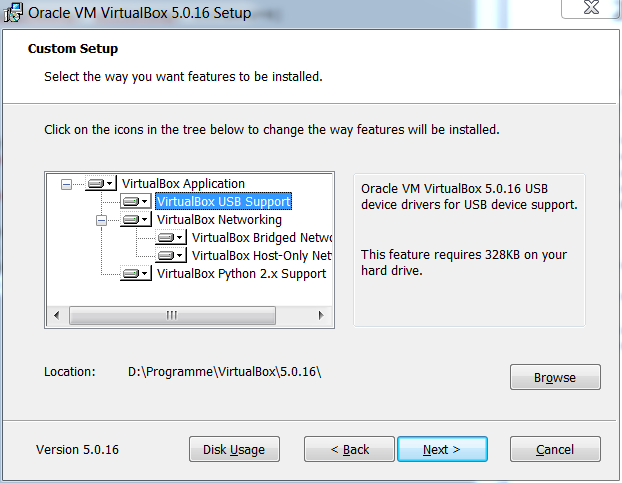
\includegraphics[scale=\screenshotscalefac]{Figures/VirtualBox_Install_Custom_Setup}
\end{figure}

During the installation simply answer the following questions with \textit{install} to allow access on the devices for the virtual machine.

\begin{figure}[htbp]
  \begin{subfigure}{\linewidth}
    \centering
    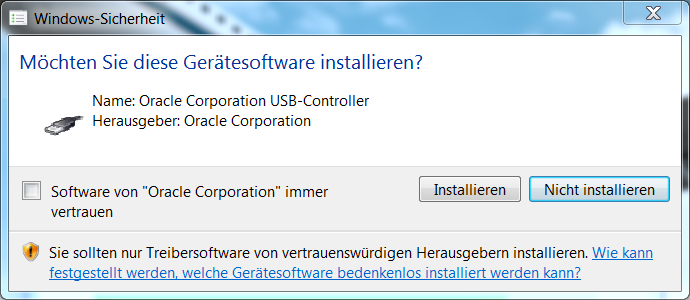
\includegraphics[scale=\screenshotscalefac]{Figures/VirtualBox_Install_Allow_USB}
    \caption{Install USB-Controller}
    \label{fig:VirtualBox_Install_Allow_USB}
  \end{subfigure}%
\vspace{1ex}\\
% \end{figure}
% 
% \begin{figure}[htbp]
%   \ContinuedFloat
  \begin{subfigure}{\linewidth}
    \centering
    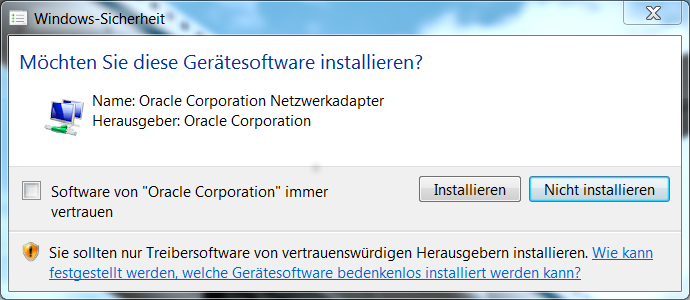
\includegraphics[scale=\screenshotscalefac]{Figures/VirtualBox_Install_Allow_Network_Adapter}
    \caption{Install network adapter}
    \label{fig:VirtualBox_Install_Allow_Network}
  \end{subfigure}%
  \vspace{1ex}\\
  \begin{subfigure}{\linewidth}
    \centering
    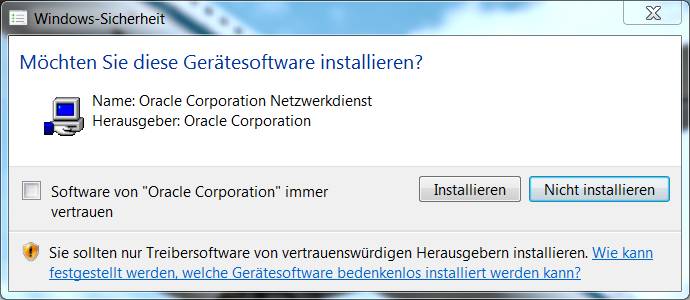
\includegraphics[scale=\screenshotscalefac]{Figures/VirtualBox_Install_Allow_Network_Service}
    \caption{Install network service}
   \label{fig:VirtualBox_Install_Allow_Network_Service}
  \end{subfigure}%
  \caption{Allow \marktool{\virtualboxname} access to devices}
  \label{fig:VirtualBox_Install_Allow}
\end{figure}

\clearpage

\levelstay{Create the virtual machine}

After the installation is complete start the \marktool{\virtualboxname} Manager.

\begin{figure}[htbp]
\centering
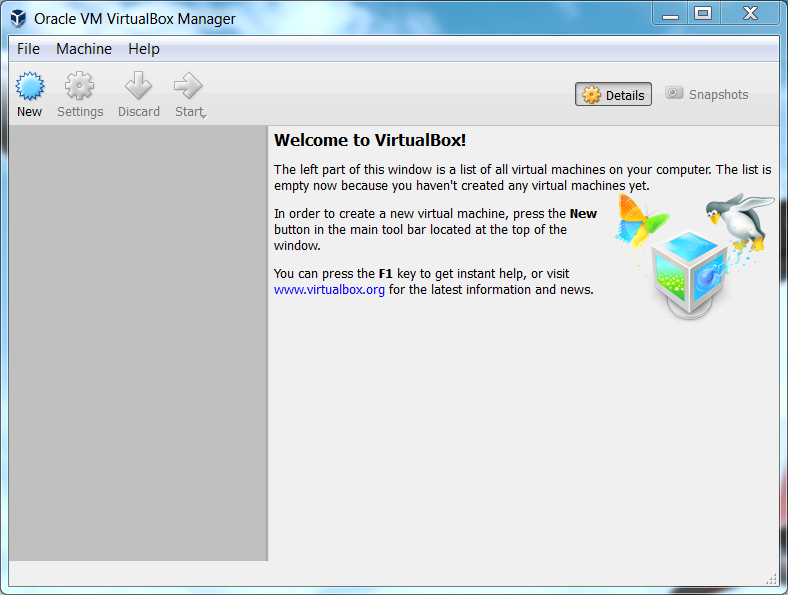
\includegraphics[scale=\screenshotscalefac]{Figures/VirtualBox_Start_Menu}
\end{figure}

Before we create a new virtual machine

\begin{itemize}[noitemsep]
 \item From the menu bar: Click \textit{File}
 \item Click \textit{Preferences}
 \item In the \textit{General} tab select the \textit{Default Machine Folder} to be a folder on a harddrive with sufficient amount of free memory to handle your virtual machine size, here 200GB\\
 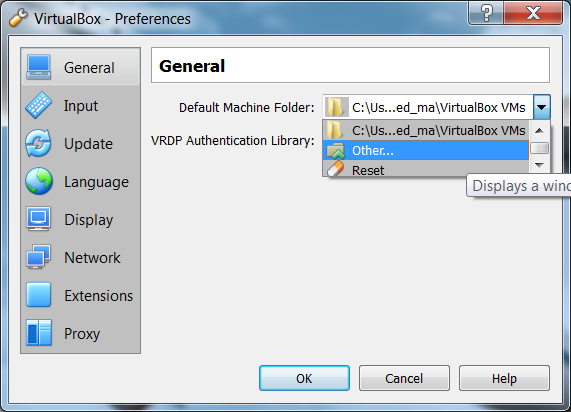
\includegraphics[scale=\screenshotscalefac]{Figures/VirtualBox_Preferences_General}
 \item Close the Preferences windows with a click in \textit{Ok}
\end{itemize}

Now we can create a new virtual machine. Click \textit{New} in the \marktool{\virtualboxname} Manager main window. A dialog appears that guides you through the setup of the virtual machine.

\begin{enumerate}[noitemsep]
  \item Select the virtual machine name, type and version
    \begin{itemize}
      \item Choose a name that includes the version \& the selection automatically jumps to your choice
      \item Choose the 64bit variant\\
      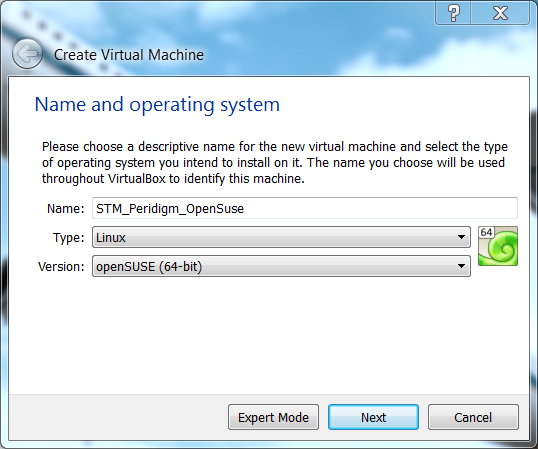
\includegraphics[scale=\screenshotscalefac]{Figures/VirtualBox_Create_VirtualMachine_Name_OS}
      \item A new folder with your chosen name is created in the directory you specified in the \textit{General} tab of the \textit{Preferences} toolbar menu
      \item Click \textit{Next}
    \end{itemize}
 \item Set the amount of RAM you grant your virtual machine
    \begin{itemize}
      \item The more RAM \marktool{\toolname} has available the better
      \item But your host operating system also still needs some RAM left to work with
      \item Choose an integer multiple of 1024 as amount of RAM
      \item Leave the host operating system at least 2GB of RAM
      \item You can select values in the red marked area\\
      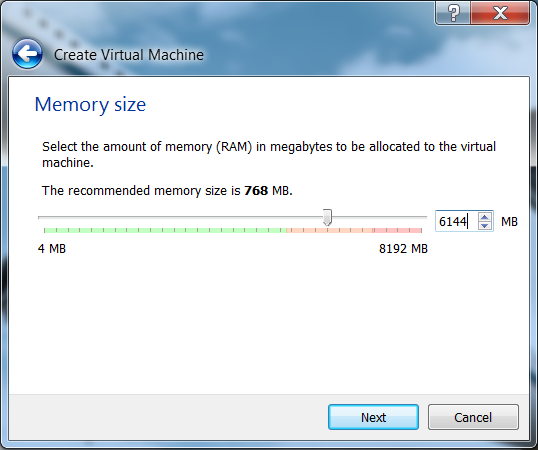
\includegraphics[scale=\screenshotscalefac]{Figures/VirtualBox_Create_VirtualMachine_RAM}
      \item Click \textit{Next}
    \end{itemize}
 \item Create a virtual hard disk to install your distribution on
    \begin{itemize}
      \item Here we select the \textit{Create a virtual hard disk now} option\\
      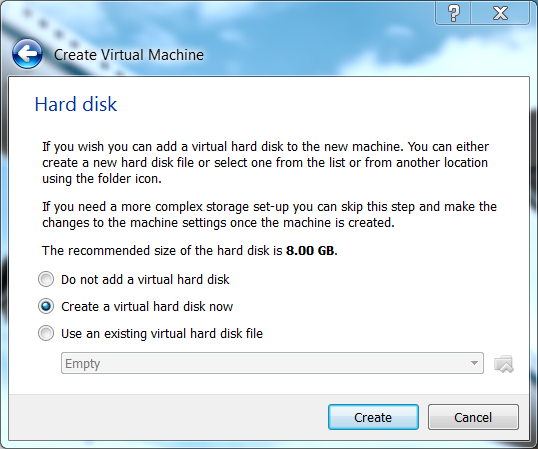
\includegraphics[scale=\screenshotscalefac]{Figures/VirtualBox_Create_VirtualMachine_Harddisk}
      \item Click \textit{Create}
      \item Select \textit{VMDK (Virtual Machine Disk)} to allow use of this virtual hard disk in other virtualization tools like VMWare.\\
      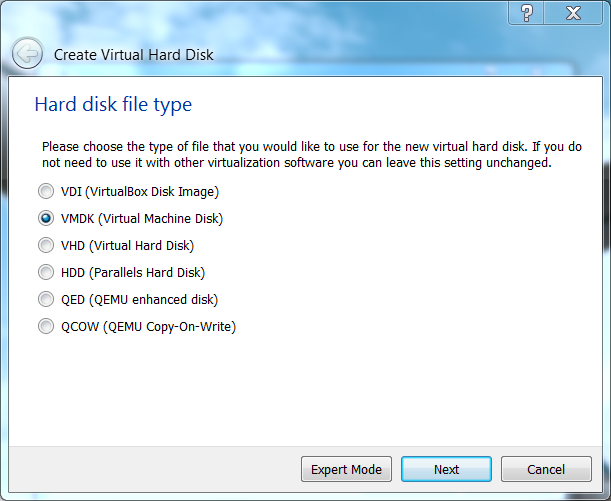
\includegraphics[scale=\screenshotscalefac]{Figures/VirtualBox_Create_VirtualMachine_Harddisk_File_Type}
      \item Click \textit{Next}
      \item Select \textit{Fixed size}
      \item Do not select \textit{Split into files less than 2GB}\\
      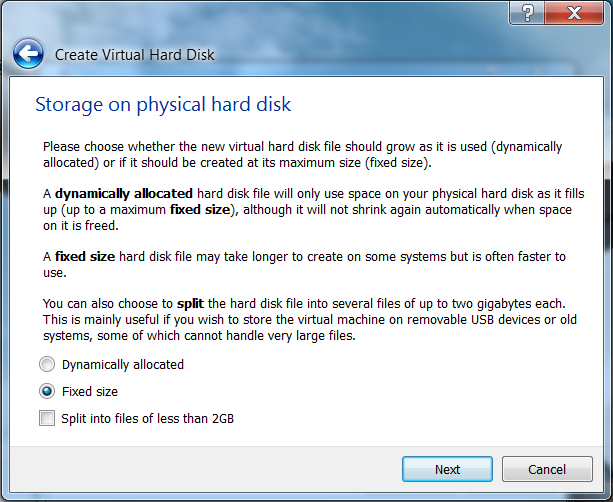
\includegraphics[scale=\screenshotscalefac]{Figures/VirtualBox_Create_VirtualMachine_Harddisk_Storage_Type}
      \item Click \textit{Next}
      \item Setup virtual hard disk name and size
      \item By default the name is identical to the virtual machine name
      \item If you click the folder button you can change the location of the virtual hard disk file. By default it is saved in your virtual machine folder in the directory specified in the \textit{General} tab of the \textit{Preferences} toolbar menu
      \item Set the size of the virtual hard disk to the amount you want and have free, here 200GB. Despite being saved in binary format, \marktool{\toolname} result files can be quite big and for explicit time integration a lot of them are created. Despite a Linux distribution does not need nearly as much hard disk space as a Windows installation, at least 120GB are proposed as virtual hard disk size.\\
      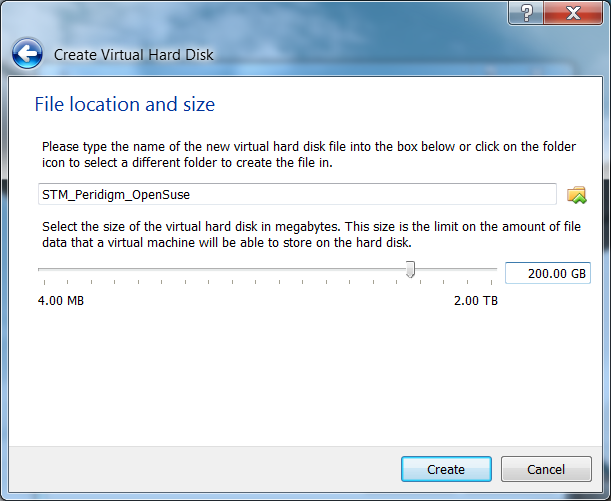
\includegraphics[scale=\screenshotscalefac]{Figures/VirtualBox_Create_VirtualMachine_Harddisk_Location}
      \item Click \textit{Create}
      \item Wait for the creation to finish
      \item Afterwards you have a new virtual machine\\
      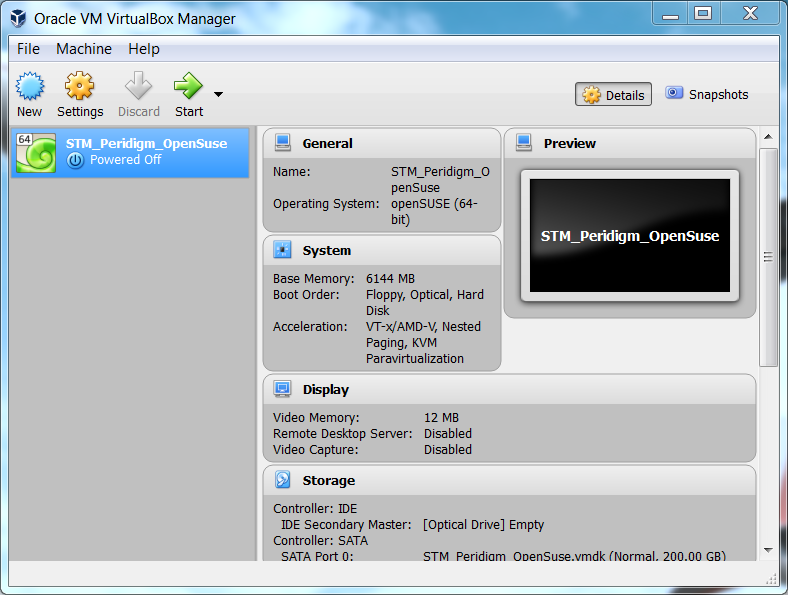
\includegraphics[scale=\screenshotscalefac]{Figures/VirtualBox_Create_VirtualMachine_Finished}
    \end{itemize}
  \item \label{enum:Virtual_Machine_Settings}Before we install the Linux distribution inside the virtual machine, we have to configure some settings
  \begin{itemize}
    \item Select the newly created virtual machine and click \textit{Settings}
    \item In the \textit{General} tab
    \begin{itemize}
      \item Select \textit{Advanced}
      \item Select:%\\
      \begin{tabular}[t]{ll}
      \textit{Shared Clipboard}	& Bidirectional	\\
      \textit{Drag'n'Drop}	& Bidirectional	\\
      \end{tabular}\\
      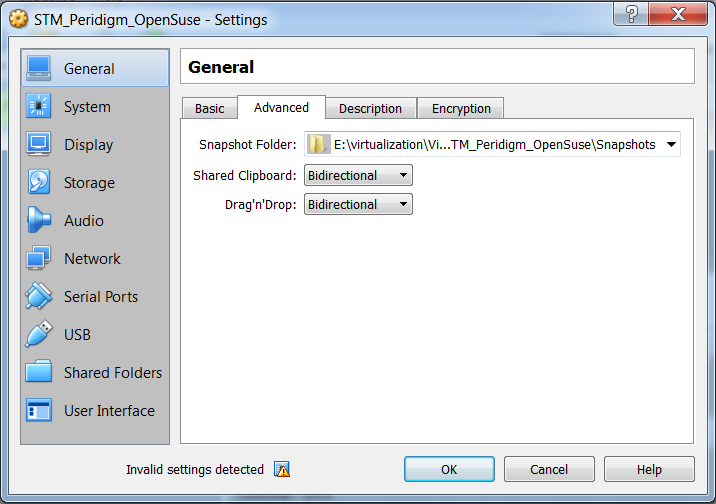
\includegraphics[scale=\screenshotscalefac]{Figures/VirtualBox_VirtualMachine_Settings_General_Advanced}
    \end{itemize}
    \item Ignore the warning about \textit{Invalid settings detected} if this is only a RAM issue
    \item In the \textit{System} tab
    \begin{itemize}
      \item Select \textit{Processor}
      \item Set \textit{Processor(s)} to your preferred value
      \item At least one CPU should be left for the host machine\\
      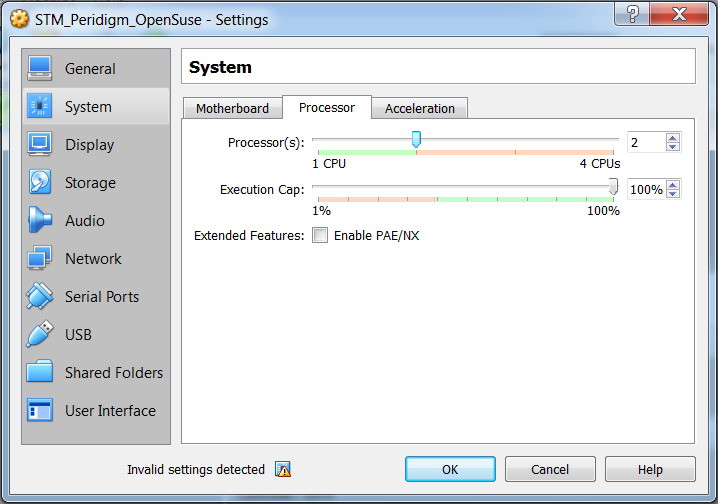
\includegraphics[scale=\screenshotscalefac]{Figures/VirtualBox_VirtualMachine_Settings_System_Processor}
    \end{itemize}
    \item In the \textit{Display} tab
    \begin{itemize}
      \item Select \textit{Screen}
      \item Set \textit{Video Memory} to maximum\\
      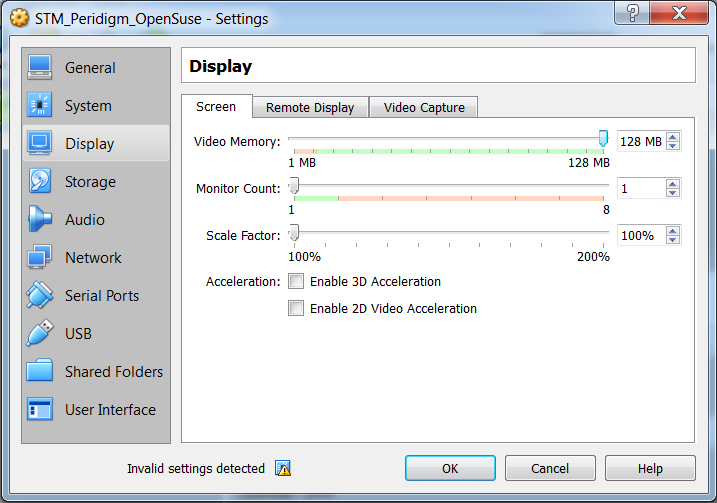
\includegraphics[scale=\screenshotscalefac]{Figures/VirtualBox_VirtualMachine_Settings_Display_Screen}
    \end{itemize}
%     \item In the \textit{Shared Folders} tab
%     \begin{itemize}
%       \item Click the + folder button on the right
%       \item In \textit{Folder Path:} create or add a transfer folder between your host system and your virtual machine\\
%       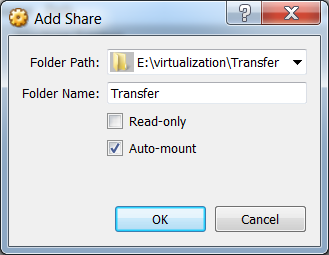
\includegraphics[scale=\screenshotscalefac]{Figures/VirtualBox_VirtualMachine_Settings_SharedFolders_Add}
%       \item Select \textit{Auto-mount}\\
%       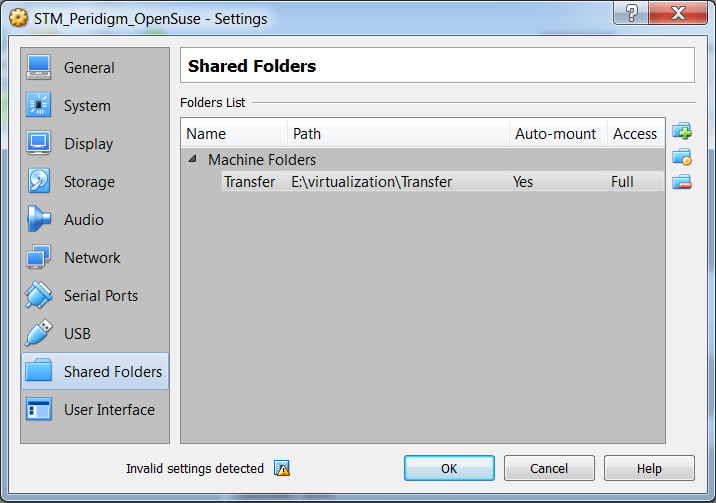
\includegraphics[scale=\screenshotscalefac]{Figures/VirtualBox_VirtualMachine_Settings_SharedFolders}
%     \end{itemize}
  \item Click \textit{OK}
  \end{itemize}
\end{enumerate}

All modifications to the virtual machine preferences in step \ref{enum:Virtual_Machine_Settings} can be modified after the installation of the virtual machine distribution in case the virtual machine is shut down.

\levelstay{Create a shared folder between host and virtual machine}



\begin{enumerate}[noitemsep]
  \item In the host operating system:
    \begin{itemize}
     \item Open a Windows Explorer
     \item Create a shared folder for the file exchange between the host and the virtual machine operating system anywhere it suits you or use an existing one, here the shared folder is \verb+E:\virtualization\Transfer+
     \item Right-Click the newly created folder and click \textit{Properties}
     \item In the \textit{Shared Folders/Freigabe} tab
      \begin{itemize}
	\item Click on \textit{Freigabe}
	\item In the dialog appearing click on the combobox arrow and select \textit{Anyone/Jeder}
	\item Click \textit{Freigabe}
	\item Click \textit{Close}
      \end{itemize}
      \item Be aware that the folder is visible in your whole network
    \end{itemize}
  \item Inside the virtual box manager:
    \begin{itemize}
      \item Select the newly created virtual machine and click \textit{Settings}
      \item In the \textit{Shared Folders} tab
      \begin{itemize}
	\item Click the + folder button on the right
	\item In \textit{Folder Path:} create or add a transfer folder between your host system and your virtual machine\\
	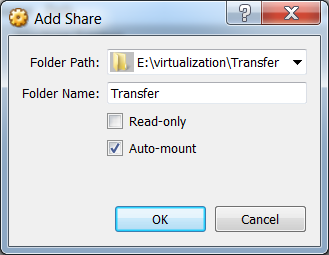
\includegraphics[scale=\screenshotscalefac]{Figures/VirtualBox_VirtualMachine_Settings_SharedFolders_Add}
	\item Select \textit{Auto-mount}\\
	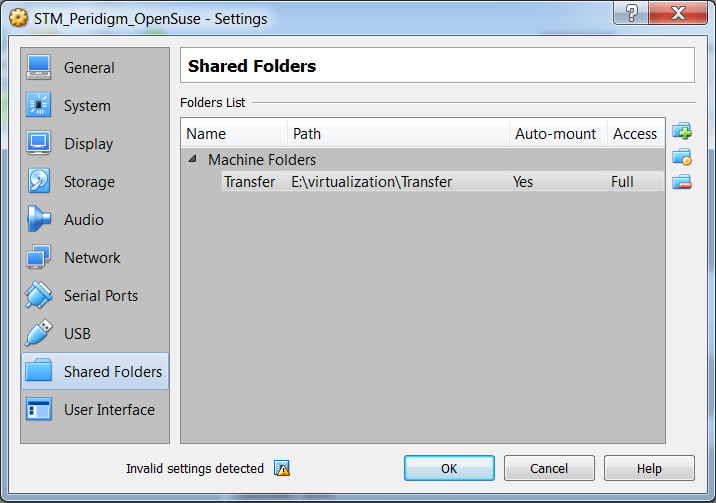
\includegraphics[scale=\screenshotscalefac]{Figures/VirtualBox_VirtualMachine_Settings_SharedFolders}
      \end{itemize}
    \item Click \textit{OK}
    \end{itemize}
\end{enumerate}

\levelstay{Install the operating system in the virtual machine}

Now, we can install the virtual machine operating system:

\begin{enumerate}[noitemsep]
 \item Start the installation
 \begin{itemize}
   \item Select the virtual machine in the \marktool{\virtualboxname} Manager and click \textit{Start}\\
   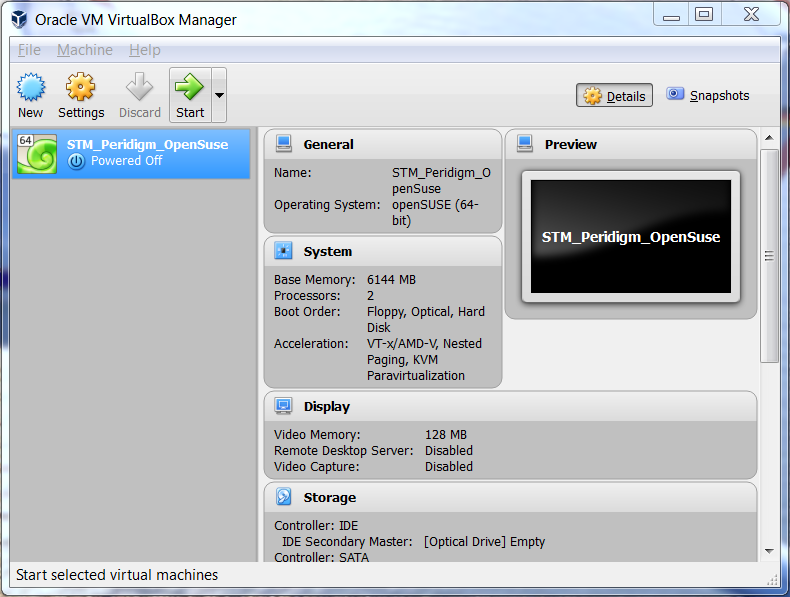
\includegraphics[scale=\screenshotscalefac]{Figures/VirtualBox_VirtualMachine_OperatingSystem_Start}
   \item Select the \marktool{\opensusename} image from section \ref{sec:VirtualBox_Download_Linux_Distribution}\\
   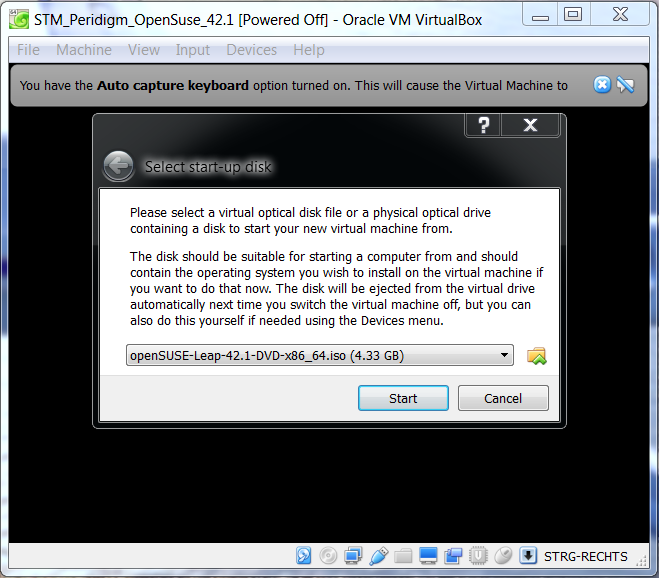
\includegraphics[scale=\screenshotscalefac]{Figures/VirtualBox_VirtualMachine_OperatingSystem_SelectDisk}
   \item Click \textit{Start}
 \end{itemize}
 \item Setup the installation
 \begin{itemize}
   \item In the \marktool{\opensusename} boot menu select \textit{Installation}\\
   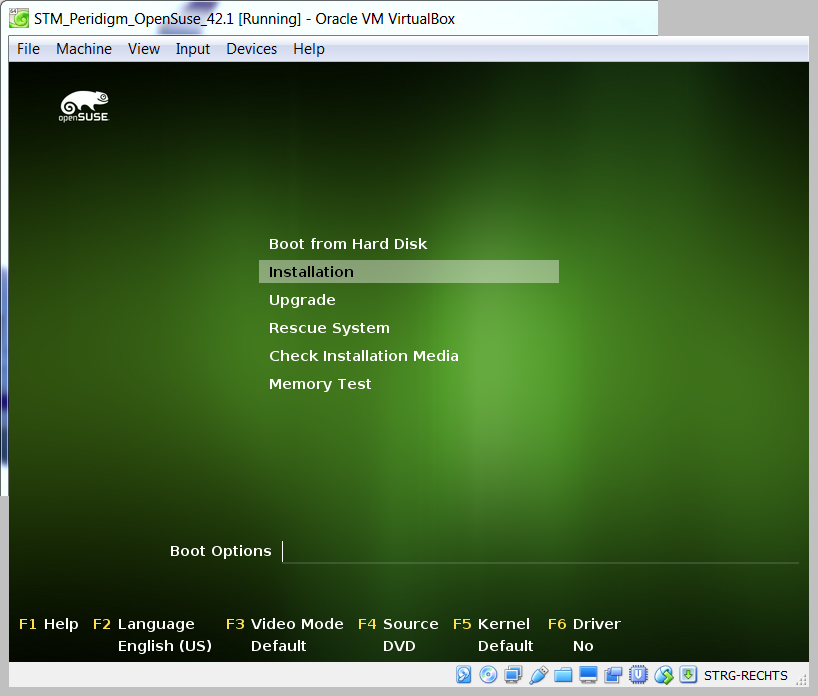
\includegraphics[scale=0.25]{Figures/VirtualBox_VirtualMachine_OperatingSystem_Boot_Installation}
   \item Set the Language and Keyboard layout to your preferred option\\
   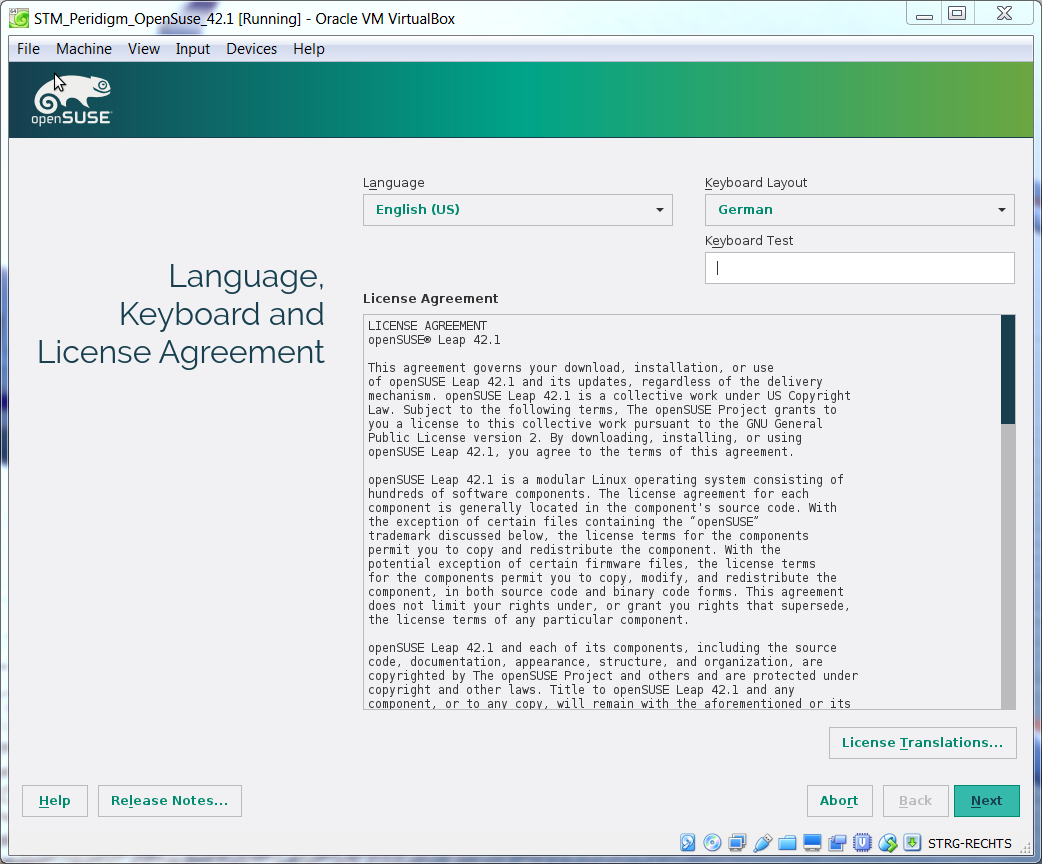
\includegraphics[scale=0.25]{Figures/VirtualBox_VirtualMachine_OperatingSystem_Language}
   \item Click \textit{Next}
   \item In the \textit{Installation Options} to not toggle on any of the options\\
   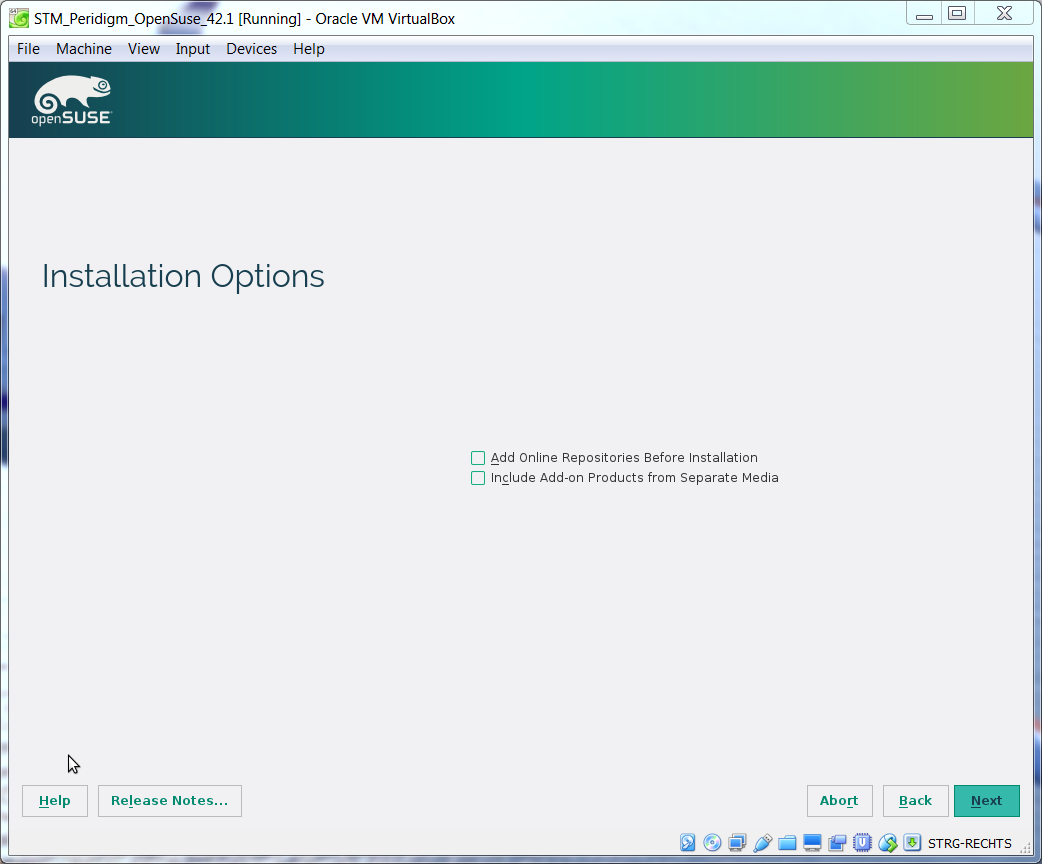
\includegraphics[scale=0.25]{Figures/VirtualBox_VirtualMachine_OperatingSystem_InstallationOptions}
   \item Click \textit{Next}
   \item Use the \textit{Suggested Partition} and click \textit{Next}
   \item Click on the Map to select your country to set \textit{Clock and Time Zone} and click \textit{Next}
   \item Use \textit{KDE Desktop} in \textit{Desktop Selection} and click \textit{Next}\\
   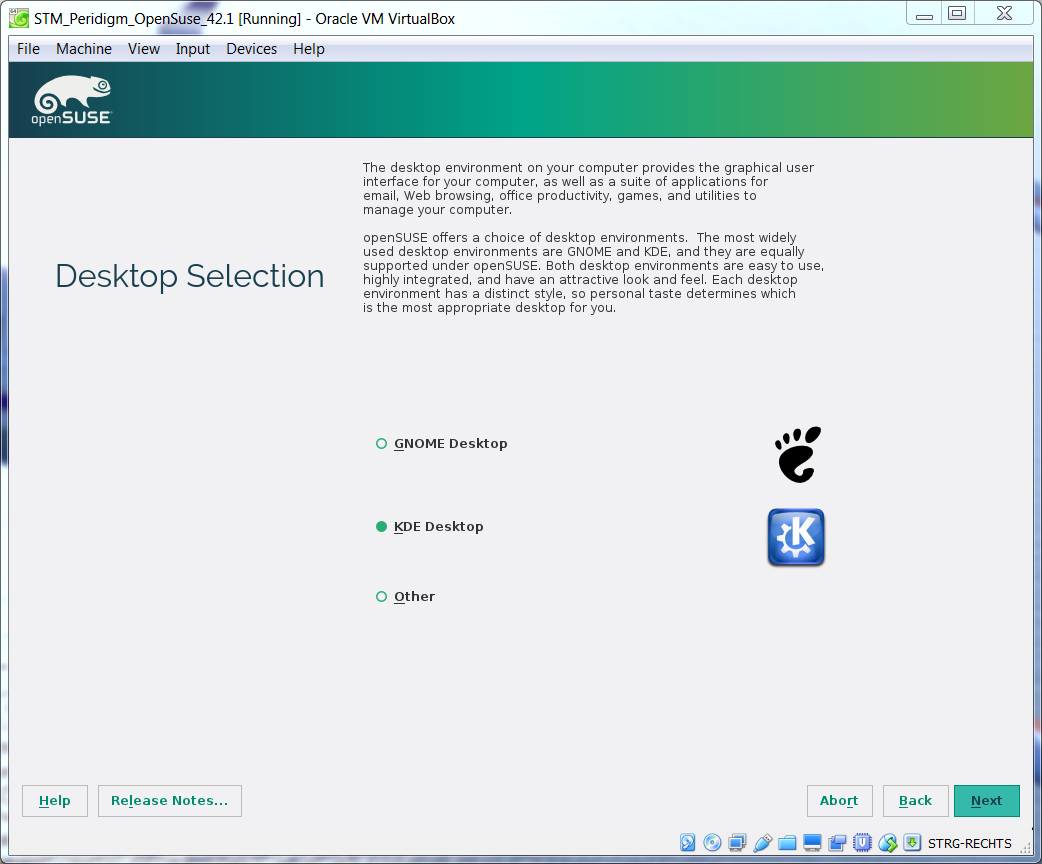
\includegraphics[scale=0.25]{Figures/VirtualBox_VirtualMachine_OperatingSystem_DesktopSelection}
   \item Setup the first user name \& password
   \begin{itemize}
    \item You can use the same user and root password if you are and will always be the only user of your virtual machine
    \item User: 
      \begin{tabular}[t]{ll}
      \textit{Username}	& stm	\\
      \textit{Password}	& 13112	\\
      \end{tabular}
    \item Admin:
      \begin{tabular}[t]{ll}
      \textit{Password}	& dlr-fa-13112-bs	\\
      \end{tabular}
    \item Click next
   \end{itemize}
   \item In the next windows click \textit{Install}
 \end{itemize}
 \item After installation
 \begin{itemize}
   \item After the installation is complete virtual system restarts. Now select \textit{Boot from Hard Disk}\\
   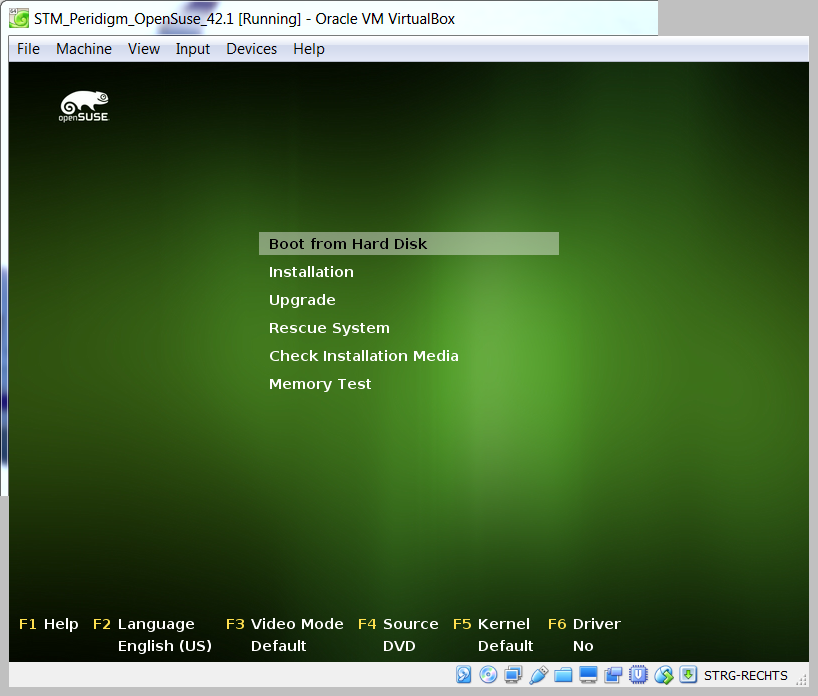
\includegraphics[scale=0.25]{Figures/VirtualBox_VirtualMachine_OperatingSystem_Boot_HardDisk}
   \item Select the normal version and press Enter\\
   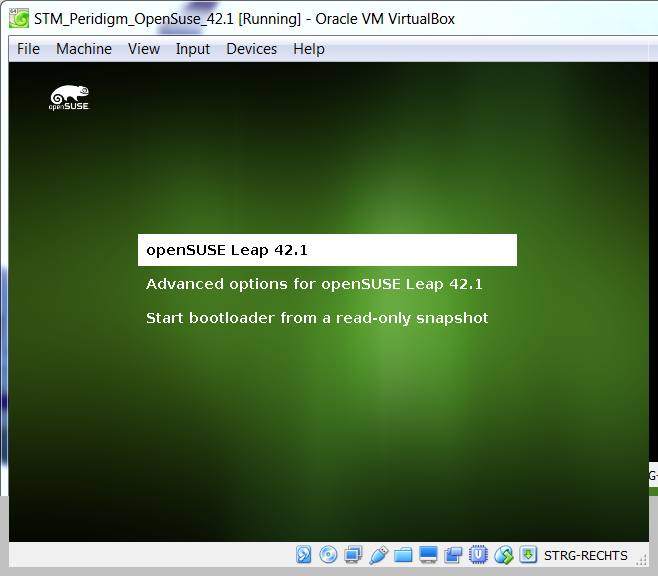
\includegraphics[scale=0.25]{Figures/VirtualBox_VirtualMachine_OperatingSystem_Boot_Version}
   \item Login with your password\\
   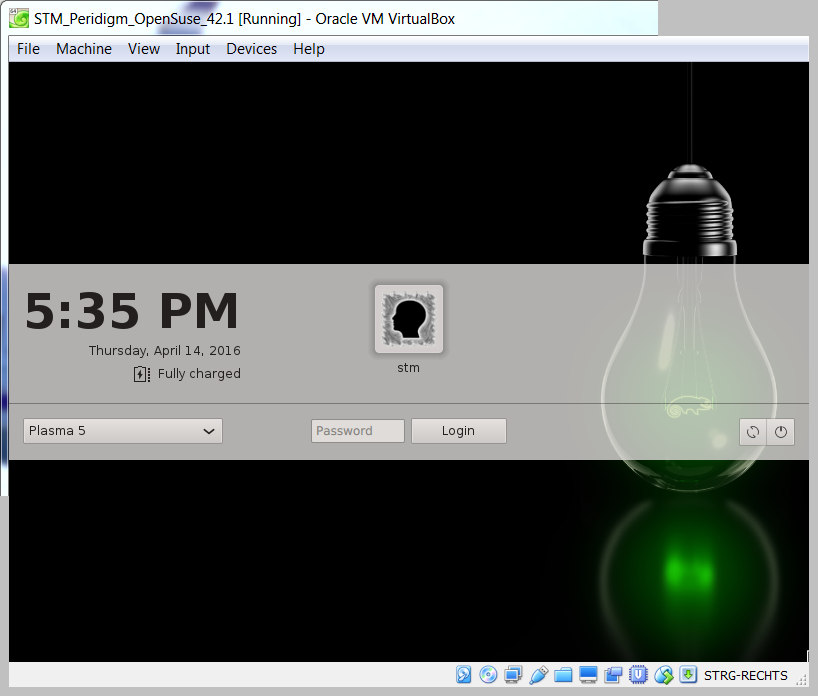
\includegraphics[scale=0.25]{Figures/VirtualBox_VirtualMachine_OperatingSystem_Login}
   \item Open a shell
   \item Login as root user, perform
\begin{code}
zypper refresh
zypper update
\end{code}
   And select yes to perform an operating system update
   \item Restart the virtual machine operating system
 \end{itemize}
\end{enumerate}

Ta-daa you have a linux installation inside of a virtual machine.

\levelstay{User modifications to use shared folders}

In order for the Linux users to use the virtual machine shared folders

\begin{enumerate}[noitemsep]
 \item Open \marktool{\yastname}
 \item In the \textit{Security and Users} tab open {User and Group Management}
 \item Select the user and click \textit{Edit}
 \item Go to \textit{Details} tab
 \item On the right select \textit{users} and \textit{vboxsf} as \textit{Additional Groups} and click \textit{OK}
 \item Restart your virtual system
\end{enumerate}

The shared folders are mounted under \verb+/media/+. In the current case the single shared folder is accessible under \verb+/media/sf_transfer/+ .

\levelstay{Save the virtual machine state}

After the operating system installation it is recommended to save a snapshot of the current virtual machine state. Thus, it is always possible to reset your virtual machine to this state in case anything goes wrong during the \marktool{\toolname} installation.

To create a snapshot:

\begin{enumerate}[noitemsep]
 \item Open the \marktool{\virtualboxname} Manager
 \item In the upper right corner select \textit{Snapshots}
 \item Click the little camera button to take a snapshot of the current virtual machine state\\
 \begin{tikzpicture}
   % External figure
   \node[anchor=south west,inner sep=0] (image) at (0,0){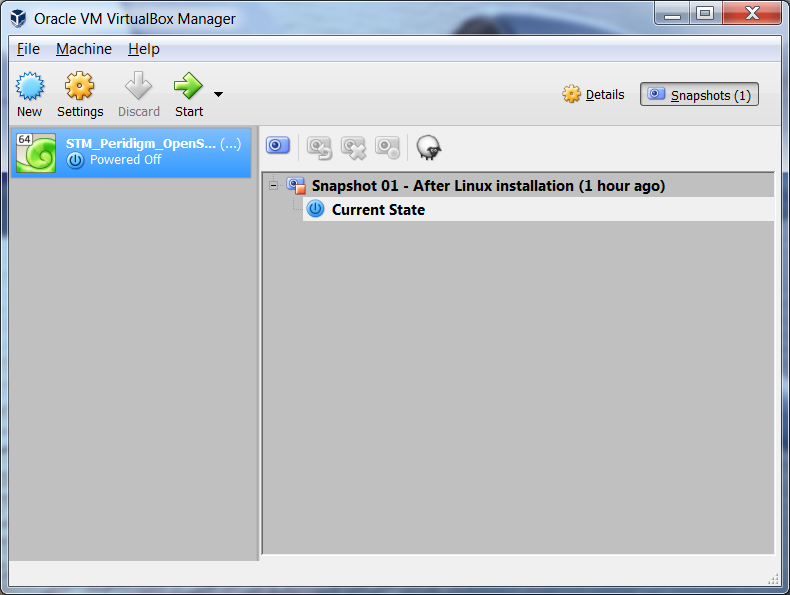
\includegraphics[scale=\screenshotscalefac]{Figures/VirtualBox_VirtualMachine_Snapshot}};
   % Figure scope
   \begin{scope}[
     x={(image.south east)},
     y={(image.north west)},
   ]
     % Red rectangle
     \draw[red,ultra thick,rounded corners] (0.325,0.73) rectangle (0.3775,0.786);
     % Help grid and labels
%      \pic{myimagegrid};
   \end{scope}
 \end{tikzpicture}
 
\end{enumerate}


\chapter{\texorpdfstring{\protect\marktool{\toolnameshort}}{\toolnameshort{}} Linux installation}
\label{sec:Peridigm_Linux_Installation}
\setcounter{currentlevel}{6}
%%%%%%%%%%%%%%%%%%%%%%%%%%%%%%%%%%%%
% Header                           %
%%%%%%%%%%%%%%%%%%%%%%%%%%%%%%%%%%%%
% 
% Revisions: 2017-04-10 Martin Rädel <martin.raedel@dlr.de>
%                       Initial draft
%               
% Contact:   Martin Rädel,  martin.raedel@dlr.de
%            DLR Composite Structures and Adaptive Systems
%          
%                                 __/|__
%                                /_/_/_/  
%            www.dlr.de/fa/en      |/ DLR
% 
%%%%%%%%%%%%%%%%%%%%%%%%%%%%%%%%%%%%
% Content                          %
%%%%%%%%%%%%%%%%%%%%%%%%%%%%%%%%%%%%

\leveldown{Tested combinations}

\leveldown{CPU-Architecture \& operating system}

\leveldown{System 1 - STM-Laptop}

\begingroup
\renewcommand{\arraystretch}{1.2}
\begin{tabularx}{\linewidth}{@{}lllX}
Hardware:	& CPU:	& Name:		& Intel Core i7 M620	\\
		&	& Architecture:	& x86\_64		\\
		&	& Cores:	& 4			\\
		&	& Threads:	& 4			\\
		&	& Clock rate:	& 2.67GHz		\\
		& RAM:	& Amount:	& 8Gb			\\[0.5ex]
Software:	& OS:	& Name:		& openSUSE		\\
		&	& Version:	& 42.1			\\
		&	& Type:		& 64bit
\end{tabularx}
\endgroup

\levelstay{System 2 - Virtual machine}

\begingroup
\renewcommand{\arraystretch}{1.2}
\begin{tabularx}{\linewidth}{@{}llllX}
Hardware:	& Host:	& CPU:	& Name:		& Intel Core i7-4600U	\\
		&	&	& Architecture:	& x86\_64		\\
		&	&	& Cores:	& 2			\\
		&	&	& Threads:	& 4			\\
		&	&	& Clock rate:	& 2.1GHz		\\
		&	& RAM:	& Amount:	& 8Gb			\\[0.5ex]
		& VM:	& CPU:	& Cores:	& 2			\\
		&	& RAM:	& Amount:	& 6Gb			\\[0.5ex]
Software:	& Host:	&	&		& VirtualBox 5.0	\\ 
		& VM:	& OS:	& Name:		& openSUSE		\\
		&	&	& Version:	& 42.1			\\
		&	&	& Type:		& 64bit
\end{tabularx}
\endgroup

\levelstay{System 3 - STM-Cluster}

\begingroup
\renewcommand{\arraystretch}{1.2}
\begin{tabularx}{\linewidth}{@{}lllX}
Hardware:	& CPU:	& Name:		& Intel Xeon E5-2407	\\
		&	& Architecture:	& x86\_64		\\
		&	& Number:	& 8			\\
		&	& Cores:	& 4			\\
		&	& Threads:	& 4			\\
		&	& Clock rate:	& 2.2GHz		\\
		& RAM:	& Amount:	& 32Gb			\\[0.5ex]
Software:	& OS:	& Name:		& SUSE Linux Enterprise Server	\\
		&	& Version:	& 11			\\
		&	& Patchlevel:	& 3			\\
		&	& Type:		& 64bit
\end{tabularx}
\endgroup

\levelup{Library and system combinations}

\begingroup
\renewcommand{\arraystretch}{1.1}
\begin{tabularx}{\linewidth}{cllYYYY}
\toprule
& \multicolumn{2}{l}{Setup}					& 1			& 2			& 3			& 4		\\
\midrule
& \multicolumn{2}{l}{System}					& STM-Laptop		& VirtualBox		& VirtualBox		& STM-Cluster	\\[2ex]
\multirow{7}{*}{\rotatebox{90}{Basics}}
& Compiler	& Fortran					& gcc-fortran 4.8.5	& gcc-fortran 4.8.5	& gcc-fortran 4.8.5	& gcc-fortran 4.8.5	\\
&	 	& C						& gcc 4.8.5		& gcc 4.8.5		& gcc 4.8.5		& gcc 4.8.5	\\
&	 	& \Cpp						& gcc-c++ 4.8.5		& gcc-c++ 4.8.5		& gcc-c++ 4.8.5		& gcc-c++ 4.8.5	\\
& \multicolumn{2}{l}{\marktool[\cmakeaddress]{\cmakename}}	& 3.4.3			& 3.4.3			& 3.5.1			& 3.5.2		\\
& \marktool{MPI}& \marktool[\openmpiaddress]{\openmpiname}	& 1.10.2		& 1.10.2		& 1.10.2		& 1.10.4	\\
& 		& \marktool[\mpichaddress]{\mpichname}		& -			& -			& -			& -		\\
& \multicolumn{2}{l}{\marktool[\pythonaddress]{\pythonname}}	& 2.7.11		& 2.7.9			& 2.7.9			& 2.6.9		\\[2ex]
\multirow{4}{*}{\rotatebox{90}{Libraries}}
& \multicolumn{2}{l}{\marktool[\boostaddress]{\boostname}}	& 1.55.0		& 1.55.0		& 1.60.0		& ?		\\
& \multicolumn{2}{l}{\marktool[\hdfaddress]{\hdfname}}		& 1.8.16		& 1.8.16		& 1.10.0		& ?		\\
& \multicolumn{2}{l}{\marktool[\netcdfaddress]{\netcdfname}}	& 4.4.0			& 4.4.0			& 4.4.0			& 4.4.1		\\
& \multicolumn{2}{l}{\marktool[\trilinosaddress]{\trilinosname}}& 12.4.2		& 12.4.2		& 12.6.1		& ?		\\[2ex]
& \multicolumn{2}{l}{\marktool[\tooladdress]{\toolname}}	& 1.4.1			& 1.4.1			& 1.5.0			& 1.4.1\\
\bottomrule
\end{tabularx}
\endgroup

\newpage
\section{Basics}
\setcounter{currentlevel}{5}

The following section describes the installation of the required basic packages for the \marktool[\tooladdress]{\toolnameshort} libraries. The subsections are in the order required for a proper installation.

%%%%%%%%%%%%%%%%%%%%%%%%%%%%%%%%%%%%
% Header                           %
%%%%%%%%%%%%%%%%%%%%%%%%%%%%%%%%%%%%
% 
% Revisions: 2017-04-10 Martin Rädel <martin.raedel@dlr.de>
%                       Initial draft
%               
% Contact:   Martin Rädel,  martin.raedel@dlr.de
%            DLR Composite Structures and Adaptive Systems
%          
%                                 __/|__
%                                /_/_/_/  
%            www.dlr.de/fa/en      |/ DLR
% 
%%%%%%%%%%%%%%%%%%%%%%%%%%%%%%%%%%%%
% Content                          %
%%%%%%%%%%%%%%%%%%%%%%%%%%%%%%%%%%%%

\leveldown{Preliminary remarks}

\leveldown{Installation shell}

The following description is valid for an installation using the \verb+bash+ as shell. If you use any other shell, e.g. \verb+ksh+, \verb+csh+ or their decendants you have to modify the environment variable parts of this guide or simply type \verb+bash+ and Enter in your \verb+tcsh+ to switch shells.

\levelstay{Download directories}

During the course of this installation guide it will be necessary to download several source code packages. In the instructions the key \colorbox{verbgray}{\lstinline[style=inlinetexstyle]+$DOWNLOAD_DIR+} is the identifier for the download directory. The scripts in the appendix of this documents assume that

\begin{code}
$DOWNLOAD_DIR=/usr/local/src/
\end{code}

You are free to choose any other folder as the download directory. If you do so, you have to modify the source code path in the scripts in the appendix accordingly.

\levelstay{\texttt{PATH} variable for user defined installation directories}

It is assumed that the current installations are performed for all users of the device. Thus, the global installation directory \verb+/usr/bin/+ is used.

However, the installation directory for each tool can be changed, e.g. with

\begin{code}
./configure --prefix="/home/$USER/TOOL"
\end{code}

If this is done, the path to the executables have to exported to the \verb+PATH+ variables.

\begin{code}
export PATH="$PATH:/home/$USER/TOOL/bin"
export LD_LIBRARY_PATH="$LD_LIBRARY_PATH:/home/$USER/TOOL/lib/"
\end{code}

This has to performed for each individual installation directory.

\textcolor{red}{NEVER EVER FORGET THE \texttt{\$PATH:} AND \texttt{\$LD\_LIBRARY\_PATH:} IN THE BEGINNING OR A NEW EMPTY PATH VARIABLE WILL BE CREATED AND ADDED TO. YOU WILL NOT BE ABLE TO USE ANYTHING USEFUL ON YOUR DEVICE BECAUSE ALL ALIASES WILL BE DELETED.}

\levelstay{Installation user}

All installations are performed as \verb+root+ user. To make sure that the end user is allowed to use the installed programs make sure that they have the necessary permissions. The default installation directory for installations with a package manager or \marktool{\zyppername} is \verb+/usr/bin+. You can check if the permissions are correct by opening a terminal, navigation to \verb+/usr/bin+ and the command

\begin{code}
ls -l | grep PARTOFTOOLABBREVIATION
\end{code}

For \verb+ls -l | grep gcc+ the result might look something like this:

\begingroup
\lstset{keepspaces=true}
\begin{code}
lrwxrwxrwx 1 root root      7  5. Feb 14:07 cc -> gcc-4.8
lrwxrwxrwx 1 root root      7  5. Feb 14:07 gcc -> gcc-4.8
-rwxr-xr-x 1 root root 755680 29. Okt 18:02 gcc-4.8
lrwxrwxrwx 1 root root     10  5. Feb 14:07 gcc-ar -> gcc-ar-4.8
-rwxr-xr-x 1 root root  27136 29. Okt 18:02 gcc-ar-4.8
lrwxrwxrwx 1 root root     10  5. Feb 14:07 gcc-nm -> gcc-nm-4.8
-rwxr-xr-x 1 root root  27136 29. Okt 18:02 gcc-nm-4.8
lrwxrwxrwx 1 root root     14  5. Feb 14:07 gcc-ranlib -> gcc-ranlib-4.8
-rwxr-xr-x 1 root root  27144 29. Okt 18:02 gcc-ranlib-4.8
\end{code}
\endgroup

In the first column the current rights are specified. The first symbol shows if the current entry is a link or not. The nine symbol afterwards are the three individual rights for user, group and other. The three individual rights are r-read, w-write and x-execute.

If the permissions are not set correctly, consult the documentation of \marktool{chmod}. 
%%%%%%%%%%%%%%%%%%%%%%%%%%%%%%%%%%%%
% Header                           %
%%%%%%%%%%%%%%%%%%%%%%%%%%%%%%%%%%%%
% 
% Revisions: 2017-04-10 Martin Rädel <martin.raedel@dlr.de>
%                       Initial draft
%               
% Contact:   Martin Rädel,  martin.raedel@dlr.de
%            DLR Composite Structures and Adaptive Systems
%          
%                                 __/|__
%                                /_/_/_/  
%            www.dlr.de/fa/en      |/ DLR
% 
%%%%%%%%%%%%%%%%%%%%%%%%%%%%%%%%%%%%
% Content                          %
%%%%%%%%%%%%%%%%%%%%%%%%%%%%%%%%%%%%

\levelup{Root .bashrc file}

You usually login as a normal user to \marktool{\opensusename} but changes to the system are performed as root user.

During this installation guide modifications of the .bashrc, a hidden file in the user home directory are requested. For the installation process as root user it is necessary that these modifications also take effect for the root user.

To achieve this a symbolic link is created in the root home directory to the modified .bashrc in the ordinary user directory. To achieve this open a console and perform the following steps

\begin{code}
su %\lstcomment{\# Switch to root user}%
cd %\lstcomment{\# Change to root home}%
ln -sf /home/$USERNAME/.bashrc . %\lstcomment{\# Create symbolic link}%
\end{code}

This way, the root .bashrc file is always an identical copy of the one of the user with the name \verb+$USERNAME+ here.
%%%%%%%%%%%%%%%%%%%%%%%%%%%%%%%%%%%%
% Header                           %
%%%%%%%%%%%%%%%%%%%%%%%%%%%%%%%%%%%%
% 
% Revisions: 2017-04-10 Martin Rädel <martin.raedel@dlr.de>
%                       Initial draft
%               
% Contact:   Martin Rädel,  martin.raedel@dlr.de
%            DLR Composite Structures and Adaptive Systems
%          
%                                 __/|__
%                                /_/_/_/  
%            www.dlr.de/fa/en      |/ DLR
% 
%%%%%%%%%%%%%%%%%%%%%%%%%%%%%%%%%%%%
% Content                          %
%%%%%%%%%%%%%%%%%%%%%%%%%%%%%%%%%%%%

\levelstay{Fortran \& C \& \texorpdfstring{\protect\Cpp{}}{\Cpp{}}-compiler}

\marktool[\tooladdress]{\toolnameshort} as well as \marktool{\pythonname} python require an acceptable C or \Cpp-compiler. \marktool{\trilinosname} additionally needs a Fortran-compiler. Here, the free \marktool[\gccaddress]{GNU Compiler Collection} versions, short \marktool{\gccname} are used. The current release and further informations can be found on

\href{\gccaddress}{\gccaddress}

Currently, there are two main versions available, \marktool{\gccname}, which is basically \marktool{\gccname} version 4.8, as well as \marktool{\gccname5}. The installation of the used \marktool{\pythonname} currently seems not to work with \marktool{\gccname5}. Additionally, \marktool{\trilinosname} needs a compiler that is \verb|C++11| compliant and thus needs \marktool{\gccname} version \textbf{4.7.2 or later}. Therefore \marktool{\gccname} version 4.8 is used. If using Intel compilers, version 13 or later is required by \marktool{\trilinosname}.

Normally, the \marktool[\gccaddress]{\gccname} repository is already part of an \marktool[\opensuseaddress]{\opensusename} distribution. To check the availability of the \marktool[\gccaddress]{\gccname}-repository in your \marktool[\opensuseaddress]{\opensusename} distribution open a terminal as root and use the following command to get a list of all repositories.

\begin{code}
zypper repos
\end{code}

\paragraph{Installation with \marktool{\yastname}}

To install the Fortran-, C- and \Cpp-compilers of \marktool[\gccaddress]{\gccname} with the package manager perform the following steps:

\begin{enumerate}[itemsep=-1.5ex]
 \item Open \marktool{\yastname}
 \item Click on \textit{Install software}
 \item Go to the \textit{Search} tab
 \item Search for \gccname
 \item Check \marktool{gcc-fortran}, \marktool{gcc} and \marktool{gcc-c++}
 \item Click on apply
\end{enumerate}

\paragraph{Installation from source}

ToDo

\paragraph{Installation with \marktool{\opensusename}-repository}

To use \marktool{\zyppername} open a terminal as root. Use the following commands to install Fortran-, C- and \Cpp-compilers of \marktool[\gccaddress]{\gccname} from the repositories. Answer the questions if installation shall continue with yes.

\begin{code}
zypper install gcc-fortran
zypper install gcc
zypper install gcc-c++
\end{code}

The installation usually is performed to \verb+/usr/bin/+. If another installation directory is used, it has to be made sure, that this directory is part of the \verb+$PATH+-variable. To check if this is the case, open a terminal type

\begin{code}
echo $PATH
\end{code}

The installation directory has to be an entry of the printed string.
%%%%%%%%%%%%%%%%%%%%%%%%%%%%%%%%%%%%
% Header                           %
%%%%%%%%%%%%%%%%%%%%%%%%%%%%%%%%%%%%
% 
% Revisions: 2017-04-10 Martin Rädel <martin.raedel@dlr.de>
%                       Initial draft
%               
% Contact:   Martin Rädel,  martin.raedel@dlr.de
%            DLR Composite Structures and Adaptive Systems
%          
%                                 __/|__
%                                /_/_/_/  
%            www.dlr.de/fa/en      |/ DLR
% 
%%%%%%%%%%%%%%%%%%%%%%%%%%%%%%%%%%%%
% Content                          %
%%%%%%%%%%%%%%%%%%%%%%%%%%%%%%%%%%%%

\levelstay{\texorpdfstring{\protect\marktool{\cmakename}}{\cmakename{}}}

\marktool{\cmakename} is cross-platform free and open-source software for managing the build process of software using a compiler-independent method. It is maintained by Kitware. The official homepage of is \marktool{\cmakename}

\href{https://cmake.org/}{https://cmake.org/}

\marktool{\trilinosname} release 12.4 and higher use a \marktool{\cmakename} build system, which requires \marktool{\cmakename} version \textbf{2.8.11 or newer}.

\paragraph{Installation from source}

In order to install \marktool{\cmakename} from the official or any other binary source open a terminal and login as root. Change directory to the designated download folder, e.g. \verb+/usr/local/src/+ and perform the following steps:

\begin{code}
cd $DOWNLOAD_DIR
wget http://www.cmake.org/files/v3.4/cmake-3.4.3.tar.gz	%\lstcomment{\# Download}%
tar xvfz cmake-3.4.3.tar.gz 	%\lstcomment{\# unzip}%
cd cmake-3.4.3			%\lstcomment{\# go into directory}%
./configure --prefix=/usr/local/bin/cmake-3.4.3 > configure_cmake.log 2>&1
make > make_cmake.log 2>&1		%\lstcomment{\# build}%
make install > make_install_cmake.log 2>&1 %\lstcomment{\# install}%
\end{code}

If you want to see the available configuration options, run the command below in the terminal.

\begin{code}
./configure --help
\end{code}

In order to configure the installation directory of \marktool{\cmakename} before installation, run the command below

\begin{code}
./configure --prefix=/opt/cmake
\end{code}

After installation without any errors you can verify the installation by running the command below:

\begin{code}
/usr/local/bin/cmake-3.4.3/bin/cmake -version
\end{code}

The output should look something like below (depending upon \marktool{\cmakename} version you are installing).

\begin{code}
cmake version 3.4.3
\end{code}

Afterwards, the \marktool{\cmakename}-directory has to be added to the \verb+PATH+ environment variable

\begingroup
\lstset{breaklines = true}
\lstinputlisting[
  style=scriptstyle,
  linerange={37-37},
  nolol,
  ]{Scripts/modified_bashrc.txt}
\endgroup

\paragraph{Installation with \texorpdfstring{\protect\marktool{\opensusename}}{\opensusename{}}-repository}

For the installation of the build process manager \marktool{\zyppername} visit:

\href{http://software.opensuse.org/download.html?project=server\%3Airc\&package=cmake}{http://software.opensuse.org/download.html?project=server\%3Airc\&package=cmake}

You can either choose the 1-Click-installation or add the repository and install manually. For the latter login to a terminal as \verb+root+ and type

\begingroup
\lstset{breaklines=true}
\begin{code}
zypper addrepo http://download.opensuse.org/repositories/server:irc/openSUSE_Leap_42.1/server:irc.repo
zypper refresh
zypper install cmake
\end{code}
\endgroup 
%%%%%%%%%%%%%%%%%%%%%%%%%%%%%%%%%%%%
% Header                           %
%%%%%%%%%%%%%%%%%%%%%%%%%%%%%%%%%%%%
% 
% Revisions: 2017-04-10 Martin Rädel <martin.raedel@dlr.de>
%                       Initial draft
%               
% Contact:   Martin Rädel,  martin.raedel@dlr.de
%            DLR Composite Structures and Adaptive Systems
%          
%                                 __/|__
%                                /_/_/_/  
%            www.dlr.de/fa/en      |/ DLR
% 
%%%%%%%%%%%%%%%%%%%%%%%%%%%%%%%%%%%%
% Content                          %
%%%%%%%%%%%%%%%%%%%%%%%%%%%%%%%%%%%%

\levelstay{MPI}

For parallel computations on multiple cores an implementation of the Message Passing Interface is required. Only \textbf{one} of the the following possibilities is required. The current implementation uses \marktool{\openmpiname}.

%%%%%%%%%%%%%%%%%%%%%%%%%%%%%%%%%%%%
% Header                           %
%%%%%%%%%%%%%%%%%%%%%%%%%%%%%%%%%%%%
% 
% Revisions: 2017-04-10 Martin Rädel <martin.raedel@dlr.de>
%                       Initial draft
%               
% Contact:   Martin Rädel,  martin.raedel@dlr.de
%            DLR Composite Structures and Adaptive Systems
%          
%                                 __/|__
%                                /_/_/_/  
%            www.dlr.de/fa/en      |/ DLR
% 
%%%%%%%%%%%%%%%%%%%%%%%%%%%%%%%%%%%%
% Content                          %
%%%%%%%%%%%%%%%%%%%%%%%%%%%%%%%%%%%%

\leveldown{\marktool{\openmpiname}}

\marktool{\openmpiname} is an open source Message Passing Interface implementation that is developed and maintained by a consortium of academic, research, and industry partners. The current version and further information can be found at

\href{https://www.open-mpi.org}{https://www.open-mpi.org}

\paragraph{Installation with \marktool{\yastname}}

To install \marktool{\openmpiname} with the package manager perform the following steps:

\begin{enumerate}[itemsep=-1.5ex]
 \item Open \marktool{\yastname}
 \item Click on \textit{Install software}
 \item Go to the \textit{Search} tab
 \item Search for \openmpiname
 \item Check \openmpiname
 \item Click on apply
\end{enumerate}

\paragraph{Installation with \marktool{\opensusename}-repository}

The \marktool{\openmpiname}-repository is part of the openSUSE distribution. Therefore, it can be directly installed from the system repositories.

To use \marktool{\zyppername} open a terminal as root. Use the following commands to install  \marktool{\openmpiname} from the repositories. Answer the questions if installation shall continue with yes.

\begin{code}
zypper install openmpi
\end{code}

\paragraph{Installation from source}

The Gzipped tarball source files can be obtained from

\href{https://www.open-mpi.org/software/ompi/}{https://www.open-mpi.org/software/ompi/}

In the subfolder choose the version of your liking. Change directory to the designated download folder, e.g. \verb+/usr/local/src/+ and perform the following steps:

\begingroup
\lstset{breaklines=true}
\begin{code}
cd $DOWNLOAD_DIR
wget https://www.open-mpi.org/software/ompi/v1.10/downloads/openmpi-1.10.2.tar.gz	
tar xvfz openmpi-1.10.2.tar.gz	%\lstcomment{\# unzip}%
cd openmpi-1.10.2 %\lstcomment{\# go into directory}%
./configure --prefix=/usr/local/lib/openmpi-1.10.2 > configure_openmpi.log 2>&1
make > make_openmpi.log 2>&1 %\lstcomment{\# build}%
make altinstall > make_install_openmpi.log 2>&1
\end{code}
% make altinstall > make_install_openmpi.log 2>&1 %\lstcomment{\# install}%
\endgroup

If no previous version of \marktool{\openmpiname} exists use \verb+make install+ instead of \verb+make altinstall+.

\paragraph{Set the \texttt{PATH} variables}

Unfortunately the \marktool{\openmpiname} installation does not work out of the box. You need to set the \verb+PATH+ and \verb+LD_LIBRARY_PATH+ variables and edit a configuration file first.

The \verb+LD_LIBRARY_PATH+ must be set so that \marktool{mpi4py} can find the \marktool{\openmpiname} libraries.% To set the variable we must first find out where the \marktool{\openmpiname} libs can be found, to do so execute:
% For 32 bit machines:
%
% \begin{code}
% mpicxx -showme:link
% -pthread -L/usr/lib/mpi/gcc/openmpi/lib -lmpi_cxx -lmpi
% -lopen-rte -lopen-pal -ldl -Wl,--export-dynamic -lnsl -lutil -lm -ldl
% \end{code}
%
% For 64 bit machines:
%
% \begin{code}
% mpicxx -showme:link
% -pthread -L/usr/lib64/mpi/gcc/openmpi/lib64 -lmpi_cxx -lmpi
% -lopen-rte -lopen-pal -ldl -Wl,--export-dynamic -lnsl -lutil -lm -ldl
% \end{code}
% We need to set \verb+LD_LIBRARY_PATH+ variable to the path after the \verb+-L+ in the output (so in this example case \verb+/usr/lib/mpi/gcc/openmpi/lib+ or \verb+/usr/lib64/mpi/gcc/openmpi/lib64+).

In bash do for 32-bit

\begingroup
\lstset{breaklines=true}
\begin{code}
export PATH=$PATH:/usr/local/lib/openmpi-1.10.2/bin
export LD_LIBRARY_PATH=$LD_LIBRARY_PATH:/usr/local/lib/openmpi-1.10.2/lib
\end{code}
\endgroup

or 64-bit

\begingroup
\lstset{breaklines = true}
\lstinputlisting[
  style=scriptstyle,
  linerange={40-41},
  nolol,
  ]{Scripts/modified_bashrc.txt}
\endgroup

We recommend you add this line to your \verb+.bashrc+ file in case you use \marktool{Bash} or call \verb+setenv+ and edit the \verb+.cshrc+ file if you use a C shell so that the variable is set correctly for all sessions. For the modification of user \verb+.bashrc+ file for all libraries, please consult section \ref{sec:Build-script_Bashrc}. 

%%%%%%%%%%%%%%%%%%%%%%%%%%%%%%%%%%%%
% Header                           %
%%%%%%%%%%%%%%%%%%%%%%%%%%%%%%%%%%%%
% 
% Revisions: 2017-04-10 Martin Rädel <martin.raedel@dlr.de>
%                       Initial draft
%               
% Contact:   Martin Rädel,  martin.raedel@dlr.de
%            DLR Composite Structures and Adaptive Systems
%          
%                                 __/|__
%                                /_/_/_/  
%            www.dlr.de/fa/en      |/ DLR
% 
%%%%%%%%%%%%%%%%%%%%%%%%%%%%%%%%%%%%
% Content                          %
%%%%%%%%%%%%%%%%%%%%%%%%%%%%%%%%%%%%

\levelstay{\marktool{MPICH}}

\marktool{MPICH} is a high performance and widely portable implementation of the Message Passing Interface (MPI) standard.

\paragraph{Use the operating system distribution}

ToDo

\paragraph{Use 1-click install}

Go to

\href{https://software.opensuse.org/package/mpich}{https://software.opensuse.org/package/mpich}

and choose 1-Click-Install or download the rpm-file from the source.

\paragraph{Installation with \marktool{\opensusename}-repository}

ToDo

\paragraph{Installation from source}

Try

\begingroup
\lstset{breaklines=true}
\begin{code}
cd $DOWNLOAD_DIR
zypper si -d mpich2		%\lstcomment{\# install the build deps}%
				%\lstcomment{\# for the previous version}%
wget http://www.mpich.org/static/downloads/3.2/mpich-3.2.tar.gz	
tar xvfz mpich-3.2.tar.gz 		%\lstcomment{\# unzip}%
cd mpich-3.2			%\lstcomment{\# go into directory}%
./configure > configure_mpich.log 2>&1
make > make_mpich.log 2>&1 %\lstcomment{\# build}%
make altinstall > make_install_mpich.log 2>&1 %\lstcomment{\# install}%
\end{code}
\endgroup 
%%%%%%%%%%%%%%%%%%%%%%%%%%%%%%%%%%%%
% Header                           %
%%%%%%%%%%%%%%%%%%%%%%%%%%%%%%%%%%%%
% 
% Revisions: 2017-04-10 Martin Rädel <martin.raedel@dlr.de>
%                       Initial draft
%               
% Contact:   Martin Rädel,  martin.raedel@dlr.de
%            DLR Composite Structures and Adaptive Systems
%          
%                                 __/|__
%                                /_/_/_/  
%            www.dlr.de/fa/en      |/ DLR
% 
%%%%%%%%%%%%%%%%%%%%%%%%%%%%%%%%%%%%
% Content                          %
%%%%%%%%%%%%%%%%%%%%%%%%%%%%%%%%%%%%

\levelup{\texorpdfstring{\protect\marktool{\pythonname}}{\pythonname{}}}

\paragraph{Use the operating system distribution}

\marktool{\pythonname} is already part of an openSUSE standard installation since also system components require python. The installed version can be shown in the terminal by the command

\begin{code}
python -V
\end{code}

Packages are available for both \marktool{\pythonname} 2.7 as well as \marktool{\pythonname} 3.x. A parallel installation if \marktool{\pythonname} 2 and \marktool{\pythonname} 3 possible without problems or package conflicts.

To update the python distribution to the newest available state in the OS repositories, open a terminal, login as \verb+root\verb+ and use the following command

\begin{code}
zypper update python
\end{code}

Additionally, \verb+python-devel+ is required, so

\begin{code}
zypper install python-devel
\end{code}

\paragraph{Perform a new installation}

If no initial version of \marktool{\pythonname} is present in the operating system it is necessary to download the source and install the source. For the latest or required version of \marktool{\pythonname} visit

\href{http://www.python.org/download/}{http://www.python.org/download/}

For the installation, open a terminal and change directory to \verb+/home/USERNAME/bin+ for a single-user installation or \verb+/usr/local/bin+ for an installation for all users

\begin{code}
cd $DOWNLOAD_DIR
wget https://www.python.org/ftp/python/2.7.11/Python-2.7.11.tgz	%\lstcomment{\# Download}%
tar xvfz Python-2.7.11.tgz 	%\lstcomment{\# unzip}%
cd Python-2.7.11		%\lstcomment{\# go into directory}%
./configure
make				%\lstcomment{\# build}%
make altinstall			%\lstcomment{\# install}%
\end{code}

Afterwards, you are free to delete the downloaded Gzipped source tarball, here

\begin{code}
cd $DOWNLOAD_DIR
rm Python-2.7.11.tgz 		%\lstcomment{\# delete}%
\end{code}

% \paragraph{Update symbolic links}
% 
% In case a newer \marktool{\pythonname} version is installed locally, the \verb+alias+ or symbolic links to the binary files have to be updated. The default binaries are located in \verb+/usr/bin/+. To list all current python binaries and links open a terminal, change directory to \verb+/usr/bin/+ and type
% 
% \begin{code}
% ls -l | grep python
% \end{code}
% 
% The result should look something like the following:
% 
% \begingroup
% \lstset{keepspaces=true}
% \begin{code}
% lrwxrwxrwx 1 root root           9  2. Dez 12:58 python -> python2.7
% lrwxrwxrwx 1 root root           9  2. Dez 12:58 python2 -> python2.7
% -rwxr-xr-x 1 root root        6296 25. Okt 09:59 python2.7
% lrwxrwxrwx 1 root root           9  2. Dez 12:58 python3 -> python3.4
% -rwxr-xr-x 2 root root       10448 25. Okt 09:59 python3.4
% -rwxr-xr-x 2 root root       10448 25. Okt 09:59 python3.4m
% \end{code}
% \endgroup
% 
% Depending on the version of the new installation the path to the binaries can be updated using symbolic links to the user installation directory. Assuming the current directory is \verb+/usr/bin/+ and the new \marktool{\pythonname} installation directory is \verb+/usr/local/bin+ the links can be created with the help of \verb+ln -sf+:
% 
% \begin{code}
% ln -sf python /usr/local/bin/python2.7
% ln -sf python2 /usr/local/bin/python2.7
% ln -sf python2.7 /usr/local/bin/python2.7
% \end{code}

\newpage
\section{System libraries}	\label{sec:System_libraries}
\setcounter{currentlevel}{5}
%%%%%%%%%%%%%%%%%%%%%%%%%%%%%%%%%%%%
% Header                           %
%%%%%%%%%%%%%%%%%%%%%%%%%%%%%%%%%%%%
% 
% Revisions: 2017-04-10 Martin Rädel <martin.raedel@dlr.de>
%                       Initial draft
%               
% Contact:   Martin Rädel,  martin.raedel@dlr.de
%            DLR Composite Structures and Adaptive Systems
%          
%                                 __/|__
%                                /_/_/_/  
%            www.dlr.de/fa/en      |/ DLR
% 
%%%%%%%%%%%%%%%%%%%%%%%%%%%%%%%%%%%%
% Content                          %
%%%%%%%%%%%%%%%%%%%%%%%%%%%%%%%%%%%%

\leveldown{Necessary libraries}

Install or update the following system libraries in advance of the \protect\marktool{\toolname} library installation.

% apt-get install zlib1g-dev
\begin{code}
zypper install libbz2-devel
zypper install zlib-devel

zypper install m4

zypper install blas
zypper install lapack
zypper install libX11-devel
\end{code}

\levelstay{Libraries that are not supposed to be installed yet}
\label{sec:System_Libraries_not_to_be_installed_yet}

Open \marktool{\yastname} and go to \textit{Software Management}. In the \textit{Search} field type \marktool{\hdfname} and look whether an older version than the \marktool{\hdfname} version you want to use is already installed on the system.

This is the case if you have \textit{octave-forge-netcdf} installed on your system. If you do not really use this package you can uninstall it in  \marktool{\yastname} together with the installed \marktool{\hdfname} libraries.

If you really need \textit{octave-forge-netcdf} which comes with \marktool{\hdfname}-1.8.15 and have it installed already you can skip the installation of \marktool{\hdfname} described here and change the rest of the installation to use version 1.8.15 of \marktool{\hdfname}.

\newpage
\section{Libraries}
\setcounter{currentlevel}{5}
%%%%%%%%%%%%%%%%%%%%%%%%%%%%%%%%%%%%
% Header                           %
%%%%%%%%%%%%%%%%%%%%%%%%%%%%%%%%%%%%
% 
% Revisions: 2017-04-10 Martin Rädel <martin.raedel@dlr.de>
%                       Initial draft
%               
% Contact:   Martin Rädel,  martin.raedel@dlr.de
%            DLR Composite Structures and Adaptive Systems
%          
%                                 __/|__
%                                /_/_/_/  
%            www.dlr.de/fa/en      |/ DLR
% 
%%%%%%%%%%%%%%%%%%%%%%%%%%%%%%%%%%%%
% Content                          %
%%%%%%%%%%%%%%%%%%%%%%%%%%%%%%%%%%%%

\leveldown{\texorpdfstring{\protect\marktool{\boostname}}{\boostname{}}}

\marktool{\boostname} provides free peer-reviewed portable C++ source libraries. \marktool{\boostname} libraries are intended to be widely useful, and usable across a broad spectrum of applications. For more informations and the current release visit

\href{\boostaddress}{\boostaddress}

\marktool{\toolname} requires \marktool{\boostname}, version \textbf{1.37 or later}, including the \marktool{regex} and \marktool{unit\_test} compiled libraries. \marktool{\boostname} installations on many systems include header files only.  This is not sufficient, the required libraries must be compiled and installed. To ensure proper execution of \marktool{\toolname} and its unit tests, add the \marktool{\boostname} directory \verb+$INSTALL_DIR/lib+ to your \verb+LD_LIBRARY_PATH+ (Linux) and/or \verb+DYLD_LIBRARY_PATH+ (Mac) environment variables.

\paragraph{Use 1-click install}

There is a \marktool{RPM Package Manager} file available on the \marktool{\opensusename} homepage. However, \marktool{\boostname} requires some additional libraries to be compiled specifically. Therefore, it is not tested if the following installation with the 1-click install option is sufficient for \marktool{\toolname}. It is recommended to use the installation using the source files from a Gzipped tarball as described in the next paragraph.

Go to

\href{https://software.opensuse.org/package/boost}{https://software.opensuse.org/package/boost}

and choose 1-Click-Install or download the rpm-file from the source. Be cautious, the version offered is not necessarily up to date. Consult

\href{\boostaddress}{\boostaddress}

for the current release.

\paragraph{Installation from source}

The current release of \marktool{\boostname} is available from

\href{\boostaddress}{\boostaddress}

and sourceforge:

\href{http://sourceforge.net/projects/boost/files/boost/}{http://sourceforge.net/projects/boost/files/boost/}

Originally, I tried to install the then-current version 1.60. Unfortunately, this led to compilation errors in combination with the current version of the \marktool{\gccname}-compiler. After searching for a solution of the issue, version 1.55 is recommended.

First, the additional libraries \verb+libbz2-devel+ and \verb+zlib1g-dev+ have to be installed in section \ref{sec:System_libraries} before we can install \marktool{\boostname}. Additional a new root shell must be opened to load the new environment variable additions for \marktool{\openmpiname}.

\begingroup
\lstset{breaklines=true}
\begin{code}
cd $DOWNLOAD_DIR
wget http://sourceforge.net/projects/boost/files/boost/1.55.0/boost_1_55_0.tar.gz	
tar xvfz boost_1_55_0.tar.gz 	%\lstcomment{\# unzip}%
cd boost_1_55_0			%\lstcomment{\# go into directory}%
\end{code}
\endgroup

Afterwards, create the \marktool{\boostname} build script as described in section \ref{sec:Build-script_Boost}. In order to use the script make it executable as described in section \ref{sec:Build-script_Executable}. Open a terminal as root, change directory to the created install script and execute it with

\begin{code}
./install_boost-1.55.0.sh > install_boost.log 2>&1
\end{code}

The printout of the installation is written to \verb+install.log+. It should be checked if all components of \marktool{\boostname} are compiled correctly.

% For the current installation there remain two little glitches caused by the same file. Currently, there is no fix.
%
% \begingroup
% \lstset{breaklines=true}
% \begin{code}
% ...failed gcc.compile.c++ bin.v2/libs/atomic/build/gcc-4.8/release/threading-multi/lockpool.o...
% ...skipped <pbin.v2/libs/atomic/build/gcc-4.8/release/threading-multi>libboost_atomic.so.1.53.0 for lack of <pbin.v2/libs/atomic/build/gcc-4.8/release/threading-multi>lockpool.o...
% ...skipped <p/usr/local/boost/lib>libboost_atomic.so.1.53.0 for lack of <pbin.v2/libs/atomic/build/gcc-4.8/release/threading-multi>libboost_atomic.so.1.53.0...
%
% ...failed gcc.compile.c++ bin.v2/libs/atomic/build/gcc-4.8/release/link-static/threading-multi/lockpool.o...
% ...skipped <pbin.v2/libs/atomic/build/gcc-4.8/release/link-static/threading-multi>libboost_atomic.a(clean) for lack of <pbin.v2/libs/atomic/build/gcc-4.8/release/link-static/threading-multi>lockpool.o...
% ...skipped <pbin.v2/libs/atomic/build/gcc-4.8/release/link-static/threading-multi>libboost_atomic.a for lack of <pbin.v2/libs/atomic/build/gcc-4.8/release/link-static/threading-multi>lockpool.o...
% ...skipped <p/usr/local/boost/lib>libboost_atomic.a for lack of <pbin.v2/libs/atomic/build/gcc-4.8/release/link-static/threading-multi>libboost_atomic.a...
% ...on 10600th target...
% \end{code}
% \endgroup

Afterwards, the \marktool{\boostname}-directory has to be added to the \verb+LD_LIBRARY_PATH+ environment variable

\begingroup
\lstset{breaklines = true}
\lstinputlisting[
  style=scriptstyle,
  linerange={44-44},
  nolol,
  ]{Scripts/modified_bashrc.txt}
\endgroup 
%%%%%%%%%%%%%%%%%%%%%%%%%%%%%%%%%%%%
% Header                           %
%%%%%%%%%%%%%%%%%%%%%%%%%%%%%%%%%%%%
% 
% Revisions: 2017-04-10 Martin Rädel <martin.raedel@dlr.de>
%                       Initial draft
%               
% Contact:   Martin Rädel,  martin.raedel@dlr.de
%            DLR Composite Structures and Adaptive Systems
%          
%                                 __/|__
%                                /_/_/_/  
%            www.dlr.de/fa/en      |/ DLR
% 
%%%%%%%%%%%%%%%%%%%%%%%%%%%%%%%%%%%%
% Content                          %
%%%%%%%%%%%%%%%%%%%%%%%%%%%%%%%%%%%%

\levelstay{\texorpdfstring{\protect\marktool{\hdfname}}{\hdfname{}}}

\marktool{\hdfname} is a data model, library, and file format for storing and managing data. It supports an unlimited variety of datatypes, and is designed for flexible and efficient I/O and for high volume and complex data. For further information visit

\href{\hdfaddress}{\hdfaddress}

\marktool[\hdfaddress]{\hdfname} version \textbf{1.8.9 or newer} is required by \marktool{\netcdfname} and the \marktool{SEACAS} \marktool{\trilinosname} package. \marktool[\hdfaddress]{\hdfname} should be configured with the \verb+--enable-parallel option+.

\paragraph{Installation with \texorpdfstring{\protect\marktool{\opensusename}}{\opensusename}-repository}

\marktool{\hdfname} is available in an \marktool{\opensusename}-repository and can be installed using \marktool{\zyppername}. However, it is recommended to use the manual install with the Gzipped tarball to make sure the correct options are set.

\begingroup
\lstset{breaklines=true}
\begin{code}
zypper addrepo http://download.opensuse.org/repositories/home:ocefpaf/openSUSE_Tumbleweed/home:ocefpaf.repo
zypper refresh
zypper install hdf5
\end{code}
\endgroup

\paragraph{Installation from source} The \marktool{\hdfname} source code is available from

\href{\hdfaddress}{\hdfaddress}

Download the source code for your platform

\begingroup
\lstset{breaklines=true}
\begin{code}
cd $DOWNLOAD_DIR
wget http://www.hdfgroup.org/ftp/HDF5/current/src/hdf5-1.8.16.tar.gz
tar xvfz hdf5-1.8.16.tar.gz 	%\lstcomment{\# unzip}%
cd hdf5-1.8.16			%\lstcomment{\# go into directory}%
\end{code}
\endgroup

Afterwards, create the \marktool{\hdfname} build script as described in section \ref{sec:Build-script_HDF}. In order to use the script make it executable as described in section \ref{sec:Build-script_Executable}. Open a terminal as root, change directory to the created install script and execute it with

\begin{code}
./install_hdf.sh > install.log 2>&1
\end{code}

Afterwards, the \marktool{\hdfname}-directory has to be added to the \verb+PATH+ and \verb+LD_LIBRARY_PATH+ environment variable

\begingroup
\lstset{breaklines = true}
\lstinputlisting[
  style=scriptstyle,
  linerange={47-48},
  nolol,
  ]{Scripts/modified_bashrc.txt}
\endgroup 
%%%%%%%%%%%%%%%%%%%%%%%%%%%%%%%%%%%%
% Header                           %
%%%%%%%%%%%%%%%%%%%%%%%%%%%%%%%%%%%%
% 
% Revisions: 2017-04-10 Martin Rädel <martin.raedel@dlr.de>
%                       Initial draft
%               
% Contact:   Martin Rädel,  martin.raedel@dlr.de
%            DLR Composite Structures and Adaptive Systems
%          
%                                 __/|__
%                                /_/_/_/  
%            www.dlr.de/fa/en      |/ DLR
% 
%%%%%%%%%%%%%%%%%%%%%%%%%%%%%%%%%%%%
% Content                          %
%%%%%%%%%%%%%%%%%%%%%%%%%%%%%%%%%%%%

\levelstay{\texorpdfstring{\protect\marktool{\netcdfname{}}}{\netcdfname{}}}
\label{sec:Install_netcdf}

\marktool{\netcdfname} (Network Common Data Form) is a set of software libraries and machine-independent data formats that support the creation, access, and sharing of array-oriented scientific data. Distributions are provided for Java and C/C++/Fortran. For more information visit

\href{\netcdfaddress}{\netcdfaddress}

\marktool{\netcdfname} is required by the \marktool{\trilinosname} \marktool{SEACAS} package. \marktool{\netcdfname} should be configured with the \verb+--disable-netcdf-4+ and \verb+--disable-dap+ options.

\paragraph{Installation from source} The \marktool{\netcdfname} source code is available from the \marktool[\netcdfaddress]{\netcdfname} homepage. Download the source code for your platform

\begingroup
\lstset{breaklines=true}
\begin{code}
cd $DOWNLOAD_DIR
wget ftp://ftp.unidata.ucar.edu/pub/netcdf/netcdf-4.4.0.tar.gz
tar xvfz netcdf-4.4.0.tar.gz 	%\lstcomment{\# unzip}%
cd netcdf-4.4.0			%\lstcomment{\# go into directory}%
\end{code}
\endgroup

Prior to compiling \marktool{\netcdfname}, it is recommended that you modify the file \verb+netcdf.h+ in \\\verb+$DOWNLOAD_DIR/netcdf-4.4.0/include/+ to better support large-scale \marktool{\toolname} simulations. Modify the following \verb+#define+ statements in the \verb+netcdf.h+ file. Change the values to match what is given below.

\begingroup
\lstset{keepspaces=true}
\begin{code}
#define NC_MAX_DIMS      65536
#define NC_MAX_ATTRS      8192
#define NC_MAX_VARS     524288
#define NC_MAX_NAME        256
#define NC_MAX_VAR_DIMS      8
\end{code}
\endgroup

Afterwards, create the \marktool{\netcdfname} build script as described in section \ref{sec:Build-script_NetCDF}. In order to use the script make it executable as described in section \ref{sec:Build-script_Executable}. Open a terminal as root, change directory to the created install script and execute it with

\begin{code}
./install_netcdf.sh > install.log 2>&1
\end{code}

Due to an apparent glitch in the \marktool{\netcdfname} installer, in some cases it may be necessary to manually copy the file \verb+$DOWNLOAD_DIR/netcdf-4.4.0/include/netcdf_par.h+ from the source distribution into the installation \verb+include+ subdirectory.

\begingroup
\lstset{breaklines=true}
\begin{code}
cp $DOWNLOAD_DIR/netcdf-4.4.0/include/netcdf_par.h /usr/local/bin/netcdf-4.4.0/include/
\end{code}
\endgroup

Afterwards, the \marktool{\netcdfname}-directory has to be added to the \verb+PATH+ and \verb+LD_LIBRARY_PATH+ environment variable

\begingroup
\lstset{breaklines = true}
\lstinputlisting[
  style=scriptstyle,
  linerange={51-52},
  nolol,
  ]{Scripts/modified_bashrc.txt}
\endgroup 
%%%%%%%%%%%%%%%%%%%%%%%%%%%%%%%%%%%%
% Header                           %
%%%%%%%%%%%%%%%%%%%%%%%%%%%%%%%%%%%%
% 
% Revisions: 2017-04-10 Martin Rädel <martin.raedel@dlr.de>
%                       Initial draft
%               
% Contact:   Martin Rädel,  martin.raedel@dlr.de
%            DLR Composite Structures and Adaptive Systems
%          
%                                 __/|__
%                                /_/_/_/  
%            www.dlr.de/fa/en      |/ DLR
% 
%%%%%%%%%%%%%%%%%%%%%%%%%%%%%%%%%%%%
% Content                          %
%%%%%%%%%%%%%%%%%%%%%%%%%%%%%%%%%%%%

\levelstay{\texorpdfstring{\protect\marktool{\trilinosname{}}}{\trilinosname{}}}

The Trilinos Project is an effort to develop algorithms and enabling technologies within an object-oriented software framework for the solution of large-scale, complex multi-physics engineering and scientific problems. A unique design feature of Trilinos is its focus on packages. For more information visit

\href{\trilinosaddress}{\trilinosaddress}

A number of \marktool{\trilinosname} packages are required by \marktool{\toolname}. The \marktool{\trilinosname} source code distribution includes the full set of \marktool{\trilinosname} packages, each of which may be activated or deactivated using \marktool{\cmakename} build options, as described below. It is recommended that Makefiles be created by running \verb+cmake+ from the command line, as opposed to using the \verb+ccmake+ GUI.

The current release of \marktool[\trilinosaddress]{\trilinosname} can be obtained from the download section of the \marktool[\trilinosaddress]{\trilinosname} homepage. The download needs a short registration with a valid email-address. The download link is likely to be not reachable without the registration.

\begingroup
\lstset{breaklines=true}
\begin{code}
cd $DOWNLOAD_DIR
wget http://trilinos.csbsju.edu/download/files/trilinos-12.4.2-Source.tar.gz
tar xvfz trilinos-12.4.2-Source.tar.gz
\end{code}
\endgroup

\marktool{\trilinosname} does not allow the use of the directory with the source-files for the further progress of the installation. Therefore, create a new folder

\begin{code}
mkdir trilinos-12.4.2
\end{code}

and copy the file from section \ref{sec:Build-script_Trilinos} to the new folder. Change the line for the \marktool{\openmpiname}- and the \marktool{\trilinosname}-source-directory (last line) if necessary.

In order to use the script make it executable as described in section \ref{sec:Build-script_Executable}. Open a terminal as root, change directory to the created path and execute it with

\begin{code}
./cmake_trilinos.cmake > cmakeopts.log 2>&1
\end{code}

Once \marktool{\trilinosname} has been successfully configured, it can be compiled and installed as follows:

\begin{code}
make -j 4
\end{code}

If there occur any errors during the compilation of \marktool{\trilinosname} visit section \ref{sec:FAQ}. For comiling with \verb+make -j 4+ more than 8GB of RAM are necessary. If you do not know if there were any compilation errors have occured due to the long duration of the compilation process, repeat

\begin{code}
make
\end{code}

after the original compilation with \verb+make -j 4+. Only failed compilations are repeated. Afterwards perform

\begin{code}
make install
\end{code}

The final installation can be found in the folder specified in \verb+CMAKE_INSTALL_PREFIX:PATH+ in the script from section \ref{sec:Build-script_Trilinos}.

Afterwards, \marktool{\trilinosname} has to be added to the \verb+PATH+ and \verb+LD_LIBRARY_PATH+ environment variables to later use the \marktool{\trilinosname} decomposition features for the model decomposition for calculation on multiple processors.

\begingroup
\lstset{breaklines = true}
\lstinputlisting[
  style=scriptstyle,
  linerange={55-56},
  nolol,
  ]{Scripts/modified_bashrc.txt}
\endgroup 

\newpage
\section{\texorpdfstring{\protect\marktool{\toolnameshort}}{\toolnameshort{}}}
\setcounter{currentlevel}{5}
%%%%%%%%%%%%%%%%%%%%%%%%%%%%%%%%%%%%
% Header                           %
%%%%%%%%%%%%%%%%%%%%%%%%%%%%%%%%%%%%
% 
% Revisions: 2017-04-10 Martin Rädel <martin.raedel@dlr.de>
%                       Initial draft
%               
% Contact:   Martin Rädel,  martin.raedel@dlr.de
%            DLR Composite Structures and Adaptive Systems
%          
%                                 __/|__
%                                /_/_/_/  
%            www.dlr.de/fa/en      |/ DLR
% 
%%%%%%%%%%%%%%%%%%%%%%%%%%%%%%%%%%%%
% Content                          %
%%%%%%%%%%%%%%%%%%%%%%%%%%%%%%%%%%%%

\leveldown{Download}

\leveldown{Download the official release}
\label{sec:Install:Peridigm:Download}

The current official release of \marktool{\toolname} can be obtained from the download section of

\href{\tooladdress}{\tooladdress}

The download needs a short registration with a valid email-address. Download the \verb+tgz+ file of your preferred \marktool{\toolname} version to \verb+$DOWNLOAD_DIR+. Unpack the archive:

\begingroup
\lstset{breaklines=true}
\begin{code}
cd $DOWNLOAD_DIR
tar xvfz Peridigm_1.4.1.tgz
\end{code}
\endgroup

\levelstay{Download the latest master version from \texorpdfstring{\protect\marktool{\githubname{}}}{\githubname{}}}

The \marktool{\toolname} repository is available from \marktool{\githubname} and can be downloaded from:

\href{\toolrepoaddress}{\toolrepoaddress}

To obtain the latest master release go to that homepage and select the \textit{master} branch in the top left and click on \textit{Download zip} in the top right corner as shown by the red rectangles in \autoref{fig:Peridigm_GitHubRepository_Homepage_Master} or click this \href{\toolrepoaddresszip}{link}.

\begin{figure}[htbp]
\centering
 \begin{tikzpicture}
   % External figure
   \node[anchor=south west,inner sep=0] (image) at (0,0){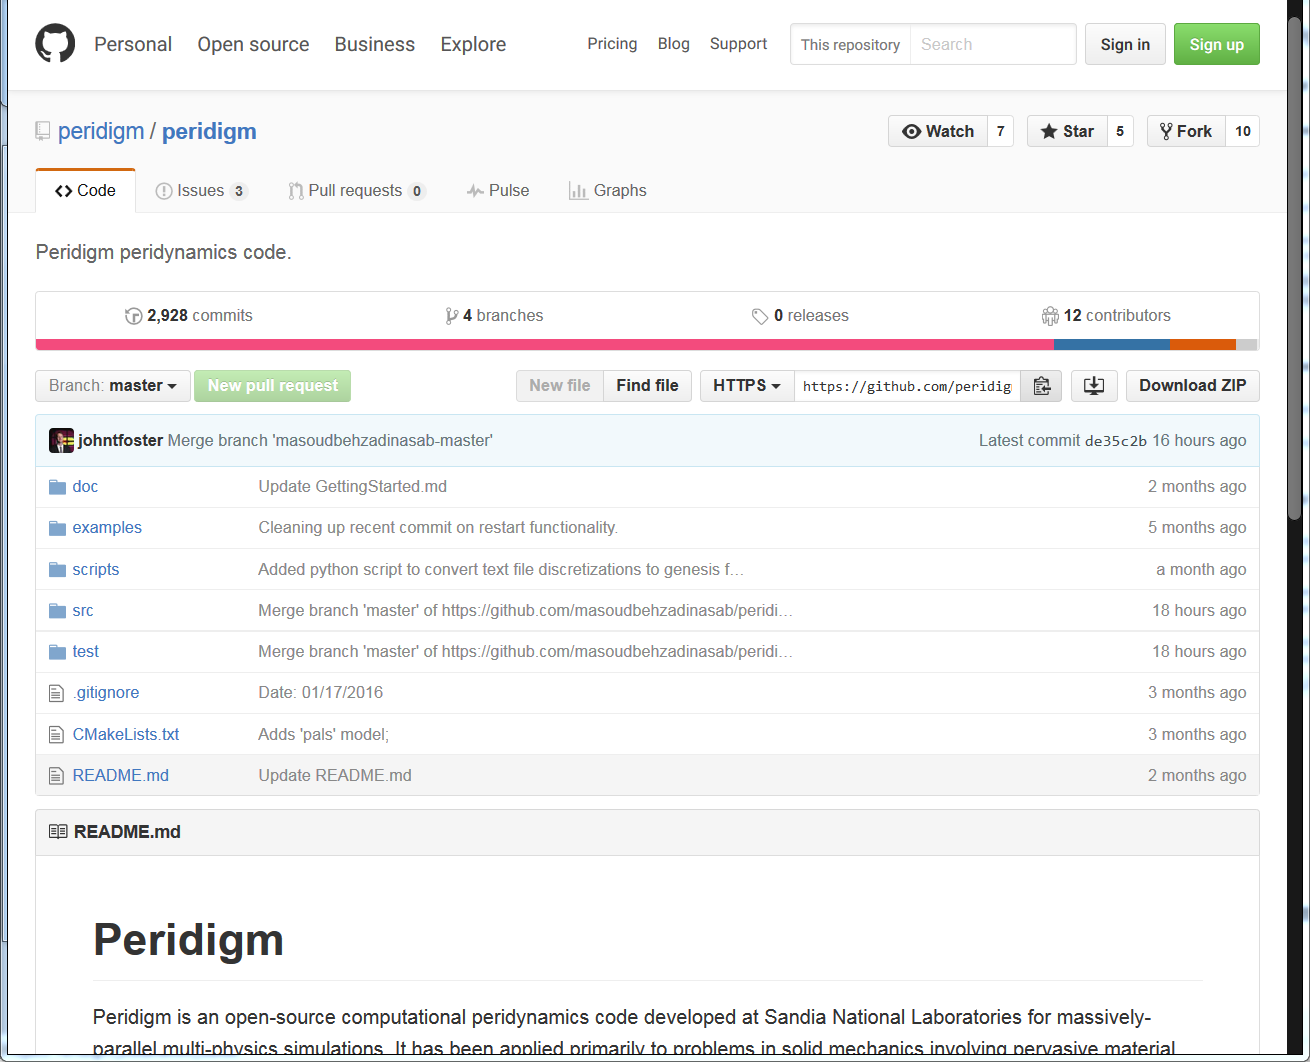
\includegraphics[width=0.95\linewidth]{Figures/Peridigm_GitHubRepository_Homepage_Master}};
   % Figure scope
   \begin{scope}[
     x={(image.south east)},
     y={(image.north west)},
   ]
     % Red rectangle Master
     \draw[red,ultra thick,rounded corners] (0.02,0.615) rectangle (0.1525,0.6575);
     % Red rectangle Download
     \draw[red,ultra thick,rounded corners] (0.8535,0.615) rectangle (0.9675,0.6575);
     % Help grid and labels
     %\pic{myimagegrid};
   \end{scope}
 \end{tikzpicture}
 \caption{\protect\marktool{\toolname} \protect\marktool{\githubname} repository screenshot}
 \label{fig:Peridigm_GitHubRepository_Homepage_Master}
\end{figure}

Unpack the archive:

\begingroup
\lstset{breaklines=true}
\begin{code}
cd $DOWNLOAD_DIR
unzip peridigm-master.zip
mv peridigm-master Peridigm-1.4.1-Source
\end{code}
\endgroup

\levelstay{Checkout the latest version from \texorpdfstring{\protect\marktool{\githubname{}}}{\githubname{}}}

\leveldown{With svn}

Use \marktool{kdesvn} to checkout the latest version. Checkout

\href{https://github.com/peridigm/peridigm.git/trunk}{https://github.com/peridigm/peridigm.git/trunk}

\levelstay{With git}

Use \marktool{git} on the cluster:

\begingroup
\lstset{breaklines=true}
\begin{code}
git clone https://github.com/peridigm/peridigm.git
\end{code}
\endgroup

\levelmultiup{Compiling \& installation}{2}

\marktool{\toolname} utilizes the \marktool{\cmakename} build system. It is recommended that Makefiles be created by running \verb+cmake+ from the command line, as opposed to using the \verb+ccmake+ GUI.

The installation here is described for the then official \marktool{\toolname} version 1.4.1. The steps for version 1.5 are identical besides the changes in folder names.

\marktool{\toolname} does not allow the use of the directory with the source-files for the further progress of the installation. Therefore, create a new folder

\begin{code}
mkdir Peridigm-1.4.1
\end{code}

and copy the file from section \ref{sec:Build-script_Peridigm} to the new folder. Change the lines for the library paths and the \marktool{\toolnameshort}-source-directory (last line) if necessary.

In order to use the script make it executable as described in section \ref{sec:Build-script_Executable}. Open a terminal as root, change directory to the created path and execute it with

\begin{code}
./cmake_peridigm.cmake > cmakeopts.log 2>&1
\end{code}

Once \marktool{\toolname} has been successfully configured, it can be compiled and installed as follows:

\begin{code}
make -j 4
make install
\end{code}

The default location for the created binary is \verb+/usr/local/bin/+. In case you want to create the binary at a different location add the following line to the script from section \ref{sec:Build-script_Peridigm}

\begin{code}
-D CMAKE_INSTALL_PREFIX=/PATH/TO/DESTINATION
\end{code}

After installation make sure to change permissions of the installation directory for the necessary users and groups.

\levelstay{After building and installing}

\cite{PeridigmUserGuide100} recommends to run \verb+ctest+ in your build directory after building and installing \marktool[\tooladdress]{\toolname} to run all tests and confirm that you have a clean build. Alternatively, \marktool[\tooladdress]{\toolname} offers an own test suite which is used here.

To be able to execute the test you first have to temporarily change the source and installation folder owner. Thus perform the following commands before executing the test.

\begin{code}
chown -R $USERNAME:$GROUPNAME Peridigm-1.4.1
chown -R $USERNAME:$GROUPNAME Peridigm-1.4.1-Source
\end{code}

Before starting the test-suite as a normal user, open a new shell or use an existing one and re-register your username to load the current state of the \verb+.bashrc+-file:

\begin{code}
su - $USERNAME
\end{code}

The \marktool[\tooladdress]{\toolname} test suite is then run from the terminal as non-root user as follows:

\begin{code}
make test
\end{code}

Remember to revert the modifications to the \marktool{\toolname} directory ownership after it is assured that all tests are passed with:

\begin{code}
chown -R root:root Peridigm-1.4.1
chown -R root:root Peridigm-1.4.1-Source
\end{code}

\levelstay{Install a local version on the cluster}

\begin{enumerate}[noitemsep]
  \item Login to the STM cluster and move to a directory of your convenience
  \item Clone your local \toolname{} version from GitHub with \verb+git clone+ or download the master zip-file and unpack, see section \ref{sec:Install:Peridigm:Download}
  \item Allocate cluster-node exclusively for building
\begin{code}
salloc --exclusive
\end{code}
  \item Load build and library environment
\begin{code}
. /cluster/software/slurm/etc/env.d/mpibuild.sh 
. /cluster/software/slurm/etc/env.d/peridigm.sh
\end{code}
  %\item Change directory to the local \toolname{} directory
\item Change directory to the folder, where the unpacked \toolname{} source folder is located
\begin{code}
cd ~/src/peridigm
\end{code}
  \item Create a build-directory and go to the new directory
\begin{code}
mkdir peridigm-build
cd peridigm-build
\end{code}
  \item Save the following lines in the file \texttt{cmake\_peridigm.cmake}. Change the path in the code to the correct location.
\begingroup
\lstset{breaklines=true}
\begin{code}
cmake \
-D CMAKE_BUILD_TYPE:STRING=Release \
-D CMAKE_INSTALL_PREFIX=/home/USER/peridigm-build \
-D CMAKE_CXX_FLAGS:STRING='-O2 -Wall -std=c++11 -pedantic -Wno-long-long -ftrapv -Wno-deprecated' \
/home/USER/peridigm-master
\end{code}
\endgroup
  \item Call \cmakename{} via terminal with the given code:
\begingroup
\lstset{breaklines=true}
\begin{code}
./cmake_peridigm.cmake
\end{code}
\endgroup
  \item Make
\begin{code}
make -j 8
\end{code}
  \item Test
\begin{code}
make test
\end{code}
  \item Create the executable 
\begin{code}
make install
\end{code}
  \item Exit salloc shell
\begin{code}
exit
\end{code}
  \item The executable is now located at \verb+~/src/peridigm/peridigm-build/bin+
  \item For how to execute the local version using the cluster queuing-system look at the \toolname{} User Guide
\end{enumerate}

A complete script for cloning \toolname{} from GitHub, compiling and installing on the cluster can be found in \autoref{sec:Build-script_Peridigm:Cluster}.

\levelstay{Use of \texorpdfstring{\protect\marktool{Docker}}{Docker}}

\href{http://johntfoster.github.io/posts/peridigm-without-building-via-Docker.html}{http://johntfoster.github.io/posts/peridigm-without-building-via-Docker.html} 

% \newpage
% \section{\protect\marktool{\paraviewname}}
% \setcounter{currentlevel}{5}
% %%%%%%%%%%%%%%%%%%%%%%%%%%%%%%%%%%%%
% Header                           %
%%%%%%%%%%%%%%%%%%%%%%%%%%%%%%%%%%%%
% 
% Revisions: 2017-04-10 Martin Rädel <martin.raedel@dlr.de>
%                       Initial draft
%               
% Contact:   Martin Rädel,  martin.raedel@dlr.de
%            DLR Composite Structures and Adaptive Systems
%          
%                                 __/|__
%                                /_/_/_/  
%            www.dlr.de/fa/en      |/ DLR
% 
%%%%%%%%%%%%%%%%%%%%%%%%%%%%%%%%%%%%
% Content                          %
%%%%%%%%%%%%%%%%%%%%%%%%%%%%%%%%%%%%

\marktool{\paraviewname} is an open source multiple-platform application for interactive, scientific visualization. The current release and further informations can be found on

\href{\paraviewaddress}{\paraviewaddress}

\marktool{\paraviewname} was developed to analyze extremely large datasets using distributed memory computing resources.

\leveldown{Linux installation}

\paragraph{Use 1-click install}

Go to

\href{https://software.opensuse.org/download/package?project=science\&package=paraview}{https://software.opensuse.org/download/package?project=science\&package=paraview}

and choose 1-Click-Install or download the rpm-file from the source.

\paragraph{Installation with \marktool{\opensusename}-repository} \marktool{\paraviewname} is part of the \marktool{\opensusename} Science Repository. The repository can be included into the package management.

\begingroup
\lstset{breaklines=true}
\begin{code}
zypper addrepo http://download.opensuse.org/repositories/science/openSUSE_Leap_42.1/science.repo
zypper refresh
zypper install paraview
\end{code}
\endgroup

\paragraph{Installation from source} The source code of the current \marktool{\paraviewname} release is available from the download section of the \marktool{\paraviewname} homepage. For an installation using the source code and \marktool{\cmakename} please consult

\href{http://www.paraview.org/Wiki/ParaView:Build\_And\_Install}{http://www.paraview.org/Wiki/ParaView:Build\_And\_Install}

\levelstay{Windows installation}

Go to the download section of the \marktool[\paraviewaddress]{\paraviewname} homepage and download the binary installers for your windows operating system architecture. Afterwards, simply run the executable installer and follow the instructions.

%%%%%%%%%%%%%%%%%%%%%%%%%%%%%%%%%%%%
% Package Usage                    %
%%%%%%%%%%%%%%%%%%%%%%%%%%%%%%%%%%%%

\chapter{Running \texorpdfstring{\protect\marktool{\toolnameshort}}{\toolnameshort{}}}
\setcounter{currentlevel}{6}
%%%%%%%%%%%%%%%%%%%%%%%%%%%%%%%%%%%%
% Header                           %
%%%%%%%%%%%%%%%%%%%%%%%%%%%%%%%%%%%%
% 
% Revisions: 2017-04-10 Martin Rädel <martin.raedel@dlr.de>
%                       Initial draft
%               
% Contact:   Martin Rädel,  martin.raedel@dlr.de
%            DLR Composite Structures and Adaptive Systems
%          
%                                 __/|__
%                                /_/_/_/  
%            www.dlr.de/fa/en      |/ DLR
% 
%%%%%%%%%%%%%%%%%%%%%%%%%%%%%%%%%%%%
% Content                          %
%%%%%%%%%%%%%%%%%%%%%%%%%%%%%%%%%%%%

A dedicated description on how to run \marktool{\toolname} can be found in the \marktool{\toolname} Users Guide which is part of the same repository as this document.

%%%%%%%%%%%%%%%%%%%%%%%%%%%%%%%%%%%%
% Package Usage                    %
%%%%%%%%%%%%%%%%%%%%%%%%%%%%%%%%%%%%

\chapter{Install \texorpdfstring{\protect\marktool{\paraviewname}}{\paraviewname{}}}
\setcounter{currentlevel}{6}
%%%%%%%%%%%%%%%%%%%%%%%%%%%%%%%%%%%%
% Header                           %
%%%%%%%%%%%%%%%%%%%%%%%%%%%%%%%%%%%%
% 
% Revisions: 2017-04-10 Martin Rädel <martin.raedel@dlr.de>
%                       Initial draft
%               
% Contact:   Martin Rädel,  martin.raedel@dlr.de
%            DLR Composite Structures and Adaptive Systems
%          
%                                 __/|__
%                                /_/_/_/  
%            www.dlr.de/fa/en      |/ DLR
% 
%%%%%%%%%%%%%%%%%%%%%%%%%%%%%%%%%%%%
% Content                          %
%%%%%%%%%%%%%%%%%%%%%%%%%%%%%%%%%%%%

\marktool{\paraviewname} is an open source multiple-platform application for interactive, scientific visualization. The current release and further informations can be found on

\href{\paraviewaddress}{\paraviewaddress}

\marktool{\paraviewname} was developed to analyze extremely large datasets using distributed memory computing resources.

\leveldown{Linux installation}

\paragraph{Use 1-click install}

Go to

\href{https://software.opensuse.org/download/package?project=science\&package=paraview}{https://software.opensuse.org/download/package?project=science\&package=paraview}

and choose 1-Click-Install or download the rpm-file from the source.

\paragraph{Installation with \marktool{\opensusename}-repository} \marktool{\paraviewname} is part of the \marktool{\opensusename} Science Repository. The repository can be included into the package management.

\begingroup
\lstset{breaklines=true}
\begin{code}
zypper addrepo http://download.opensuse.org/repositories/science/openSUSE_Leap_42.1/science.repo
zypper refresh
zypper install paraview
\end{code}
\endgroup

\paragraph{Installation from source} The source code of the current \marktool{\paraviewname} release is available from the download section of the \marktool{\paraviewname} homepage. For an installation using the source code and \marktool{\cmakename} please consult

\href{http://www.paraview.org/Wiki/ParaView:Build\_And\_Install}{http://www.paraview.org/Wiki/ParaView:Build\_And\_Install}

\levelstay{Windows installation}

Go to the download section of the \marktool[\paraviewaddress]{\paraviewname} homepage and download the binary installers for your windows operating system architecture. Afterwards, simply run the executable installer and follow the instructions.

%%%%%%%%%%%%%%%%%%%%%%%%%%%%%%%%%%%%
% Package Usage                    %
%%%%%%%%%%%%%%%%%%%%%%%%%%%%%%%%%%%%

\chapter{Install everything for \texorpdfstring{\protect\marktool{\fetranslatorname}}{\fetranslatorname{}}}
\setcounter{currentlevel}{6}
%%%%%%%%%%%%%%%%%%%%%%%%%%%%%%%%%%%%
% Header                           %
%%%%%%%%%%%%%%%%%%%%%%%%%%%%%%%%%%%%
% 
% Revisions: 2017-04-10 Martin Rädel <martin.raedel@dlr.de>
%                       Initial draft
%               
% Contact:   Martin Rädel,  martin.raedel@dlr.de
%            DLR Composite Structures and Adaptive Systems
%          
%                                 __/|__
%                                /_/_/_/  
%            www.dlr.de/fa/en      |/ DLR
% 
%%%%%%%%%%%%%%%%%%%%%%%%%%%%%%%%%%%%
% Content                          %
%%%%%%%%%%%%%%%%%%%%%%%%%%%%%%%%%%%%

\marktool{\fetranslatorname} is a \marktool{\javaname}-based tool to translate models between finite element software. \marktool{\fetranslatorname} implements the conversion of meshes from commercial FE tools into the format that \marktool{\toolname} is capable of using as a discretization for the creation of peridynamic collocation points.

In order to use the \marktool{\fetranslatorname} an implementation of the \marktool{\javaname} Runtime Environment (JRE) is necessary. To translate the mesh into binary format the tool \marktool{\ncgenname} from \marktool{\netcdfname} is required.

\leveldown{Linux}

\leveldown{Java}

\marktool{\opensusename} comes with a pre-installed version of the \marktool{openJDK} which is a free and open source implementation of the Java Platform, Standard Edition (Java SE). \marktool{openJDK} should be perfectly capable of running \marktool{\fetranslatorname}. To see if and which version of \marktool{\javaname} is installed on your system open a shell and type:

\begin{code}
java -version
\end{code}

However, since additions and changes to the \marktool{\fetranslatorname} can be necessary, a \marktool{\javaname}-capable IDE is required. The Oracle \marktool{\javaname} Development Kit (JDK) offers an integrated solution with the JRE and \marktool{\netbeansname} as IDE.

\leveldown{Install only \marktool{\javaname} development kit (JDK)}

\begin{enumerate}[noitemsep]
 \item Go to: \href{http://www.oracle.com/technetwork/java/javase/downloads/index.html}{http://www.oracle.com/technetwork/java/javase/downloads/index.html}
 \item Click on \textit{Java Platform (JDK)}
 \item Accept the License Agreement
 \item Open a shell and type \lstinline[style=inlinecodestyle]+lsb_release -a+ and check your operating system architecture (32bit: i586; 64bit: x86\_64)
 \item Click on the according \verb+rpm+ file for your Linux version (here: jdk-8u91-linux-i586.rpm for 32bit or jdk-8u91-linux-x64.rpm for 64bit, we use 64bit)
 \item In the dialog choose \textit{Save File} and save the file somewhere convenient on your system
 \item Open a root shell or a normal shell and switch to root user with
\begin{code}
su -
\end{code}
 \item Change directory to the folder where the RPM file is located
 \item Type
\begingroup
\lstset{breaklines = true}
\begin{code}
zypper install jdk-8u91-linux-x64.rpm
zypper install update-alternatives
update-alternatives --install /usr/bin/java java /usr/java/jdk1.8.0_91/bin/java 1065
update-alternatives --install /usr/bin/javac javac /usr/java/jdk1.8.0_91/bin/javac 1065
update-alternatives --install /usr/bin/jar jar /usr/java/jdk1.8.0_91/bin/jar 1065
update-alternatives --install /usr/bin/javaws javaws /usr/java/jdk1.8.0_91/bin/javaws 1065
update-alternatives --config java
java -version
nedit /home/$USERNAME/.bashrc &
\end{code}
\endgroup
 \item Add \lstinline[style=inlinecodestyle]+export JAVA_HOME=/usr/java/jdk1.8.0_91/+ to the \verb+.bashrc+-file
\end{enumerate}

\levelstay{Install \marktool{\javaname} development kit (JDK) with \marktool{\netbeansname}}

\begin{enumerate}[noitemsep]
 \item Go to: \href{http://www.oracle.com/technetwork/java/javase/downloads/index.html}{http://www.oracle.com/technetwork/java/javase/downloads/index.html}
 \item Click on \textit{NetBeans with JDK}
 \item Accept the License Agreement
 \item Open a shell and type \lstinline[style=inlinecodestyle]+lsb_release -a+ and check your operating system architecture (32bit: i586; 64bit: x86\_64)
 \item Click on the according \verb+sh+ file for your Linux version\\
 (here: \verb+jdk-8u91-nb-8_1-linux-x64.sh+)
 \item In the dialog choose \textit{Save File} and save the file somewhere convenient on your system
 \item Open a root shell or a normal shell and switch to root user with
\begin{code}
su -
\end{code}
 \item Change directory to the folder where the .sh file is located
 \item Change the installer file's permissions so it can be executed:
\begin{code}
chmod u+x <installer-file-name>
\end{code}
 \item Type
\begin{code}
./<installer-file-name>
\end{code}
 \item In the installation wizard:
 \begin{enumerate}
  \item At the Welcome page of the installation wizard, click \textit{Next}.
  \item At the JDK Installation page, specify the directory where to install the JDK, here \verb+/usr/local/java/jdk1.8.0_91+, and click \textit{Next}.
  \item At the \marktool{\netbeansname} IDE Installation page, do the following:
  \begin{itemize}
   \item Specify the directory for the \marktool{\netbeansname} IDE installation\\
   (here \verb+/usr/local/java/netbeans-8.1+)
   \item Accept the default JDK installation to use with the IDE or specify another JDK location.
  \end{itemize}
  \item Accept the default JDK installation to use with the IDE or specify another JDK location.
  \item Click \textit{Next}
  \item Review the Summary page to ensure the software installation locations are correct.
  \item Click \textit{Intall} to begin the installation.
  \item At the Setup Complete page, provide anonymous usage data if desired, and click \textit{Finish}
  \item When the installation is complete, you can view the log file, which resides in the following directory: \verb+~/.nbi/log.+
 \end{enumerate}
 \item Type
\begingroup
\lstset{breaklines = true}
\begin{code}
zypper install update-alternatives
update-alternatives --install /usr/bin/java java /usr/local/java/jdk1.8.0_91/bin/java 1065
update-alternatives --install /usr/bin/javac javac /usr/local/java/jdk1.8.0_91/bin/javac 1065
update-alternatives --install /usr/bin/jar jar /usr/local/java/jdk1.8.0_91/bin/jar 1065
update-alternatives --install /usr/bin/javaws javaws /usr/local/java/jdk1.8.0_91/bin/javaws 1065
update-alternatives --config java
java -version
nedit /home/$USERNAME/.bashrc &
\end{code}
\endgroup
 \item Add
\begin{code}
export JAVA_HOME=/usr/java/jdk1.8.0_91/
\end{code}
 and
\begin{code}
export PATH=$PATH:/usr/local/java/netbeans-8.1/bin
\end{code}
 to the \verb+.bashrc+-file
 \item Start a new shell with \verb+su - $USERNAME+ and type \verb+java -version+ to see if the correct version is active
 \item Start a new shell with \verb+su - $USERNAME+ and type \verb+netbeans &+ to start the IDE
 \item Perform update inside the IDE if asked for
\end{enumerate}

If problems occur during any \verb+update-alternatives --install+ try

% https://hschwarz77.wordpress.com/2015/08/14/install-java-alternatives/
\begingroup
\lstset{breaklines = true}
\begin{code}
update-alternatives --install /usr/bin/java java /usr/local/java/jdk1.8.0_91/bin/java 1
update-alternatives --install /usr/lib64/browser-plugins/javaplugin.so javaplugin /usr/local/java/jdk1.8.0_91/jre/lib/amd64/libnpjp2.so 1 --slave /usr/bin/javaws javaws /usr/local/java/jdk1.8.0_91/bin/javaws
update-alternatives --install /usr/bin/javac javac /usr/local/java/jdk1.8.0_91/bin/javac 1 --slave /usr/bin/jar jar /usr/local/java/jdk1.8.0_91/bin/jar
\end{code}
\endgroup

Now you can set the \marktool{\javaname} priorities with:

\begin{code}
update-alternatives --config java
update-alternatives --config javac
update-alternatives --config javaplugin
\end{code}

\levelup{\texorpdfstring{\protect\marktool{\netcdfname{}}}{\netcdfname{}}}

The \marktool{\netcdfname}-tool \marktool{\ncgenname} is required to convert the ascii mesh file into the binary format readable by \marktool{\toolname}. \marktool{\netcdfname} should already be installed to use \marktool{\toolname}. If the additions to the \verb+PATH+-variable from \autoref{sec:Install_netcdf} are set, no further actions have to be performed.

\levelup{Windows}

\leveldown{Java}

\begin{enumerate}[noitemsep]
 \item Go to: \href{http://www.oracle.com/technetwork/java/javase/downloads/index.html}{http://www.oracle.com/technetwork/java/javase/downloads/index.html}
 \item Click on \textit{NetBeans with JDK} for Development Kit and Netbeans or just \textit{Java Platform (JDK)}
 \item Perform the installation
\end{enumerate}

\levelstay{\texorpdfstring{\protect\marktool{\netcdfname{}}}{\netcdfname{}}}

To test the \marktool{\fetranslatorname} under Windows it is necessary to have \marktool{\ncgenname} available. \marktool{\ncgenname} is available as part of pre-built \marktool{\netcdfname} libraries. To install the latest release

\begin{enumerate}[noitemsep]
 \item Go to: \href{\netcdfaddress}{\netcdfaddress}
 \item Click \textit{Pre-built Windows Binaries for the latest version of \netcdfname}
 \item Go to \textit{Latest Release (\netcdfname{} X.Y.Z)}, here \netcdfname{} 4.4.0
 \item Download the executable matching your system, here netCDF4.4.0-NC4-64.exe
 \item Execute the installer
 \item Add the \verb+bin+ folder of the installation path, here \verb+D:\Programme\netCDF 4.4.0\+ to the Windows \verb+PATH+-Variable:
 \begin{enumerate}
  \item Open the \textit{Windows Control Panel} (Systemsteuerung)
  \item Open \textit{System}
  \item Click \textit{Advanced System Settings} (Erweiterte Systemeinstellungen)
  \item In the \textit{Advanced} tab open \textit{Environment Variables}
  \item Under \textit{User variables for USERNAME} select \verb+PATH+
  \item Click \textit{Edit}
  \item Under \textit{Value of the variable} add the path to the \verb+bin+ folder of the \marktool{\netcdfname} installation separated by a semicolon (\textit{;}), here: \verb+;D:\Programme\netCDF 4.4.0\bin\+
  \item Click \textit{OK} multiple times
 \end{enumerate}
\end{enumerate}

Now you can use \marktool{\ncgenname} in a command-window:

\begin{code}
ncgen.exe -o $OUTPUTFILENAME.g $INPUTFILENAME.g.ascii
\end{code}



%%%%%%%%%%%%%%%%%%%%%%%%%%%%%%%%%%%%
% Bibliography                     %
%%%%%%%%%%%%%%%%%%%%%%%%%%%%%%%%%%%%

\printbibliography

%%%%%%%%%%%%%%%%%%%%%%%%%%%%%%%%%%%%
% Appendix                         %
%%%%%%%%%%%%%%%%%%%%%%%%%%%%%%%%%%%%

%%%%%%%%%%%%%%%%%%%%%%%%%%%%%%%%%%%%
% Header                           %
%%%%%%%%%%%%%%%%%%%%%%%%%%%%%%%%%%%%
% 
% Revisions: 2017-04-10 Martin Rädel <martin.raedel@dlr.de>
%                       Initial draft
%               
% Contact:   Martin Rädel,  martin.raedel@dlr.de
%            DLR Composite Structures and Adaptive Systems
%          
%                                 __/|__
%                                /_/_/_/  
%            www.dlr.de/fa/en      |/ DLR
% 
%%%%%%%%%%%%%%%%%%%%%%%%%%%%%%%%%%%%
% Content                          %
%%%%%%%%%%%%%%%%%%%%%%%%%%%%%%%%%%%%

\begin{appendices}

\chapter{Build-scripts for Libraries}
\setcounter{currentlevel}{6}
%%%%%%%%%%%%%%%%%%%%%%%%%%%%%%%%%%%%
% Header                           %
%%%%%%%%%%%%%%%%%%%%%%%%%%%%%%%%%%%%
% 
% Revisions: 2017-04-10 Martin Rädel <martin.raedel@dlr.de>
%                       Initial draft
%               
% Contact:   Martin Rädel,  martin.raedel@dlr.de
%            DLR Composite Structures and Adaptive Systems
%          
%                                 __/|__
%                                /_/_/_/  
%            www.dlr.de/fa/en      |/ DLR
% 
%%%%%%%%%%%%%%%%%%%%%%%%%%%%%%%%%%%%
% Content                          %
%%%%%%%%%%%%%%%%%%%%%%%%%%%%%%%%%%%%

In the following sections, the build scripts for the libraries for \marktool{\toolname} are collected. These are Bash-scripts or \marktool{\cmakename}-files.

The scripts are taken from \href{https://peridigm.sandia.gov/}{https://peridigm.sandia.gov/} and modified slightly if necessary.

The files are provided with UTF-8 encoding. Please modify to your needs if necessary.

\leveldown{\texorpdfstring{\protect\marktool{\boostname{}}}{\boostname{}}}
\label{sec:Build-script_Boost}

\leveldown{\texorpdfstring{\protect\marktool{\boostname{}}}{\boostname{}} 1.55.0}

Open a text editor, copy the following code into a file and save as \verb+install_boost-1.55.0.sh+

\begingroup
\lstset{breaklines = true}
\lstinputlisting[
  style=scriptstyle,
  caption=Install script for \protect\marktool{\boostname} 1.55.0,
  label=lst:install_boost
]{Scripts/install_boost-1.55.0.sh}
\endgroup

\ifpdf
Alternatively, you can \textattachfile[author=raed_ma, color=0 0 1]{Scripts/install_boost-1.55.0.sh}{download} the script from within this document.
\fi

\levelstay{\texorpdfstring{\protect\marktool{\boostname{}}}{\boostname{}} 1.60.0}

Open a text editor, copy the following code into a file and save as \verb+install_boost-1.60.0.sh+

\begingroup
\lstset{breaklines = true}
\lstinputlisting[
  style=scriptstyle,
  caption=Install script for \protect\marktool{\boostname} 1.60.0,
  label=lst:install_boost-1.60.0
]{Scripts/install_boost-1.60.0.sh}
\endgroup

\ifpdf
Alternatively, you can \textattachfile[author=raed_ma, color=0 0 1]{Scripts/install_boost-1.60.0.sh}{download} the script from within this document.
\fi

\levelup{\texorpdfstring{\protect\marktool{\hdfname{}}}{\hdfname{}}}
\label{sec:Build-script_HDF}

Open a text editor, copy the following code into a file and save as \verb+install_hdf.sh+

\begingroup
\lstset{breaklines = true}
\lstinputlisting[
  style=scriptstyle,
  caption=Install script for \protect\marktool{\hdfname},
  label=lst:install_hdf
]{Scripts/install_hdf.sh}
\endgroup

\ifpdf
Alternatively, you can \textattachfile[author=raed_ma, color=0 0 1]{Scripts/install_hdf.sh}{download} the script from within this document.
\fi

\levelstay{\texorpdfstring{\protect\marktool{\netcdfname{}}}{\netcdfname{}}}
\label{sec:Build-script_NetCDF}

Open a text editor, copy the following code into a file and save as \verb+install_netcdf.sh+

\begingroup
\lstset{breaklines = true}
\lstinputlisting[
  style=scriptstyle,
  caption=Install script for \protect\marktool{\netcdfname},
  label=lst:install_netcdf
]{Scripts/install_netcdf.sh}
\endgroup

\ifpdf
Alternatively, you can \textattachfile[author=raed_ma, color=0 0 1]{Scripts/install_netcdf.sh}{download} the script from within this document.
\fi

% Other proposal from \href{http://diehlpk.github.io/2015/06/22/builing-peridigm.html}{http://diehlpk.github.io/2015/06/22/builing-peridigm.html}
% 
% \begin{code}
% # Set environment variables for MPI compilers
% export CC=mpicc
% export CXX=mpicxx
% export FC=mpif90
% export F77=mpif77
% 
% # 
% H5DIR=/usr/local/hdf5/ \
% export CPPFLAGS="-I${H5DIR}/include" \
% export LDFLAGS=-L${H5DIR}/lib \
% 
% # Configure NetCDF \
% CPPFLAGS="-I${H5DIR}/include" LDFLAGS=-L${H5DIR}/lib  ../configure --prefix=/usr/local/netcdf/  --disable-netcdf-4 --disable-dap --enable-parallel \
% 
% # Make, test, and install NetCDF
% make -j 8
% make check
% make install
% \end{code}

\levelstay{\texorpdfstring{\protect\marktool{\trilinosname{}}}{\trilinosname{}}}
\label{sec:Build-script_Trilinos}

Open an editor, copy the following code into the file and save as \verb+cmake_trilinos.cmake+. The final line marks the path to the \marktool{\trilinosname} source directory, which is named \verb+$DOWNLOAD_DIR+ in the documentation.

\begingroup
\lstset{breaklines = true}
\lstinputlisting[
  style=scriptstyle,
  caption=\protect\marktool{\cmakename} script for \protect\marktool{\trilinosname},
  label=lst:cmake_trilinos
]{Scripts/cmake_trilinos.cmake}
\endgroup

\ifpdf
Alternatively, you can \textattachfile[author=raed_ma, color=0 0 1]{Scripts/cmake_trilinos.cmake}{download} the script from within this document.
\fi

\levelstay{\texorpdfstring{\protect\marktool{\toolname{}}}{\toolname{}}}
\label{sec:Build-script_Peridigm}

\leveldown{\texorpdfstring{\protect\marktool{\cmakename{}}}{\cmakename{}} script for \texorpdfstring{\protect\marktool{\toolnameshort{}}}{\toolnameshort{}}}
\label{sec:Build-script_Peridigm:cmake}

Open an editor, copy the following code into the file and save as \verb+cmake_peridigm.cmake+. The final line marks the path to the \marktool{\toolname} source directory, which is named \verb+$DOWNLOAD_DIR+ in the documentation.

\begingroup
\lstset{breaklines = true}
\lstinputlisting[
  style=scriptstyle,
  caption=\protect\marktool{\cmakename} script for \protect\marktool{\toolnameshort},
  label=lst:cmake_peridigm
  ]{Scripts/cmake_peridigm.cmake}
\endgroup

\ifpdf
Alternatively, you can \textattachfile[author=raed_ma, color=0 0 1]{Scripts/cmake_peridigm.cmake}{download} the script from within this document.
\fi

\levelstay{Script for cloning \texorpdfstring{\protect\marktool{\toolnameshort{}}}{\toolnameshort{}} from GitHub and compiling on the STM-Cluster}
\label{sec:Build-script_Peridigm:Cluster}

\begingroup
\lstset{breaklines = true}
\lstinputlisting[
  style=scriptstyle,
  caption=Script for cloning \protect\marktool{\toolnameshort} from GitHub and compiling on the STM-Cluster,
  label=lst:shell_peridigm
  ]{Scripts/install_peridigm_github.sh}
\endgroup

\ifpdf
Alternatively, you can \textattachfile[author=raed_ma, color=0 0 1]{Scripts/install_peridigm_github.sh}{download} the script from within this document.
\fi

\levelup{Make a script executable}	\label{sec:Build-script_Executable}

In order to use a script file in the shell for installation you must first make the text file executable. Therefore, open a terminal, change directory to the folder the individual script is located and make the script executable for the user with

\begin{code}
chmod u+x $SCRIPTNAME.sh
\end{code}

\levelstay{Modifications of \texttt{.bashrc}}	\label{sec:Build-script_Bashrc}

When an interactive shell that is not a login shell is started, bash reads and executes commands from \verb+~/.bashrc+, if that file exists. You can find the \verb+.bashrc+ file in your user home directory \verb+/home/$USER/+ with \verb+ls -al+.

The following listings shows a modified \verb+.bashrc+ file which includes the exportation of the significant libraries in the \verb+$PATH+ and \verb+$LD_LIBRARY_PATH+ environment variables. The header is not printed.

\textbf{Be aware}:

\begin{itemize}[noitemsep]
 \item In case you use a 32bit operating system, or in some cases also for 64bit operating system, the lib64-folders must be changed to lib.
 \item The entries to the \verb+$PATH+ and \verb+$LD_LIBRARY_PATH+ variables should be added step-by-step \textbf{after} the installation of the individual tool. Otherwise, the install scripts might find pre-compiled items and use these instead of creating new binaries with the current settings.
\end{itemize}

\leveldown{\texttt{.bashrc} for \texorpdfstring{\protect\marktool{\toolnameshort{}}}{\toolnameshort{}} 1.4.1}

\begingroup
\lstset{breaklines = true}
\lstinputlisting[
  style=scriptstyle,
  firstline=28,
  caption=Modified .bashrc-file to set environment variables for \marktool{\toolname} 1.4.1,
  label=lst:bashrc_mod_1.4.1
]{Scripts/modified_bashrc.txt}
\endgroup

\ifpdf
You can \textattachfile[author=raed_ma, color=0 0 1]{Scripts/modified_bashrc.txt}{download} the file from within this document.
\fi

\levelstay{\texttt{.bashrc} for \texorpdfstring{\protect\marktool{\toolnameshort{}}}{\toolnameshort{}} 1.5}

\begingroup
\lstset{breaklines = true}
\lstinputlisting[
  style=scriptstyle,
  firstline=28,
  caption=Modified .bashrc-file to set environment variables for \marktool{\toolname} 1.5,
  label=lst:bashrc_mod_1.5
]{Scripts/modified_bashrc_Peridigm_1.5.txt}
\endgroup

\ifpdf
You can \textattachfile[author=raed_ma, color=0 0 1]{Scripts/modified_bashrc_Peridigm_1.5.txt}{download} the file from within this document.
\fi

\chapter{FAQ}
\setcounter{currentlevel}{6}
%%%%%%%%%%%%%%%%%%%%%%%%%%%%%%%%%%%%
% Header                           %
%%%%%%%%%%%%%%%%%%%%%%%%%%%%%%%%%%%%
% 
% Revisions: 2017-04-10 Martin R�del <martin.raedel@dlr.de>
%                       Initial draft
%               
% Contact:   Martin R�del,  martin.raedel@dlr.de
%            DLR Composite Structures and Adaptive Systems
%          
%                                 __/|__
%                                /_/_/_/  
%            www.dlr.de/fa/en      |/ DLR
%
%%%%%%%%%%%%%%%%%%%%%%%%%%%%%%%%%%%%
% Content                          %
%%%%%%%%%%%%%%%%%%%%%%%%%%%%%%%%%%%%

\chapter{FAQ}
\setcounter{currentlevel}{6}

\leveldown{\protect\toolname{}}

\begin{description}[leftmargin=\parindent,labelindent=\parindent,style=nextline]
% 
\item[When I call \marktool{\toolname} with \texttt{mpirun} I get an error that the program is unable to find the mesh file. What can I do? ]\mbox{}\\[-2.5\baselineskip]
  \begin{itemize}[noitemsep]
  \item This problem occurs for \marktool{\cubitname} mesh files (*.g)
  \item Before using them in a parallel job you have to decompose the mesh according to the number of processors to be used
  \item Please consult section \ref{sec:Peridigm:Run:Execution:Local:Input}
  \end{itemize}
%
\item[Everything works fine but when I call \marktool{decomp} I get a \texttt{***HDF5 library version mismatched error***} error. Why? ]\mbox{}\\[-2.5\baselineskip]
  \begin{itemize}[noitemsep]
  \item Check this same question in the \marktool{\toolname} Installation Guide from this same repository.
  \end{itemize}
%
\item[I get the following error message combination: \texttt{Throw test that evaluated to true: !boost::math::isfinite((*force)[i])} and \texttt{**** NaN returned by force evaluation.}. Why?]\mbox{}\\[-2.5\baselineskip]
  \begin{itemize}[noitemsep]
%   \item There seems to be no body load or non-zero kinematic boundary condition in your model.
%   \item See if the definition of \texttt{Body load} or \texttt{Prescribed Displacement} is working correctly in your model.
    \item It may be that your model became numerically unstable. Try to calculate the model again with a decreased value for the solver timestep safety factor.
  \end{itemize}
%
\item[I get the following error message: \texttt{**** Error:  getFieldId(), label not found:  Force} when using a \texttt{Compute Class Parameters}. Why?]\mbox{}\\[-2.5\baselineskip]
  \begin{itemize}[noitemsep]
    \item Make sure you request the \texttt{Variable} as a normal \texttt{Output Variable} as well. Have a look at the remarks in sections \ref{sec:Peridigm:QRG:ComputeClassParameters:Nodeset:Parameters}, \ref{sec:Peridigm:QRG:ComputeClassParameters:Block:Parameters} \& \ref{sec:Peridigm:QRG:ComputeClassParameters:NearestPoint:Parameters}.
    \item E.g. if your \texttt{Compute Class Parameter} is a force, \texttt{Force} must also be specified in the output section
  \end{itemize}
%
\item[I get the following error message: \texttt{Error!  An attempt was made to access parameter "ABC" of type "int" in the parameter (sub)list "ANONYMOUS"
using the incorrect type "double"!} in when using the function parser for an input parameter. Why?]\mbox{}\\[-2.5\baselineskip]
  \begin{itemize}[noitemsep]
    \item Make sure that the equation for the function parser does not result in a numerical value that can be expressed as an integer. E.g. With the values  \lstinline[style=inlinecodestyle]+#{DISPLACEMENT=1.0}+ and \lstinline[style=inlinecodestyle]+#{VELOCITY=1.0}+ the \texttt{Final Time} of a solver \lstinline[style=inlinecodestyle]+Final Time {DISPLACEMENT/VELOCITY}+ supposedly is 1.0. However, for the function parser the result is 1 as an integer. As a double value is expected for \texttt{Final Time} an error is thrown.
  \end{itemize}
%
\item[I get the following error message: \texttt{Error, the parameter "ABC" is not a list, it is of type "double"!} using the free format (.peridigm model). Why?]\mbox{}\\[-2.5\baselineskip]
  \begin{itemize}[noitemsep]
    \item Make sure there are no tabs in the line of ``ABS''. If there are, replace them with spaces and adjust the indentation of the line to the free format in your model.
  \end{itemize}
%
\item[Nothing happens when I use the \texttt{Implicit} solver and time-dependent \texttt{Prescribed Displacement}s. Why?]\mbox{}\\[-2.5\baselineskip]
  \begin{itemize}[noitemsep]
    \item This seems to be a bug in the calculation of the forces.
    \item See \href{https://github.com/peridigm/peridigm/issues/23}{https://github.com/peridigm/peridigm/issues/23}
  \end{itemize}
%
\end{description}

\levelstay{\protect\paraviewname{}}

% \levelstay{\protect\LaTeX}

%\input{\peridoccommonpath/Sections/Appendix_Linux_Commands}

\chapter{Non-necessary tools \& scripts}
\setcounter{currentlevel}{6}
%%%%%%%%%%%%%%%%%%%%%%%%%%%%%%%%%%%%
% Header                           %
%%%%%%%%%%%%%%%%%%%%%%%%%%%%%%%%%%%%
% 
% Revisions: 2017-04-10 Martin Rädel <martin.raedel@dlr.de>
%                       Initial draft
%               
% Contact:   Martin Rädel,  martin.raedel@dlr.de
%            DLR Composite Structures and Adaptive Systems
%          
%                                 __/|__
%                                /_/_/_/  
%            www.dlr.de/fa/en      |/ DLR
% 
%%%%%%%%%%%%%%%%%%%%%%%%%%%%%%%%%%%%
% Content                          %
%%%%%%%%%%%%%%%%%%%%%%%%%%%%%%%%%%%%

The installation is described for \marktool{\opensusename} for version 42.1.

\leveldown{\texorpdfstring{\protect\marktool{NEdit}}{NEdit}}

\marktool{NEdit}, the Nirvana editor, is a text editor and source code editor for the X Window System. For the installation of the editor \marktool{NEdit} visit:

\href{http://software.opensuse.org/download.html?project=editors\&package=nedit}{http://software.opensuse.org/download.html?project=editors\&package=nedit}

You can either choose the 1-Click-installation or add the repository and install manually. For the latter login to a terminal as \verb+root+ and type

\begingroup
\lstset{breaklines=true}
\begin{code}
zypper addrepo http://download.opensuse.org/repositories/editors/openSUSE_Leap_42.1/editors.repo
zypper refresh
zypper install nedit
\end{code}
\endgroup

% \levelstay{Script to clean tex directory}
% 
% \leveldown{Windows}
% 
% \begingroup
% \lstset{breaklines = true}
% \lstinputlisting[style=scriptstyle, language=command.com, extendedchars=true,]{clean_tex_directory.cmd}
% \endgroup

% \ifpdf
% Alternatively, you can \textattachfile[author=raed_ma, color=0 0 1]{clean_tex_directory.cmd}{download} the script from within this document.
% \fi

\levelstay{RM-\LaTeX}	\label{sec:RM_LaTeX}

Download the package via the intranet (from within the DLR network or via a VPN connection):

\href{teamsites.dlr.de/rm/latex/SitePages/Homepage.aspx}{teamsites.dlr.de/rm/latex/SitePages/Homepage.aspx}

Follow the instructions given in \verb+/doc/RM-LaTeX-Guide/RM-LaTeX-Guide.pdf+.

\leveldown{Linux}

Before using \verb+mktexlsr+ set

\begin{code}
chmod +t texmf/
\end{code}

and

\begin{code}
chmod go+w texmf/
\end{code}

Due to some problems in the RM-\LaTeX{} package meaningful use is only possible under Windows. If using with Linux do not use everything related to the package \verb+dlrsecondpage+.

\levelstay{Windows}

There should be no additional steps necessary.

\chapter{This document}
\setcounter{currentlevel}{6}

%%%%%%%%%%%%%%%%%%%%%%%%%%%%%%%%%%%%
% Header                           %
%%%%%%%%%%%%%%%%%%%%%%%%%%%%%%%%%%%%
% 
% Revisions: 2017-04-10 Martin Rädel <martin.raedel@dlr.de>
%                       Initial draft
%               
% Contact:   Martin Rädel,  martin.raedel@dlr.de
%            DLR Composite Structures and Adaptive Systems
%          
%                                 __/|__
%                                /_/_/_/  
%            www.dlr.de/fa/en      |/ DLR
% 
%%%%%%%%%%%%%%%%%%%%%%%%%%%%%%%%%%%%
% Content                          %
%%%%%%%%%%%%%%%%%%%%%%%%%%%%%%%%%%%%

\chapter{This document}
\setcounter{currentlevel}{6}

\leveldown{Repository}

%%%%%%%%%%%%%%%%%%%%%%%%%%%%%%%%%%%%
% Header                           %
%%%%%%%%%%%%%%%%%%%%%%%%%%%%%%%%%%%%
% 
% Revisions: 2017-04-10 Martin R�del <martin.raedel@dlr.de>
%                       Initial draft
%               
% Contact:   Martin R�del,  martin.raedel@dlr.de
%            DLR Composite Structures and Adaptive Systems
%          
%                                 __/|__
%                                /_/_/_/  
%            www.dlr.de/fa/en      |/ DLR
% 
%%%%%%%%%%%%%%%%%%%%%%%%%%%%%%%%%%%%
% Content                          %
%%%%%%%%%%%%%%%%%%%%%%%%%%%%%%%%%%%%

This document is part of the \reponame{} repository. The complete repository can be found at:

\href{\repoaddress}{\repoaddress}

\levelstay{Typesetting}

%%%%%%%%%%%%%%%%%%%%%%%%%%%%%%%%%%%%
% Header                           %
%%%%%%%%%%%%%%%%%%%%%%%%%%%%%%%%%%%%
% 
% Revisions: 2017-04-10 Martin R�del <martin.raedel@dlr.de>
%                       Initial draft
%               
% Contact:   Martin R�del,  martin.raedel@dlr.de
%            DLR Composite Structures and Adaptive Systems
%          
%                                 __/|__
%                                /_/_/_/  
%            www.dlr.de/fa/en      |/ DLR
% 
%%%%%%%%%%%%%%%%%%%%%%%%%%%%%%%%%%%%
% Content                          %
%%%%%%%%%%%%%%%%%%%%%%%%%%%%%%%%%%%%


This document was originally typeset using the documentclass \texttt{dlrreprt} from the DLR-internal RM-\LaTeX{} package.

The RM-\LaTeX{} package is not publicly available. Therefore, this document is compatible with a bootstrap-version of the documentclass, called \texttt{bootstrap\_dlrreprt}. \texttt{bootstrap\_dlrreprt} class is part of this repository.

The compilation is performed with \verb+pdflatex+ with the following options:

\begingroup
\lstset{breaklines=true}
\begin{texcode}
pdflatex --shell-escape -synctex=1 -interaction=nonstopmode %source --extra-mem-top=60000000
\end{texcode}
\endgroup

The bibliography is compiled with \verb+biber+. The glossary must be compiled with makeindex or, for \windowsosname{}, the included batch-script may be used. The keyword index is created automatically.

The general compilation order is:

\verb+pdflatex+ $\rightarrow$
\verb+biber+ $\rightarrow$
\verb+makeindex+ $\rightarrow$
\verb+pdflatex+ $\rightarrow$
\verb+pdflatex+


\end{appendices}

% \chapter*{\rlap{BSD Documentation License}}
\chapter*{BSD Documentation License}
\phantomsection  % so hyperref creates bookmarks
\addcontentsline{toc}{chapter}{BSD Documentation License}
\label{sec:Appendix:License}

% \begin{verbatim}
\begingroup
\lstset{%
  breaklines=true,%
  breakindent=\parindent,
  xleftmargin=\parindent,%
  xrightmargin=\parindent,%
}
\begin{code}
Redistribution and use in source (Docbook format) and 'compiled' forms (PDF, PostScript, HTML, RTF, etc), with or without modification, are permitted provided that the following conditions are met:

1. Redistributions of source code (Docbook format) must retain the above copyright notice, this list of conditions and the following disclaimer.

2. Redistributions in compiled form (transformed to other DTDs, converted to PDF, PostScript, HTML, RTF, and other formats) must reproduce the above copyright notice, this list of conditions and the following disclaimer in the documentation and/or other materials provided with the distribution.

3. The name of the author may not be used to endorse or promote products derived from this documentation without specific prior written permission.

THIS DOCUMENTATION IS PROVIDED BY THE AUTHOR ``AS IS AND ANY EXPRESS OR IMPLIED WARRANTIES, INCLUDING, BUT NOT LIMITED TO, THE IMPLIED WARRANTIES OF MERCHANTABILITY AND FITNESS FOR A PARTICULAR PURPOSE ARE DISCLAIMED. IN NO EVENT SHALL THE AUTHOR BE LIABLE FOR ANY DIRECT, INDIRECT, INCIDENTAL, SPECIAL, EXEMPLARY, OR CONSEQUENTIAL DAMAGES (INCLUDING, BUT NOT LIMITED TO, PROCUREMENT OF SUBSTITUTE GOODS OR SERVICES; LOSS OF USE, DATA, OR PROFITS; OR BUSINESS INTERRUPTION) HOWEVER CAUSED AND ON ANY THEORY OF LIABILITY, WHETHER IN CONTRACT, STRICT LIABILITY, OR TORT (INCLUDING NEGLIGENCE OR OTHERWISE) ARISING IN ANY WAY OUT OF THE USE OF THIS DOCUMENTATION, EVEN IF ADVISED OF THE POSSIBILITY OF SUCH DAMAGE.
\end{code}
\endgroup
% \end{verbatim}

\end{document}
